\documentclass{willowtreebook}
\usepackage{url}
\usepackage{tikz}
\usepackage{quiver}
\usetikzlibrary{shapes}
\usetikzlibrary{decorations.pathreplacing}
\usetikzlibrary{hobby,backgrounds,calc,trees}
\colorlet{lgray}{gray!25}
\colorlet{llgray}{gray!50}
\usepackage{tikz-cd}
\usepackage{sseq}


\newcommand{\nc}{\newcommand}
\nc{\ul}{\underline}
\nc{\dmo}{\DeclareMathOperator}
\dmo{\Rep}{Rep}
\dmo{\Sub}{Sub}
\dmo{\Vect}{Vect}
\dmo{\co}{co}
\dmo{\hocolim}{hocolim}
\dmo{\colim}{colim}
\dmo{\Ch}{Ch}
\dmo{\fib}{fib}
\dmo{\cofib}{cofib}
\nc{\bbZ}{\mathbb{Z}}
\nc{\bbR}{\mathbb{R}}
\nc{\bbF}{\mathbb{F}}
\nc{\bbC}{\mathbb{C}}
\dmo{\Sets}{Set}
\nc{\cat}[1]{\mathscr{#1}}
\nc{\Mid}{\,\big|\,}
\nc{\normal}{\trianglelefteq}
\nc{\SET}[2]{\big\{\,#1\Mid#2\,\big\}}
\dmo{\coeff}{coeff}
\dmo{\Mack}{Mack}
\dmo{\Ho}{Ho}
\dmo{\LFun}{LFun}
\dmo{\Fun}{Fun}
\dmo{\Alg}{Alg}
\dmo{\FinSet}{Fin}
\dmo{\End}{End}
\dmo{\Ext}{Ext}
\dmo{\sSet}{sSet}
\dmo{\Stab}{Stab}
\dmo{\Kan}{Kan}
\dmo{\Quillen}{Quillen}
\dmo{\Top}{Top}
\dmo{\Inf}{Inf}
\dmo{\ev}{ev}
\dmo{\Conj}{Conj}
\dmo{\Mod}{Mod}
\dmo{\Res}{Res}
\dmo{\Ind}{Ind}
\dmo{\Coind}{Coind}
\dmo{\Grp}{Grp}
\dmo{\Sp}{Sp}
\dmo{\SSp}{SeqSp}
\dmo{\Aut}{Aut}
\dmo{\Iso}{Iso}
\dmo{\Map}{Map}
\dmo{\sgn}{sgn}
\dmo{\Ab}{Ab}
\dmo{\Hom}{Hom}
\dmo{\id}{id}
\usepackage{physics}
\pgfdeclarelayer{background}
\pgfsetlayers{background,main}
%%Alternative command for C_p-Lewis diagrams
\newcommand{\lew}[5]{
\begin{tikzcd}
    #1 \arrow[d, "#3", curve={height=3pt}, swap, shift right=2] \\
    #2 \arrow[u, "#4", swap, curve={height=3pt}, shift right=2] \arrow[loop, "#5", distance=20, out=300,in=240]
\end{tikzcd}
}

\Title{MA8403  - Equivariant homotopy theory}
\Author{Drew Heard}
\BibliographyFile{ma8403} 		
	% The name of the .bib file, without file extension.
\begin{document}
\chapter{Preface}
This are the courses notes for MA8403 - Equivariant homotopy theory, held during the Autumn semester 2023 at NTNU. The notes are mainly based on two excellent sets of lectures notes, one by Guillou \cite{guillou}, and one by Blumberg \cite{blumberg}. The notes will be continually updated during the semester. 
\afterpreface
\chapter{Equivariance in algebra}
\subsection{Group actions in algebra}
We recall that if $X$ is an object in a category $\cat C$, then the set of endomorphisms $\End(X)$ forms a monoid (that is, a set equipped with an associative binary operation and an identity element) under composition. The set of automorphisms of $X$ (that is, those endomorphisms that are invertible) form a group. Moreover, we have
\[
\Aut(X) = \End(X) \cap \Iso(\cat C)
\]

Note that any group is a monoid, simply by forgetting the existence of inverses. 
\begin{definition}\label{def:group-action}
    An action of a group $G$ on an object $X \in \cat C$ is a monoid homomorphism $a \colon G \to \End(X)$, or equivalently a group homomorphism $a \colon G \to \Aut(X)$ (note that a monoid homomorphism between groups is a group homomorphism). 
\end{definition}
\begin{remark}
    Unwinding the definition, this means that we have:
    \begin{enumerate}
        \item For each $g \in G$, there is a morphism $a(g) \colon X \to X$.
        \item $a$ preserves composition, i.e., $a(g \cdot h) = a(g) \cdot a(h)$. 
        \item $a$ preserves identifies, so $a(e) = \id_X$.
    \end{enumerate}
\end{remark}
\begin{example}
    Let $\cat C$ be the category of sets and functions. Then, $a \colon G \to \End(X) = \big\{\,f \colon X \to X\big\}$ correspond to a function $\overline{a} \colon G \times X \to X$. The conditions above mean that the diagrams
    % https://q.uiver.app/#q=WzAsNCxbMCwwLCJHIFxcdGltZXMgRyBcXHRpbWVzIFgiXSxbMCwxLCJHIFxcdGltZXMgWCJdLFsxLDAsIkcgXFx0aW1lcyBYIl0sWzEsMSwiWCJdLFswLDEsIlxcaWQgXFx0aW1lcyBcXG92ZXJsaW5le2F9IiwyXSxbMCwyLCJtIFxcdGltZXMgXFxpZCJdLFsyLDMsIlxcb3ZlcmxpbmV7YX0iXSxbMSwzLCJcXG92ZXJsaW5le2F9IiwyXV0=
\[\begin{tikzcd}[ampersand replacement=\&]
	{G \times G \times X} \& {G \times X} \\
	{G \times X} \& X
	\arrow["{\id \times \overline{a}}"', from=1-1, to=2-1]
	\arrow["{m \times \id}", from=1-1, to=1-2]
	\arrow["{\overline{a}}", from=1-2, to=2-2]
	\arrow["{\overline{a}}"', from=2-1, to=2-2]
\end{tikzcd}
\text{ and }
% https://q.uiver.app/#q=WzAsNCxbMCwwLCJcXHtcXGFzdFxcfSBcXHRpbWVzIFgiXSxbMSwwLCJHIFxcdGltZXMgWCJdLFswLDEsIlgiXSxbMSwxLCJYIl0sWzAsMSwiZSBcXHRpbWVzIFxcaWQiXSxbMCwyLCJcXGNvbmciLDJdLFsxLDMsIlxcb3ZlcmxpbmV7YX0iXSxbMiwzLCIiLDIseyJsZXZlbCI6Miwic3R5bGUiOnsiaGVhZCI6eyJuYW1lIjoibm9uZSJ9fX1dXQ==
\begin{tikzcd}[ampersand replacement=\&]
	{\{\ast\} \times X} \& {G \times X} \\
	X \& X
	\arrow["{e \times \id}", from=1-1, to=1-2]
	\arrow["\cong"', from=1-1, to=2-1]
	\arrow["{\overline{a}}", from=1-2, to=2-2]
	\arrow[Rightarrow, no head, from=2-1, to=2-2]
\end{tikzcd}\]
commute, where $m \colon G \times G \to G$ denotes the group multiplication. Equivalently, in symbols, we have
\[
\overline{a}(g,\overline{a}(h,x)) = \overline{a}(gh,x) 
\]
and
\[
\overline{a}(e,x) = x. 
\]
\end{example}
\begin{remark}
    Let $BG$ denote the category with one object $\ast$ and with $\Hom(\ast,\ast) = G$. Then an action of $G$ in the category $\cat C$ is the same as a functor $\rho \colon BG \to \cat C$. The object $X$ in the previous definition is the object $\rho(\ast) \in \cat C$. 
\end{remark}
\begin{remark}
    Let $\cat C = \Mod_R$ for a commutative ring $R$. An action of $G$ on $M \in \Mod_R$ is a monoid homomorphism
    \[
a \colon G \to \Hom_R(M,M).
    \]
    We recall that $\Hom_R(M,M)$ actually has the structure of an $R$-algebra
\end{remark}
\begin{definition}
    The ($R$-linear) group ring on $R$ is the $R$-algebra $R[G]$ whose:
    \begin{enumerate}[label=(\alph*)]
    \item underlying $R$-module is the free $R$-module with basis on the underlying set of $G$. 
    \item whose multiplication is given on basis elements by the group operation. 
    \end{enumerate}
\end{definition}
\begin{example}
    Let $R = \mathbb{Z}$ and $G = C_2 = \langle \sigma \rangle$. An element of $\bbZ[C_2]$ is of the form $a + b\sigma$ where $a,b \in \bbZ$. Multiplication is given by
    \[
(a_1 \cdot 1+b_1\sigma)\cdot(a_2\cdot 1+b_2\sigma) = (a_1a_2+b_1b_2)\cdot 1  + (a_1b_2+b_1a_2)\sigma. 
    \]
    This is the same thing as the polynomial ring $\bbZ[\sigma]/(\sigma^2-1)$. 
\end{example}
\begin{remark}
    Categorically, the group ring construction is left adjoint to the functor that takes an $R$-algebra to its group of units, i.e., there is an adjudication
    \[
R[-] \colon \Grp \leftrightarrows \Alg_R \colon (-)^{
\times}
    \]
\end{remark}
Returning to group actions, we have the following:
\begin{proposition}
    Let $R$ be a commutative ring, and $G$ a finite group. The following data on an $R$-module $M$ are equivalent:
    \begin{enumerate}
        \item A monoid homomorphism $G \to \End_R(M)$.
        \item A group homomorphism $G \to \Aut_R(M)$. 
        \item A homomorphism of $R$-algebras $R[G] \to \Hom_R(M,M)$. 
        \item An $R[G]$-module structure on $M$ whose underlying $R$-module structure is $M$. 
    \end{enumerate}
\end{proposition}
\begin{definition}
    A representation of $G$ over $R$ is an $R[G]$-module. 
\end{definition}
\begin{example}
    If $R = k$ is a field, then the underlying $R$-module is a $k$-vector space $V$. If $\dim_k(V) = n$, then $\Aut_k(V) = GL_n(k)$, and a $k$-representation is the same thing as a group homomorphism $G \to GL_n(k)$. 
\end{example}
\begin{definition}
    The $R[G]$-module $R[G]$ is known as the regular representation. More generally, if $X$ is a finite $G$-set, then the free $R$-module $R[X]$ inherits the structure of a $R[G]$-module (the case of $R[G]$ itself corresponds to the finite $G$-set $G$, considered as an $R[G]$-module over itself). Representations obtained this way are known as permutation representations. 
\end{definition}
\begin{example}
    Taking $X$ to be the trivial $G$-set, we obtain the (one-dimensional) trivial representation. This is simply the $R[G]$-module $R$, where $G$ acts trivially. 
\end{example}
\begin{definition}
    Let $G = C_2 = \langle \tau \rangle$, and suppose that $-1 \ne 1 \in R$. Then the sign representation of $G$ is the one-dimensional representation where $\tau$ acts as $-1$ (if $-1 = 1$ in $R$ this still makes sense, but is just the trivial representation). Note that this is an example of a representation that is not a permutation representation.
\end{definition}
\begin{example}
    Let $C_n = \langle \sigma \rangle$ be the cyclic group of order $n$. Let us calculate all complex 1-dimensional representations of $C_n$, i.e., homomorphisms $\rho \colon C_n \to \mathbb{C}$. Note that if we define $\rho(\sigma) =c$, then $\rho(\sigma^n) = c^n = 1$, so that $c$ must be an $n$-th root of unity. There are precisely $n$-of these (take $\zeta_n = e^{2\pi/n i}$), and so there are precisely $n$-representations. For example, when $G = C_4$, the four representations correspond to sending $\sigma$ to either $1,i,-1$ or $-i$. Note that we can also consider these as 2-dimensional \emph{real} representations. 
\end{example}
\begin{notation}
We let $\rho = \rho_G$ denote the regular representation of $G$, and the trivial $n$-dimensional representation by $\mathbf{n} = R^{\oplus n}$. 
\end{notation}
\begin{definition}
    A subrepresentation is a submodule. 
\end{definition}
\begin{example}
    The regular representation always has a one-dimensional trivial representation, generated by the sum $\sum_{g \in G}g$. 
\end{example}
\begin{definition}
    A representation $V$ is irreducible if the only subrepresentations of $V$ are $0$ and $V$. 
\end{definition}
\begin{theorem}[Maschke]Suppose that $k$ is a field of characteristic not dividing $|G|$. Then every
representation splits as a direct sum of irreducible representations.
\end{theorem}
\begin{proof}
    We prove the following: if $V \subseteq W$ is a subrepresentation, then there exists $U \subseteq W$ such that $U \oplus V \simeq W$. 

    To see this, let $\pi \colon W \to W$ be any $k$-linear projection of $W$ onto $V$. This map need not be $G$-equivariant, but we can make it so by `averaging'. That is, we define a new map $\phi \colon W \to W$ by 
    \[
\phi(\mathbf{w}) = \frac{1}{|G|}\sum_{g \in G}g \cdot \pi(g^{-1} \cdot \mathbf{w}). 
    \]
   Moreover the map is $G$-equivariant: for $h \in G$ we have
   \[
   \begin{split}
\phi(h \cdot \mathbf{w}) &= \frac{1}{|G|}\sum_{g \in G}g \cdot \pi(g^{-1} \cdot h \cdot \mathbf{w}) \\
& = \frac{1}{|G|}\sum_{u \in G}u \cdot h \cdot \pi(u^{-1} \cdot \mathbf{w}) \\
&= h \cdot \phi(\mathbf{w}),
\end{split}
   \]
   where $u = gh^{-1}$, and so $\phi$ is $k[G]$-linear. Furthermore, the map $\phi$ is the identity on $V$ By the splitting lemma, $W = V \oplus \ker(\phi)$. 
\end{proof}
\begin{remark}
We used the assumption on $k$ to ensure that we could divide by $|G|$. Without that assumption, the theorem is false. Indeed, let $G = C_2$, $R = \mathbb{F}_2$ and consider the representation defined by $\rho(\tau) =\begin{pmatrix}
1 & 1 \\
1 & 0 
\end{pmatrix} $. This is not irreducible, but does not split as a direct sum of irreducible representations. 
\end{remark}
\begin{corollary}
Suppose that $k$ is a field of characteristic not dividing $|G|$.  If $V$ is an irreducible representation, then $V$ is isomorphism to a submodule of $k[G]$ (slogan: all irreducibles are submodules of the regular representation). 
\end{corollary}
\begin{proof}
    Let $\mathbf{v} \in V$ be non-trivial. Then the homomorphism $\phi \colon k[G] \to V$ given by sending $1$ to $\mathbf{v}$ must be surjective, because $V$ is irreducible. Let $U = \ker(\phi)$, then apply Maschke's theorem. 
\end{proof}
\begin{example}
    Let $G = C_2 = \langle \tau \rangle$, and $k$ a field of characteristic not equal to 2. We have the trivial representation $\mathbf{1}$ and the sign representation $\mathbf{1}_{\sgn}$. Then, $\mathbf{1}$ is generated by the sum $1+\tau$, while $\mathbf{1}_{\sgn}$ is generated by $1-\tau$, and we deduce that 
    \[
\rho_{C_2} = \mathbf{1} \oplus \mathbf{1}_{\sgn}. 
    \]
\end{example}
\section{The representation ring}
Let $k$ be a field, and suppose that $V$ and $W$ are $G$-representations, then the $k$-linear tensor sum $V \oplus W$ can be given the structure of a $k[G]$-module, by taking the diagonal $G$-action. If we think of a representation in terms of a homomorphism $\rho \colon G \to GL_n(k)$, then this direct sum corresponds to the `block sum'
\[
G \to GL_n(k) \times GL_m(k) \to GL_{n+m}(k)
\]
Similarly, we can define a tensor product of representations using the `Kronecker tensor product' (or matrix direct product). Equivalently, this is the $k$-linear tensor product $V \otimes W$ with the $g$-action defined on simple tensors by
\[
g \cdot (\mathbf{v} \otimes\mathbf{w}) = g \cdot \mathbf{v} \otimes g \mathbf{w}. 
\]
We leave it for the reader to verify the following straightforward computations:
\begin{enumerate}[label=(\alph*)]
    \item $\mathbf{1} \otimes V \cong V \cong V \otimes \mathbf{1}$. 
    \item $\mathbf{n} \otimes V \cong V^{\oplus n} \cong V \otimes \mathbf{n}$. 
\end{enumerate}
\begin{example}[label=ex:tensor-product-sign]
    Let us compute the tensor product $\mathbf{1}_{\sgn} \otimes \mathbf{1}_{\sgn}$. The underlying vector space is simply $k \otimes k \cong k$, while $\tau$ acts as $\tau \cdot (1 \otimes 1) = (\tau \cdot 1) \otimes (\tau \cdot 1) = -1 \otimes -1 = 1 \otimes 1$. So the tensor product $\mathbf{1}_{\sgn} \otimes \mathbf{1}_{\sgn} = \mathbf{1}$. 
   
\end{example}
\begin{example}[label=ex:tensor-product-c3]
    Take $G = C_3$ and $k = \mathbb{R}$. We have a two-dimensional representation $\lambda_3$ corresponding to rotation by an angle of $2\pi/3$. What is $\lambda_3 \otimes \lambda_3$? This is a 4-dimensional representation, and by working out all irreducible representations must be either $\mathbf{4}, \mathbf{2} \oplus \lambda_3$ or $\lambda_3 \oplus \lambda_3$. If you know a little bit of character theory, you can see that it must be $\mathbf{2} \oplus \lambda_3$: we have
    \[
\chi_{\lambda_3 \otimes \lambda_3}(1) = 4, \quad \chi_{\lambda_3 \otimes \lambda_3}(\tau) = 1
    \]
        \[
\chi_{\mathbf{4}}(1) = 4, \quad \chi_{\mathbf{4}}(\tau) =     4
    \]
        \[
\chi_{\mathbf{2} \oplus \lambda_3}(1) = 4, \quad \chi_{\mathbf{2} \oplus \lambda_3}(\tau) = 1
    \]
            \[
\chi_{\lambda_3 \oplus \lambda_3}(1) = 4, \quad \chi_{\lambda_3  \oplus \lambda_3}(\tau) = -2
    \]
\end{example}
\begin{remark}
    By passing to isomorphism classes of representations, the set of finite dimensional representations has the structure of a semiring. Using the Grothendieck construction, we can produce a commutative ring. 
\end{remark}
\begin{definition}
    For a finite group $G$ the real representation ring $RO(G)$ is the Grothendieck group of the above semi-ring. Explicitly,
    \[
RO(G) \coloneqq \mathbb{Z}\left\{ \parbox{15em}{isomorphism classes of finite-dimensional real $G$-representations} \right\}/\langle [ V \oplus W] - [V] - [W] \rangle .
    \]
\end{definition}
\begin{remark}
    As an abelian group, $RO(G)$ is a direct sum of copies of $\bbZ$, with rank equal to the number of isomorphism classes of irreducible representations. 
\end{remark}
\begin{remark}
    We can make the same definition for other fields, for example when $k = \mathbb{C}$ we get the complex representation ring $R(G)$. 
\end{remark}
\begin{example}
    We have $RO(C_2) \cong \bbZ\{ \mathbf{1} \} \oplus \bbZ\{\mathbf{1}_{\sgn}\}$. The ring structure is determined by Example~\eqref{ex:tensor-product-sign}: we have $RO(C_2) \cong \bbZ[\sigma]/(\sigma^2-1)$. The same is true for the complex representation ring. Note that this is the same as $\bbZ[C_2]$. In fact, the complex representation ring of a finite abelian group is always (non-canonically) isomorphic to the group ring: it is the group ring of the character group. 
\end{example}
\begin{example}
    When $G = C_3$ we have that
    \[
RO(C_3) = \bbZ\{ \mathbf{1} \} \oplus \bbZ\{ \lambda_3 \}. 
    \]
    By Example~\eqref{ex:tensor-product-c3} we have $[\lambda_3]^2 = 2 + [\lambda_3]$ and we see that
    \[
RO(C_3) \cong \bbZ[\lambda]/(\lambda^2-\lambda-2). 
    \]
    On the other hand, the complex representation ring is given by \[
    R(C_3) \cong \bbZ[\zeta]/(\zeta^3-1).
    \]
    By tensoring a real representation with $\mathbb{C}$, there is a map
    \[
RO(C_3) \to R(C_3)
    \]
    given by $\lambda \mapsto \zeta + \zeta^2$. 
\end{example}
\begin{definition}
    Let $\phi \colon H \to G$ be a morphism of groups, then the pullback $\phi^*(V)$ of a $G$-representation is the $k[H]$-module induced by restriction of scalars along $k[H] \to k[G]$. Equivalently, it is the representation given by the composite $H \to G \xrightarrow{a} \End(V)$. 
\end{definition}
\begin{remark}
    We have
    \[
    \phi^*(V \oplus W) = \phi^*(V) \oplus \phi^*(W) \quad \text{ and } \phi^*(V \otimes W) \cong \phi^*(V) \otimes \phi^*(W).
    \]
    Therefore we deduce:
\end{remark}
\begin{corollary}
    A group homomorphism $\phi \colon H \to G$ induces a ring homomorphism $\phi^* \colon RO(G) \to RO(H)$. 
\end{corollary}
\begin{example}
    Consider the group homomorphism $\phi \colon G \to G/G \cong e$. Then we have $\mathbf{n} = \phi^*(\mathbf{k}^n)$. 
\end{example}
\begin{definition}
    An \emph{injective} group homomorphism $\iota \colon H \hookrightarrow G$ gives rise to a restriction functor for representations, which we denote by $\Res^G_H$. 
\end{definition}
\begin{example}
    Let $G = C_4 = \langle r \rangle$ and $H = C_2 \subseteq C_4$ the subgroup generated by $r^2$, and take $k = \mathbb{R}$. Pulling back the sign representation of $C_2$ along the quotient $C_4 \twoheadrightarrow C_2$ gives rise to the sign representation $\sigma$. This is one of three irreducible $C_4$ real representations: we have the trivial representation $\mathbf{1}$ and the rotation representation $\lambda_4$. The inclusion $H \hookrightarrow G$ gives a morphism
    \[
RO(C_4) = \bbZ\{ \mathbf{1} \} \oplus \bbZ \{ \sigma \} \oplus \bbZ \{ \lambda_4 \} \to \bbZ \{ \mathbf{1} \} \oplus \bbZ\{ \mathbf{1}_{\sgn} \} = RO(C_2).
    \]
    This map is determined by
    \[
\mathbf{1} \mapsto \mathbf{1}, \quad \sigma \mapsto \mathbf{1}, \quad \lambda_4 \mapsto 2\cdot \mathbf{1}_{\sgn},
    \]
    where the image of $\sigma$ is determined from its definition as the pull-back, and the image of $\lambda_4$ comes from the fact that $r$ acts as multiplication by $\pi/4$ and so $r^2$ acts as multiplication by $-1$, and so restricts to a 2-dimensional sign representation $\mathbf{1}_{\sgn} \oplus \mathbf{1}_{\sgn}$.  We can conclude that $\lambda_4^2 \mapsto (2 \cdot \mathbf{1}_{\sgn})^2 = \mathbf{4}$, so that $\lambda_4^2$ must be either $\mathbf{4},\mathbf{3} \oplus \sigma, \mathbf{2} \oplus 2\sigma, \mathbf{1} \oplus 3 \sigma$ or $4 \sigma$. 
\end{example}
There is also another functor, which will turn out to be adjoint to restriction.
\begin{definition}
    Given $H \le G$, and a $H$-representation $V$, we define the induced representation $\Ind_H^G$ is be the tensor product $k[G] \otimes_{k[H]} V$.
\end{definition}
\begin{remark}
    Induction plays well with direct sums: we have $\Ind_H^G(V \oplus W) \cong \Ind_H^G(V) \oplus \Ind_H^G(W)$. But a dimension check shows that it does not commute with tensor products. Therefore, we get an induced map of abelian groups, but \emph{not} of commutative rings
    \[
\Ind_H^G \colon RO(H) \to RO(G)
    \]
    Directly from the definition we deduce the following:
\end{remark}
\begin{lemma}
If $K \le H \le G$ then $\Ind_H^G\Ind_K^H V \simeq \Ind_K^G V$ for any $K$-representation $V$. 
\end{lemma}
\begin{example}
    The regular representation $\rho_G = k[G] \cong k[G] \otimes_{k} k \simeq \Ind_e^G(\mathbf{1})$. More generally, we have $\Ind_H^G\rho_H \cong \rho_G$. 
\end{example}
\begin{example}
    Let $C_2 \subseteq C_4$ and $k = \bbR$. What is $\Ind_{C_2}^{C_4}(\mathbf{1})$? We have
    \[
\Ind_{C_2}^{C_4}(\mathbf{1}) = \bbR[C_4] \otimes_{\bbR[C_2]}\bbR \cong \bbR[C_4/C_2] \cong \phi^*(\rho_{C_2})
    \]
    for $\phi \colon C_4 \to C_4/C_2 \cong C_2$ the quotient map.\footnote{This always works: For $H \le G$ a normal subgroup we have $\Ind_H^G(\mathbf{1}) = \phi^*(\rho_{G/H})$.} This means that
    \[
\Ind_{C_2}^{C_4}(\mathbf{1}) = \mathbf{1} \oplus \sigma
    \]
    To work out $\Ind_{C_2}^{C_4}(\mathbf{1}_{\sgn})$ we have that
    \[
    \begin{split}
  \rho_{C_4} \cong \Ind_{C_2}^{C_4}(\rho_{C_2})) = \Ind_{C_2}^{C_4}(\mathbf{1} \oplus \mathbf{1}_{\sgn}) &\cong \Ind_{C_2}^{C_4}(\mathbf{1}) \oplus \Ind_{C_2}^{C_4}(\mathbf{1}_{\sgn})\\ &  \cong 1 \oplus \sigma  \oplus \Ind_{C_2}^{C_4}(\mathbf{1}_{\sgn}) .
  \end{split}
    \]
    But $\rho_{C_4} \cong \mathbf{1} \oplus \sigma \oplus \lambda_4$,. To see this, one can note that
    \[
    \bbR[\bbZ/4] \cong \bbR[X]/(X^4-1) \cong \bbR[X]/\prod_{d \mid 4} \Phi_d \cong \bigoplus_{d \mid 4}\bbR[X]/\Phi_d
    \]
    so that
    \[
\bbR[\bbZ/4] \cong \bbR[X]/(X-1) \oplus \bbR[X]/(X+1) \oplus \bbR[X]/(X^2+1). 
    \]
Hence, 
    $\Ind_{C_2}^{C_4}(\mathbf{1}_{\sgn}) \cong \lambda_4$. 
    
    We deduce that the map
    \[
    \Ind_{C_2}^{C_4} \colon RO(C_2) \to RO(C_4)
    \]
    is determined by
    \[
    \mathbf{1} \mapsto \mathbf{1} \oplus \sigma \quad \text{ and } \quad \mathbf{1}_{\sgn} \mapsto \lambda_4.
    \]
    \end{example}
    In general, if we have commutative rings $R$ and $S$ and a ring map $f \colon R \to S$, then we can define induction and restriction between $R$-modules and $S$-modules and induction is left adjoint to restriction. As a special case, we have:
    \begin{lemma}
        If $H \le G$, then induction is left adjoint to restriction. 
    \end{lemma}
\begin{proposition}[The projection formula]
        Let $H \le G$, then there is a natural equivalence
        \[
        \Ind_H^G(\Res^G_H(V) \otimes W) \xrightarrow{\sim} V \otimes \Ind_H^G(W)
        \]
        for $V \in RO(G)$ and $W \in RO(G)$
    \end{proposition}
    \begin{proof}
        We first construct the map: by adjunction, such a map is equivalent to a $H$-equivariant map
        \[
        \Res^G_H(V) \otimes W \to \Res^G_H(V \otimes \Ind_H^G(W)) \cong \Res^G_H(V) \otimes \Res^G_H \Ind_H^G(W).
        \]
     This map is given as $\text{id} \otimes \eta$ where $\eta \colon W \to \Res^G_H \Ind_H^G(W)$ is the unit of the induction/restriction adjunction. To check this is an equivalence, it suffices to check on underlying vector spaces, which then just boils down to the isomorphism
     \[
     \bigoplus_{G/H}(V \otimes W) \cong V \otimes (\bigoplus_{G/H}W). 
     \]
    \end{proof}
    \begin{example}
        Let us finish our calculation of $\lambda_4^2$ in $RO(C_4)$. We have just seen that $\Ind_{C_2}^{C_4}(\mathbf{1}_{\sgn}) \cong \lambda_4$, and hence 
        \[
        \begin{split}
        \lambda_4 \otimes \lambda_4 \cong \lambda_4 \otimes (\Ind_{C_2}^{C_4}(\mathbf{1}_{\sgn})) &\cong \Ind_{C_2}^{C_4}(\Res^{C_4}_{C_2}(\lambda_4) \otimes \mathbf{1}_{\sgn}) \\
        &\cong \Ind_{C_2}^{C_4}(2 \cdot \mathbf{1}_{\sgn} \otimes \mathbf{1}_{\sgn}) \\& \cong \Ind_{C_2}^{C_4}(\mathbf{2})
        \\& \cong \mathbf{2} \oplus 2 \sigma
        \end{split}
        \]
    \end{example}
    For a a ring map $R \to S$, restriction also has a right adjoint, given by coinduction, denoted $\Coind_R^S$ and defined by $M \mapsto \Hom_S(R,M)$. A special fact about representation theory is that these adjoint are equal. 
    \begin{proposition}
        There is a natural equivalence of functors $\Ind_H^G \simeq \Coind_H^G$. 
    \end{proposition}
    \begin{proof}
      If $M$ is an $R$-module, we use the notation $M^* \cong \Hom_R(M,R)$ for the linear dual. In the case $R = k[G]$, then the natural $k$-linear isomorphisms
      \[
      \Hom_k(M,N) \cong M^* \otimes_kN \quad \text{ and } M^{**} \cong M
      \]
      are actually $k[G]$-module isomorphisms. To prove the proposition, we note that
      \[
      k[G] \cong k[G]^* = \Hom_k(k[G],k)
      \]
      so that
      \[
      \Ind_H^G(M) = k[G] \otimes_{k[H]} M \cong k[G]^* \otimes_{k[H]}M \cong \Hom_{k[H]}(k[G],M) = \Coind_H^G(M)
      \]
      naturally in $M$. 
    \end{proof}
\begin{remark}
    More generally, if $f \colon R \to S$ is a morphism of rings, then induction and coinduction agree if and only if $S$ is finitely-generated and projective over $R$, and there is an isomorphism of $(S,R)$-bimodules
    \[
    S \to \Hom_R(S,R).
    \]
\end{remark}
\section{The double-coset formula}
Let us return for a moment to $RO(C_4)$. We have constructed maps
\[
RO(C_2) \to RO(C_4) \to RO(C_2)
\]
which send
\[
\mathbf{1} \mapsto \mathbf{1}\oplus \sigma \mapsto \mathbf{2}
\]
and
\[
\mathbf{1}_{\sgn} \mapsto \lambda_4 \mapsto 2 \cdot \mathbf{1}_{\sgn}
\]
so that the composite map $RO(C_2) \to RO(C_2)$ is multiplication by 2. This is actually a completely general phenomena. 
\begin{definition}
    Let $H,K \le G$ be subgroups, then a double coset $HgK$ is the set
    \[
    HgK = \SET{x \in G}{x = hgk \text{ for some } h \in H,k \in K}.
    \]
\end{definition}
\begin{theorem}[Double coset formula]
For subgroups $H,K,\le G$ and a $H$-representation $K$ we have a decomposition of $K$-representations
\[
\Res^G_K\Ind_H^G(V) = \sum_{HgK \in H \backslash G/K} \Ind_{H^{g^{-1}} \cap K}^{K} c_g^*\Res^H_{H \cap K^g}(V)
\]
where $c_g \colon H \cap K^g \xrightarrow{\sim}H^{g^{-1}}\cap K$ is the conjugation by $g$ homomorphism. 
\end{theorem}
\begin{corollary}
    Suppose that $G$ is abelian, and $H = K$, then the composite 
    \[
    RO(H) \xrightarrow{\Ind_H^G} RO(G) \xrightarrow{\Res^G_H} RO(H)
    \]
    is given by multiplication by the index $|G/H|$ of $H$ inside of $G$. 
\end{corollary}
Indeed, in this case $H\backslash G/H = G/H$. 
\begin{remark}
    The restriction that $G$ is abelian is really necessary. See \cite[Example 1.1.51]{guillou}. 
\end{remark}
\chapter{Mackey functors}
\section{The definition of a Mackey functor}
We can axiomatize the structure we have on seen on the representation ring in an algebraic object called a \emph{Mackey functor}. As we will see later, these play the same role in equivariant stable homotopy that abelian groups play in ordinary stable homotopy. 
\begin{definition}
    A Mackey functor $\ul{M}$ for a finite group $G$ consists of the following data:
    \begin{enumerate}[label=(\alph*)]
    \item An abelian group $\ul{M}(H)$ for each $H \le G$. 
    \item A restriction map $R^G_H \colon \ul{M}(H) \to \ul{M}(K)$ for each $K \le H$. 
    \item A transfer map $I_K^H \colon \ul{M}(K) \to \ul{M}(H)$ for each $K \le H$. 
    \item A conjugation homomorphism $c_g \colon \ul M(H) \to \ul{M}(H^g)$  for each $g \in G$. 
    \end{enumerate}
    subject to the following rules:
    \begin{enumerate}[label=(\roman*)]
        \item $R^H_H$ and $I^H_H$ are the identity for each $ H \le K$. Moreover, for each $h \in H$, $c_h$ is the identity on $\ul{M}(H)$. 
        \item If $L \le K \le H$, then $R^K_L \circ R^H_K \simeq R^H_L$ and $I_H^K \circ I_L^K \simeq I_L^H$. 
        \item $c_g \circ c_h \simeq c_{gh}$ for all $g, h \in G$. 
        \item $R_{K^g}^{H^g}c_g = c_gR_K^H$ and $I_{K^g}^{H_g}c_g= c_gI_K^H$.
        \item The double coset formula holds:
        \[
R^{H}_L \circ I_K^H = \sum_{KhL \in K\backslash H/L} I^L_{K^{h}\cap L} R^{K^h}_{K^h \cap L}c_h
        \]
        for all $L,K \le H \le G$. 
    \end{enumerate}
\end{definition}
\begin{example}
    In the previous section we have shown that there is a Mackey functor $\ul{RO}(G)$ with $\ul{RO}(G)(H) \cong RO(H)$. 
\end{example}
\begin{remark}
    There are numerous different ways to record the data of a Mackey functor, and depending on precisely what you want to do, some may be better than others. For example, although it's maybe not so hard to define a category of Mackey functors from this perspective, its formal properties might be a bit hard to see (for example, is it an abelian category? Is it symmetric monoidal?), while from other perspectives this becomes much clearer. 
\end{remark}
\begin{remark}
    Let $\ul{M}$ be a Mackey functor. Note that if $g$ normalizes $H$ so that $H^g = H$, then $c_g$ maps $\ul{M}$ to itself, i.e. we have an action of $N_G(H)$ on $\ul{M}(H)$. Moreover, the normal subgroup $H \le N_G(H)$ acts trivially, so we get an action of $W_G(H) = N_G(H)/H$ on $\ul{M}(H)$. For example, in the case $H = e$, we get an action of $N_G(e)/e = G$ on $\ul{M}(e)$. It is customary to write Mackey functors via a \emph{Lewis diagram}: for example, when $G = C_p$ this is a diagram of the form:
    \[
    \lew{\ul{M}(C_p)}{\ul{M}(e)}{R}{I}{C_p}
    \]
\end{remark}
\begin{example}
    Given an $\bbZ[G]$-module $M$ we can produce a Mackey functor $\ul{M}$ defined by
    \[
    \ul{M}(H) = M^H. 
    \]
    Here restriction is defined by inclusion of fixed points for a larger subgroup, which the transfer map is defined by
    \[
    I_K^H \colon M^K \to M^H, \quad I_K^H(m) = \sum_{hK \in H/K} h \cdot m
    \]
    This does not depend on coset representatives, since $m$ is assumed to be fixed by $K$. Finally, conjugation $c_g$ is multiplication by $g$. 

    This gives a functor $FP \colon \Mod_{\bbZ[G]} \to \Mack_G$
\end{example}
\begin{lemma}
    The functor $FP$ is right adjoint to the evaluation functor that takes a Mackey functor $\ul{M}$ to the $\bbZ[G]$-module $\ul{M}(e)$. 
\end{lemma}
\begin{proof}
    Given a morphism $\alpha \colon \ul{M}(e) \to V$ of $\bbZ[G]$-modules we show that there is a unique morphism $\ul{\alpha} \colon \ul{M} \to FP(V)$ of Mackey functors (the converse association is easy, and is just given by evaluation at $e$). This is defined by setting
    \[
    \ul{\alpha}(H) \colon \ul{M}(H)  \to V^H
    \]
    to be the composite 
    \[
    \ul{M}(H) \xrightarrow{R^H_e} \ul{M}(e) \xrightarrow{\alpha} V^H.
    \]
    Note that this does indeed land in $V^H$ as $h$ acts trivially on $\ul{M}(H)$ and commutes with $\alpha$, so that $c_h\alpha R^H_e = \alpha R^H_e$. It follows that we get a commutative diagram
    % https://q.uiver.app/#q=WzAsNCxbMCwwLCJcXHVse019KEgpIl0sWzAsMSwiXFx1bHtNfShlKSJdLFsxLDAsIlZeSCJdLFsxLDEsIlYiXSxbMiwzLCIiLDAseyJzdHlsZSI6eyJ0YWlsIjp7Im5hbWUiOiJob29rIiwic2lkZSI6InRvcCJ9fX1dLFsxLDMsIlxcYWxwaGEiLDJdLFswLDEsIlJeSF9lIiwyXSxbMCwyLCJcXHVse1xcYWxwaGF9KEgpIl1d
\[\begin{tikzcd}[ampersand replacement=\&]
	{\ul{M}(H)} \& {V^H} \\
	{\ul{M}(e)} \& V
	\arrow[hook, from=1-2, to=2-2]
	\arrow["\alpha"', from=2-1, to=2-2]
	\arrow["{R^H_e}"', from=1-1, to=2-1]
	\arrow["{\ul{\alpha}(H)}", from=1-1, to=1-2]
\end{tikzcd}\]
We must show that 
\[
\ul{\alpha}(H) I^H_K = I^H_K \ul{\alpha}(K)
\]
and
\[
\ul{\alpha}(H) R^H_K = R^H_K \ul{\alpha}(K).
\]
We show the first, and leave the second as an exercise. We have\footnote{Note that $H \backslash G/K  = H \backslash G$ if $K = e$. }
\[
\ul{\alpha}(H) I^H_K = \alpha R^H_eI^H_K = \alpha \sum_{hK \in H/K} c_hR^K_e = \sum_{hK \in H/K} h \cdot \alpha R^K_e = I^H_K \alpha R^K_e = I^H_K \ul{\alpha}(K).
\]
The second equation is similar, but simpler, and we leave it for the reader. 
\end{proof}
\begin{remark}
    Evaluation also has a left adjoint, the `fixed quotient' Mackey functor, defined by $\ul{M}(H) = M_H$, the largest quotient of $M$ on which $H$ acts trivially. 
\end{remark}
\begin{remark}
    A special case of the fixed-point Mackey functor comes from taking an abelian group $M$ considered with trivial $G$-action. This gives the \emph{constant Mackey functor} $\ul{M}$ with $\ul{M}(H) = H$, restriction and conjugation the identity, and transfer from $K$ to $H$ given by multiplication by the index of $K$ in $H$. 
\end{remark}
\begin{example}[label=ex:fixed-point-mackey]
    There is a $C_2$-Mackey functor described by the Lewis diagram
    \[
    \lew{\bbZ}{\bbZ \oplus \bbZ}{\Delta}{\nabla}{\text{swap}}
    \]
    This is an example of a fixed-point Mackey functor applied to the free module $\bbZ[C_2]$. 
\end{example}
\section{The Burnside ring}
Another example of a Mackey functor comes from the Burnside ring. This is very important in both the theory of Mackey functors and in equivariant homotopy theory, as it plays the role of the unit $\bbZ$.
\begin{definition}
    The Burnside ring of a finite group $G$ is the Grothendieck group of the category of finite $G$-sets under coproduct. More explicitly, 
        \[
A(G) \coloneqq \mathbb{Z}\left\{ \parbox{15em}{isomorphism classes of finite $G$-set} \right\}/\langle [ X \amalg Y] - [X] - [Y] \rangle .
    \]
\end{definition}
\begin{remark}
    Because every finite $G$-set decomposes into a coproduct of orbits and the isomorphism type of an orbit $G/H$ only depends on the conjugacy class of $H$, we have an additive decomposition
    \[
    A(G) \cong \bigoplus_{\Conj(G)} \bbZ.
    \]
    Suppose $H \le G$ then there are maps $A(G) \to A(H)$ induced by restriction of $G$-sets, and $A(H) \to A(K)$, induced by taking an $H$-set $X$ to the $G$-set $G \times_H X$. There is also a conjugation map $c_g \colon A(H) \to A(H^g)$ defined by taking a $H$-set $X$ defined by $H \to \Aut(X)$ to the $H^g$-set defined by $H^g \xrightarrow{c_g^{-1}} H \to \Aut(X)$.  
\end{remark}
\begin{definition}
    The Burnside Mackey functor $\mathbb{A}_G$ is the Mackey functor with $\mathbb{A}_G(H) = A(H)$, and structure maps as in the previous remark. 
\end{definition}
\begin{remark}
    Sending a $G$-set $X$ to the associated permutation representation, we get a ring morphism $A(G) \to RO(G)$, which extends to a morphism of Mackey functors $\mathbb{A}_G \to \underline{RO}(G)$. 
\end{remark}
\begin{example}
    Let $G = C_p$, then there are two orbits, namely $C_p/C_p$ and $C_p/e$, so we have
    \[
A(C_p) \cong \bbZ \{C_p/C_p,C_p/e\}
    \]
    while clearly
    \[
    A(e) \cong \bbZ \{ e \}. 
    \]
    The Mackey functor looks as follows
    \[
    \lew{\bbZ \{ C_p/C_p,C_p/e \}}{\bbZ\{ e\}}{R}{I}{}
    \]
    where the maps are determined by $C_p/C_p \mapsto e$, $C_p/e \mapsto p$ (essentially, counting the number of points in the set), while the transfer sends $e$ to $C_p/e$ (it takes $p$ copies of the singleton, with action that permutes the copies). The Weyl group action is trivial. 
\end{example}
\section{Induction, restriction and inflation for Mackey functors}
We have seen that we can define (co)induction and restriction for Mackey functors. A similar construction exists for Mackey functors. The restriction functor is particularly simple. 
\begin{definition}
    Given a $G$-Mackey functor $\ul{M}$ and a subgroup $H \le G$ the restricted Mackey functor $H$-Mackey functor $\Res^G_H\ul{M}$ is the Mackey functor with $\ul{M}(K) = \ul{M}(K)$ for $K \le H$. 
\end{definition}
\begin{remark}
    Although simple, there is one small subtlety to be aware of: when we restrict the Mackey functor we have less conjugation maps available: the Weyl group is smaller. For example, restriction to the trivial group gives a functor to $\Mack_{e} \simeq \Mod_{\bbZ}$, i.e., we have no Weyl group action anymore. 
\end{remark}
\begin{remark}
    Similarly to representations, this functor has a left and right adjoint. From our definition of a Mackey functor, this is a little annoying to define, but really this comes from similar functors on the category of finite $G$-sets. Indeed, we have indexed our Mackey functors on subgroups $H \le G$, but we could equally well have done this on $G$-sets $G/H$. Since any finite $G$-set decomposes as a disjoint union of orbits, we can define $\ul{M}(X)$ for $X$ a finite $G$-set to be the direct sum of $\ul{M}(G/H)$ for the orbits appearing in a decomposition of $X$. 

    In fact, one can define a Mackey functor as a bifunctor $\ul{M} = (\ul{M}^*,\ul{M}_*)$ from finite $G$-sets to abelian groups satisfying some axioms: here $\ul{M}^*$ and $\ul{M}_*$ are contravariant and covariant functors that agree on objects. 
\end{remark}
\begin{definition}
    Let $\ul{M}$ be a $H$-Mackey functor, then the induction from $H$ to $G$, $\Ind_H^G(\ul{M})$ is the $G$-Mackey functor defined on a finite $G$-set $X$ by
    \[
    \Ind_H^G(\ul{M})(X) = \ul{M}(\Res^G_HX). 
    \]
\end{definition}
\begin{remark}
    One can give an explicit description of this Mackey functor as
    \[
    \Ind_H^G\ul{M}(K) = \bigoplus_{HgK \in H \backslash G/K} \ul{M}(H \cap K^g)
    \]
    It is rather tedious to check the axioms for this, but see \cite[Section 2]{Sasaki1982Green} if you want the details.
\end{remark}
\begin{remark}
    Similarly, restriction is equivalently defined by
    \[
\Res^G_H(\ul{M})(X) = \ul{M}(\Ind_H^G X).
    \]
\end{remark}
\begin{remark}
    The following result is slightly surprising since induction is the left, but not right, adjoint of restriction on the category of finite $G$-sets.
\end{remark}
\begin{proposition}\label{prop:induction-left-right-adjoint-mackey}
    Induction for Mackey functors is both the left and right adjoint of restriction. 
\end{proposition}
\begin{proof}
    Let
    \[
    \epsilon \colon (G \times_H X \downarrow^G_H) \to X \quad \text{ and } \quad \eta \colon Y \to (G \times_H Y) \downarrow^G_H
    \]
    by the counit and unit for the adjunction on the category of finite $G$-sets. Here $\epsilon$ maps the class of $(g,x)$ to $gx$ and $\eta$ maps $y$ to the class of $(1,y)$. 

    To show that induction is left adjoint, we define the counit and unit on Mackey functors 
    \[
p(N) \colon \Ind^G_H\Res^G_H N \to N
    \]
    and
    \[
    q(M) \colon M \to \Res^G_H\Ind_H^G M 
    \]
    by specifying their value on a $G$-set $X$ and a $H$-set $Y$ by
    \[
    p(N) = N_*(\epsilon) \quad \text{ and } q(M) = M_*(\eta).
    \]
    That this defines an adjunction then follows from the fact that $\epsilon$ and $\eta$ are the counit and unit of an adjunction. 

    To show induction is right adjoint is very similar, except we use the contravariant structure $M^*$ instead of the covariant structure. 
\end{proof}
\begin{example}
    What is $\Ind_{e}^{C_p}(\bbZ)$? Note that on $G$-sets we have that $\Res^{C_p}_e(C_p/C_p)$ is a point, while $\Res^{C_p}_e(C_p/e)$ is $p$ points. We deduce that 
    \[
    \Ind_e^{C_p}\bbZ = \lew{\bbZ}{\bbZ[C_p]}{\Delta}{\nabla}{W}
    \]
    where the Weyl group acts by cyclic permutations. When $p = 2$, we have seen this Mackey functor in Example~\eqref{ex:fixed-point-mackey}.

    If you want a fun exercise, you can try and compute $\Ind_{C_2}^{C_4}\ul{M}$ for $\ul{M} \in \Mack_{C_2}$. 
\end{example}
There is one final functor that we would like to introduce for Mackey functors, and that is inflation. 

\begin{definition}
    Let $N \normal G$ be a normal subgroup. We define the inflation functor $\Mack_{G/N} \to \Mack_G$ by
    \[
    \Inf_{G/N}^GM(H) = \begin{cases}
        M(H/N) & \text{ if } N \le H \\
        0 & \text{ else}. 
    \end{cases}
    \]
    Restriction, transfer, and conjugation are defined in the obvious way. 
\end{definition}
\begin{example}
    For any abelian group $M$ (seen as an object of $\Mack_e$), and group $G$, there is an inflated Mackey functor $\Inf_{G/G}^GM$ whose value is $M$ at $G$ and is zero elsewhere. 
\end{example}
\begin{example}
    Let $G = C_{p^2}$ and $N = C_p$, and suppose $M \in \Mack_{C_p^2/C_p} \simeq \Mack_{C_p}$. Then $N \coloneqq \Inf_{C_p}^{C_p^2}$ is the Mackey functor with $N(C_{p^2}) = \ul{M}(C_p),N(C_p) = \ul{M}(e)$ and $N(e) = 0$. 
\end{example}
Inflation has both a left and a right adjoint. 
\begin{definition}
    Let $M \in \Mack_G$ and $N \normal G$, then we define $G/N$-Mackey functors $M^+$ and $M^-$ by
    \[
    M^+(K/N) = M(K)/\sum_{J \le K, J \not \ge N} I^K_J M(J)
    \]
    and
    \[
    M^-(K/N) = \bigcap_{J \le K, J \not \ge N} \ker(R^K_J)
    \]
    Restrictions, transfer, and conjugation come from those for $M$. These define functors
    \[
    {}^+,{}^- \colon \Mack_{G/N} \to \Mack_G.
    \]
\end{definition}
\begin{proposition}
    ${}^+$ is left adjoint to $\Inf_{G/N}^G$ and ${}^-$ is right adjoint to $\Inf_{G/N}^G$. 
\end{proposition}
\begin{proof}
    Let $L$ be a Mackey functor for $G$ and $M$ a Mackey functor for $G/N$. Given a morphism $L \to \Inf_{G/N}^GM$, we note that this is necessarily zero on $L(J)$ with $J \not \ge N$, and hence must vanish on $\sum_{J \le K, J \not \ge N} I^K_J M(J)$ for each subgroup $K$. We therefore get an induced morphism $L^+ \to M$. Conversely, given $\beta \colon L^+ \to M$ we can construct a morphism $L \to \Inf_{G/N}^GM$ by defining it to be $0$ on $L(K)$ when $K \not \ge N$, and defining it to be the composite
    \[
    L(K) \to L(K)/\sum_{J \le K, J \not \ge N} I^K_J L(J) = L^+(K/N) \xrightarrow{\beta} M(K/N) = \Inf_{G/N}^G M(K)
    \]
    when $K \ge N$. One can check that this defines a map of Mackey functors, and that this defines an adjunction. The proof for ${}^-$ is similar. 
\end{proof}
\begin{remark}
    From the perspective of $G$-sets, inflation arises in the following way: a functor $M \colon \FinSet_{G/N} \to \Mod_{\bbZ}$ gives rise to a functor $\FinSet_G \to \Mod_{\bbZ}$ by composition with the fixed-point functor $\FinSet_G \to \FinSet_{G/N}$.
\end{remark}
\par\bigskip\noindent
\chapter{The category of $G$-spaces}
\begin{definition}
    A $G$-spaces is a topological space $X$ with a continuous action $G \times X \to X$ (this is the special case of \Cref{def:group-action} in the case $\cat C = \Top$). We let $G\Top$ denote the category of $G$-spaces, where the morphisms are morphisms of topological spaces that commute with the $G$-action. By taking based spaces, we can define $G\Top_*$, the category of \emph{based} $G$-spaces. 
\end{definition}
\begin{example}
    We can always give a topological space the trivial action. However, there are of course many more examples. For example, the $n$-sphere $S^n$ has a natural $C_2$-action, giving by sending a point to its antipode. This is the same as saying that the non-trivial element of $C_2$-acts by $-1$. This action is \emph{free}, in the sense it has no fixed-points. 
\end{example}
\begin{example}[label=ex:rep-spheres]
    Here is an important example, and is the reason why representations show up in equivariant homotopy theory. Let $V$ be a real representation of $G$ of dimension $n$. We let $S^V$ denote the one-point compactification of $V$. This is (non-equivariantly) an $n$-sphere $S^n$. This has a natural $G$-action where the new point $\infty$ is fixed by $G$. In fact, $S^V$ is a based topological space, with base point $\infty$. If $V = \bbR^n$, this is $S^n$ with the trivial action, so our representation spheres generalize the usual notion of a sphere. 

    For a non-trivial example of a representation sphere, we can consider $G = C_2$ and the sign representation $\mathbf{1}_{\sgn}$. In this case, we can draw the sphere $S^{\mathbf{1}_{\sgn}}$ (usually denoted $S^{\sigma}$ or $S^{1,1}$)
\[
    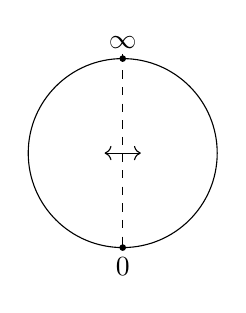
\begin{tikzpicture}[scale=0.6]
  % Draw the circle
  \draw (0,0) circle [radius=2cm];

  % Draw the points on top and bottom
  \coordinate (top) at (0,2);
  \coordinate (bottom) at (0,-2);
  \fill (top) circle [radius=2pt];
  \fill (bottom) circle [radius=2pt];

  % Draw the dashed arrow passing through the points
  \draw[dashed] (0,2.1) -- (0,-2.1);

  % Draw the horizontal arrows passing through the center
  \draw[<->, shorten >=2pt, shorten <=2pt] (-0.5,0) -- (0.5,0);

    % Add labels at the top and bottom
  \node[above] at (top) {$\infty$};
  \node[below] at (bottom) {$0$};
\end{tikzpicture}
\]
This is simply the circle with the $C_2$-action given by reflection across the equator. The two marked points are the only points fixed by the $C_2$-action.

We can also consider the regular representation $\rho$. This is a two dimensional representation, and so the underlying space is a 2-sphere. We can think of it as the one point complexification of $\mathbb{C}$, also known as $\mathbb{C}P^1$, equipped with the complex conjugation action. Since $\mathbb{R} \subseteq \mathbb{C}$ is fixed by conjugation, we see that $\mathbb{R}P^1 \subseteq \mathbb{C}P^1$ is fixed by this action. 
\[
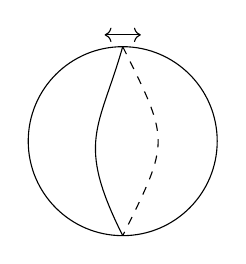
\begin{tikzpicture}[scale=0.6]
  % Draw the circle
  \draw (0,0) circle [radius=2cm];

    % Draw the points on top and bottom
  \coordinate (top) at (0,2);
  \coordinate (bottom) at (0,-2);

    % Define the control points to adjust the curve
  \coordinate (control1) at (-1,0);
    \coordinate (control3) at (-0.5,0.25);
  \coordinate (control2) at (1,0);

  % Draw the horizontal arrows passing through the center
  \draw[<->, shorten >=2pt, shorten <=2pt] (-0.5,2.25) -- (0.5,2.25);

    % Draw the curved lines
  \draw (top) .. controls (control3) and (control1) .. (bottom);
    \draw[dashed] (top) .. controls (control2) .. (bottom);
\end{tikzpicture}
\]
The  $C_2$-action is again given by reflection across an equator. 
\end{example}
\begin{notation}
Let $X$ and $Y$ be based spaces, then we let $\Map_G(X,Y) \subseteq \Map(X,Y)$ denote the space of $G$-equivariant maps $X \to Y$, with the subspace topology. Moreover, we can write define a $G$-space $G\Map(X,Y)$ to have underlying space $\Map(X,Y)$ with $G$-action given by 
\[
(g \cdot f)(x) \coloneqq g^{-1}f(gx). 
\]
The two are related: We have $G\Map(X,Y)^G = \Map_G(X,Y)$ as topological spaces, essentially by definition. 
\end{notation}
\begin{remark}
    Given a group homomorphism $H \to G$ we get a pullback functor $\phi^* \colon G\Top \to H\Top$ is the obvious way. For an injective homomorphism, this gives us restriction functors $\Res^G_H \colon G\Top \to H\Top$. This has a left and right adjoint, as we now explain. 
\end{remark}
\begin{definition}
    Let $X$ be a $H$-space, then we define a $G$-space $\Ind_H^G X = G \times_H X$ as the quotient of $G \times X$ by the relation $(g \cdot h, x) \sim (g, h \cdot x)$ for $g \in G, h \in H$. 
\end{definition}
\begin{example}
    If $H = e$ is the trivial group, then $\Ind_e^GX \cong G \times X$ is a free $G$-space. 
\end{example}
\begin{example}
    We have $\Ind_H^G(\ast) \cong G/H$. More generally, if $X$ is a space with trivial $H$-action, we have $\Ind_H^G(X) \cong X \times G/H$, where $G$ acts on $G/H$, and trivially on $X$. 
\end{example}
In analogy with Mackey functors, we have the following:
\begin{proposition}
    The functor $\Ind_H^G \colon H\Top \to G\Top$ is left adjoint to $\Res^G_H \colon G\Top \to H\Top$.
\end{proposition}
\begin{remark}
    There is a based version, which sends $X$ to $G_+ \wedge_HX $, the quotient of $G_+ \wedge X$ by the same relation as before. 
\end{remark}
\begin{remark}
    Similarly, there is a functor $\Coind_H^G \colon H\Top \to G\Top$, which sends $X$ to $\Map_H(G,X)$, the space of $H$-equivariant maps from $G$ to $X$, with $G$-action given by $(gf) \cdot g' = f(g \cdot g')$. This functor is right adjoint to restriction.

    In contrast to what we saw for Mackey functors, the left and right adjoint do not agree for spaces (we will see an example on the exercise sheet). 
\end{remark}
\begin{remark}
    In fact, given $f \colon H \to G$ a group homomorphism, the pullback functor $f^* \colon G\Top \to H\Top$ always has a left and right adjoint. Taking $G$ to be the trivial group we can get functors called fixed points and orbits, which we now explicitly define. 
\end{remark}
\begin{definition}
    For $X \in G\Top$, the fixed points $X^G$ is the subspace
    \[
    X^G = \SET{x \in X}{g \cdot x = x \text{ for all } g \in G} \subseteq X.
    \]
This defines a functor $(-)^G \colon G\Top \to \Top$, which is right adjoint to pullback along $G \to e$. 
    
    More generally, we can define $X^H$ as the composite
    \[
    G\Top \xrightarrow{\Res^G_H} H\Top \xrightarrow{(-)^H} \Top.
    \]
\end{definition}
\begin{example}
    Returning to the representation spheres considered in Example~\eqref{ex:rep-spheres} we have $(S^{\sigma})^{C_2}  = S^0$, while $(S^{\rho})^{C_2} = S^1$. 
\end{example}
\begin{definition}
   For $X \in G\Top$, the orbit of a point $x \in X$ is the set 
   \[
   G \cdot x = \SET{g \cdot x}{g \in G}
   \]
   We can define an equivalence relation on $X$ by saying that $x \sim y$ if and only if there exists a $g \in G$ such that $g \cdot x = y$. The quotient by this equivalence relation is the orbit space $X/G$ of the action. This is the left adjoint of pullback along $G \to e$. 
\end{definition}
\begin{remark}
In summary: we have
\[
\Map_G(Y,X) \simeq \Map(Y,X^G)
\]
and
\[
\Map_G(X,Y) \cong \Map(X/G,Y)
\]
where $X$ is a $G$-space and $Y$ has the trivial $G$-action. 
\end{remark}
There is an obvious notion of homotopy in equivariant homotopy. 
\begin{definition}
    Two equivariant maps $f,g \colon X \to Y$ between $G$-spaces are said to be $G$-homotopic if there is an equivariant map $h \colon I \times X \to Y$ such that $h|_{\{ 0\} \times X} \simeq f$ and $h|_{\{ 1\} \times X} \simeq g$. Here we give $I$ the trivial $G$-action. 
\end{definition}
\begin{example}
    Let % https://q.uiver.app/#q=WzAsMixbMCwwLCJcXGFzdCJdLFsxLDAsIlNee1xcc2lnbWF9Il0sWzAsMSwiXFxpbmZ0eSIsMCx7Im9mZnNldCI6LTF9XSxbMCwxLCIwIiwyLHsib2Zmc2V0IjoxfV1d
$\begin{tikzcd}[ampersand replacement=\&]
	\ast \& {S^{\sigma}}
	\arrow["\infty", shift left, from=1-1, to=1-2]
	\arrow["0"', shift right, from=1-1, to=1-2]
\end{tikzcd}$  be the inclusion of the two fixed-points of $S^{\sigma}$. Because $S^{\sigma}$ is path-connected, these are non-equivariantly homotopic. But they are not equivariantly homotopic, since the space of fixed points is not path-connected. 
\end{example}
We can now define $G$-homotopy groups, $G$-homotopy equivalences, etc. Note that by adjointness, the notion of equivariant homotopy will just be computing $\pi_n(X^G)$. Instead, it is better to remember the fixed points of all subgroups $H \le G$. To fix notation, let $\pi_n^H(X) \coloneqq \pi_n(X^H)$. 
\begin{definition}
    A morphism $f \colon X \to Y$ of $G$-spaces is a weak $G$-homotopy equivalence if the induced maps $\pi_n^H(f) \colon \pi_n^H(X) \to \pi_n^H(Y)$ are isomorphisms for all $H \le G$. 
\end{definition}
\begin{remark}
    By playing around with adjunctions we have $\pi_n^H(Y) = [G/H \times S^n,X]$, and so this leads naturally to the notion of $G$-CW-complex. 
\end{remark}
\begin{definition}
    A $G$-CW-complex is a sequential colimit of spaces $X_n$ where $X_{n+1}$ is a pushout (in $G\Top$)
% https://q.uiver.app/#q=WzAsNCxbMCwwLCJcXGNvcHJvZCBHL0ggXFx0aW1lcyBTXm4iXSxbMSwwLCJYX24iXSxbMCwxLCJcXGNvcHJvZCBHL0ggXFx0aW1lcyBEXm4iXSxbMSwxLCJYX3tuKzF9Il0sWzAsMV0sWzAsMl0sWzIsM10sWzEsM10sWzMsMCwiIiwxLHsic3R5bGUiOnsibmFtZSI6ImNvcm5lci1pbnZlcnNlIn19XV0=
\[\begin{tikzcd}[ampersand replacement=\&]
	{\coprod G/H \times S^n} \& {X_n} \\
	{\coprod G/H \times D^{n+1}} \& {X_{n+1}}
	\arrow[from=1-1, to=1-2]
	\arrow[from=1-1, to=2-1]
	\arrow[from=2-1, to=2-2]
	\arrow[from=1-2, to=2-2]
	\arrow["\ulcorner"{anchor=center, pos=0.125, rotate=180}, draw=none, from=2-2, to=1-1]
\end{tikzcd}\]
and $H$ ranges over all the subgroups of $G$. There is also a relative version where we allow $X_{-1} = A$, for some $G$-space $A$. 
\end{definition}
\begin{example}[label=ex:cell-structure-sign]
    We consider again the representation sphere $S^{\sigma}$. Here we start with the $C_2$-fixed 0-skeleton $S^0$. Here we attach a single free 1-cell $(C_2/e) \times D^1$ where one (free) endpoint is attached to $0$ and the other to the point $\infty$. 
\end{example}
\section{The $G$-Whitehead theorem}
Our next goal is to prove the equivariant Whitehead theorem.
\begin{theorem}[Equivariant Whitehead theorem]\label{thm:whitehead}
A weak $G$-homotopy equivalence between $G$-CW complexes is a $G$-homotopy equivalence. 
\end{theorem}
There are two ways to prove this theorem, both generalizing the two non-equivariant ways. The first is an inductive argument, and can be found in \cite[Theorem 2.1.31]{guillou}. The second is to prove a more general theorem, the equivariant homotopy extension and lifting property (HELP). The main subtly when extending the proof from the non-equivariant case is to define a suitable notion of the connectivity of a map. 
\begin{definition}
    Let $\theta \colon \Sub(G)/G \to \SET{x \in \bbZ}{x \ge -1}$. A map $f \colon X \to Y$ of $G$-spaces is $\theta$-connected if $f^H$ is $\theta(H)$-connected for all $H \le G$. A $G$-CW complex is $\theta$-dimensional if all cells of orbit type $G/H$ have non-equivariant dimension at most $\theta(H)$. 
\end{definition}
With these definitions in place, we now have an equivariant version of the HELP theorem.\footnote{For the details in the non-equivariant case, see \cite[Chapter 10.3]{May1999concise}.} 
\begin{proposition}
Let $(A,X)$ be a $\theta$-dimensional relative $G$-CW complex,
and let $e \colon Y \to Z$ be a $\theta$-connected $G$-map between $G$-CW complexes. Given $g \colon A \to Y$, $h \colon A \times I \to Z$, and $f \colon X \to Z$ such that $eg = hi_1$ and
$f|_A = hi_0$, there exist maps $\widetilde{g} \colon X \to Y$ and $\widetilde{h} \colon X \times I \to Z$ that make the following diagram commute:

% https://q.uiver.app/#q=WzAsOCxbMCwwLCJBIl0sWzIsMCwiQSBcXHRpbWVzIEkiXSxbNCwwLCJBIl0sWzAsMiwiWCJdLFsxLDEsIloiXSxbMiwyLCJYIFxcdGltZXMgSSJdLFs0LDIsIlgiXSxbMywxLCJZIl0sWzAsMSwiaV8wIl0sWzIsMSwiaV8xIiwyXSxbMCwzXSxbMyw0LCJmIiwyXSxbMSw0LCJoIiwyXSxbMSw1XSxbMyw1LCJpXzAiLDJdLFs2LDUsImlfMSJdLFsyLDZdLFsyLDcsImciXSxbNiw3LCJcXHRpbGRlIGciLDAseyJzdHlsZSI6eyJib2R5Ijp7Im5hbWUiOiJkYXNoZWQifX19XSxbNyw0LCJlIiwyLHsibGFiZWxfcG9zaXRpb24iOjMwfV0sWzUsNCwiXFx0aWxkZXtofSIsMix7InN0eWxlIjp7ImJvZHkiOnsibmFtZSI6ImRhc2hlZCJ9fX1dXQ==
\[\begin{tikzcd}[ampersand replacement=\&]
    A \&\& {A \times I} \&\& A \\
    \& Z \&\& Y \\
    X \&\& {X \times I} \&\& X
    \arrow["{i_0}", from=1-1, to=1-3]
    \arrow["{i_1}"', from=1-5, to=1-3]
    \arrow[from=1-1, to=3-1]
    \arrow["f"', from=3-1, to=2-2]
    \arrow["h"', from=1-3, to=2-2]
    \arrow[from=1-3, to=3-3]
    \arrow["{i_0}"', from=3-1, to=3-3]
    \arrow["{i_1}", from=3-5, to=3-3]
    \arrow[from=1-5, to=3-5]
    \arrow["g", from=1-5, to=2-4]
    \arrow["{\tilde g}", dashed, from=3-5, to=2-4]
    \arrow["e"'{pos=0.3}, from=2-4, to=2-2]
    \arrow["{\tilde{h}}"', dashed, from=3-3, to=2-2]
\end{tikzcd}\]
\end{proposition}
\begin{proof}[Sketch of proof]
The desired maps are constructed by induction on the skeleton of $X$, and then cell by cell, so we can assume that $X = G/H \times D^{n+1}$ and $A = G/H \times S^{n}$. By playing around with adjunctions, this reduces to the ordinary non-equivariant HELP theorem with $e \colon Y^H \to Z^H$, $X = D^n$ and $A = S^{n-1}$. 
\end{proof}
\begin{remark}
An equivalent way of phrasing it: under the assumption of the theorem, any diagram
% https://q.uiver.app/#q=WzAsNCxbMCwwLCJBIFxcdGltZXMgXFx7IDFcXH0iXSxbMCwxLCJBIFxcdGltZXMgSSBcXGN1cCBYIFxcdGltZXMgXFx7IDBcXH0iXSxbMSwwLCJZIl0sWzEsMSwiWiJdLFswLDEsIiIsMCx7InN0eWxlIjp7InRhaWwiOnsibmFtZSI6Imhvb2siLCJzaWRlIjoidG9wIn19fV0sWzAsMiwiZyJdLFsyLDMsImUiXSxbMSwzXV0=
\[\begin{tikzcd}[ampersand replacement=\&]
    {A \times \{ 1\}} \& Y \\
    {A \times I \cup X \times \{ 0\}} \& Z
    \arrow[hook, from=1-1, to=2-1]
    \arrow["g", from=1-1, to=1-2]
    \arrow["e", from=1-2, to=2-2]
    \arrow["{h \cup f}"',from=2-1, to=2-2]
\end{tikzcd}\]
can be completed to the diagram
% https://q.uiver.app/#q=WzAsNixbMCwwLCJBIFxcdGltZXMgXFx7IDFcXH0iXSxbMCwzLCJBIFxcdGltZXMgSSBcXGN1cCBYIFxcdGltZXMgXFx7IDBcXH0iXSxbMywwLCJZIl0sWzMsMywiWiJdLFsxLDEsIlggXFx0aW1lcyBcXHsgMSBcXH0iXSxbMSwyLCJYIFxcdGltZXMgSSJdLFswLDEsIiIsMCx7InN0eWxlIjp7InRhaWwiOnsibmFtZSI6Imhvb2siLCJzaWRlIjoidG9wIn19fV0sWzAsMiwiZyJdLFsyLDMsImUiXSxbMSwzLCJoIFxcY3VwIGYiLDJdLFswLDQsIiIsMix7InN0eWxlIjp7InRhaWwiOnsibmFtZSI6Imhvb2siLCJzaWRlIjoidG9wIn19fV0sWzQsNSwiIiwyLHsic3R5bGUiOnsidGFpbCI6eyJuYW1lIjoiaG9vayIsInNpZGUiOiJ0b3AifX19XSxbMSw1LCIiLDIseyJzdHlsZSI6eyJ0YWlsIjp7Im5hbWUiOiJob29rIiwic2lkZSI6InRvcCJ9fX1dLFs1LDMsIlxcdGlsZGUgaCIsMix7InN0eWxlIjp7ImJvZHkiOnsibmFtZSI6ImRhc2hlZCJ9fX1dLFs0LDIsIlxcdGlsZGUgZyIsMCx7InN0eWxlIjp7ImJvZHkiOnsibmFtZSI6ImRhc2hlZCJ9fX1dXQ==
\[\begin{tikzcd}[ampersand replacement=\&]
    {A \times \{ 1\}} \&\&\& Y \\
    \& {X \times \{ 1 \}} \\
    \& {X \times I} \\
    {A \times I \cup X \times \{ 0\}} \&\&\& Z
    \arrow[hook, from=1-1, to=4-1]
    \arrow["g", from=1-1, to=1-4]
    \arrow["e", from=1-4, to=4-4]
    \arrow["{h \cup f}"', from=4-1, to=4-4]
    \arrow[hook, from=1-1, to=2-2]
    \arrow[hook, from=2-2, to=3-2]
    \arrow[hook, from=4-1, to=3-2]
    \arrow["{\tilde h}"', dashed, from=3-2, to=4-4]
    \arrow["{\tilde g}", dashed, from=2-2, to=1-4]
\end{tikzcd}\]
\end{remark}
\begin{theorem}
Let $X$ be a $G$-CW complex and let $e \colon Y \to Z$ be a $\theta$-connected map between $G$-CW complexes, then 
\[
e_* \colon [X,Y]_G \to [X,Z]_G
\]
is a bijection if $\dim(X) \le \theta$ and surjective if $\dim X = \theta$. In particular, if $e$ is a weak equivalence and $X$ is any $G$-CW complexes, then $e_*$ is a bijection. 
\end{theorem}
\begin{proof}
Taking $A = \emptyset$ gives a map $\tilde g \colon X \to Y$ and a homotopy $\tilde h \colon X \times I \to Z$ satisfying $h(-,0) = f$ and $h(-,1) = e \circ \tilde g$, hence $[f] = [e \circ \tilde g] \in [X,Z]_G$ and therefore $e_*$ is surjective. Now assume we are given two maps $g_0,g_1 \colon X \to Y$ and an equivalence $[e \circ g_0] = [e \circ g_1]$. In particular, there exists a $G$-homotopy $H \colon X \times [0,1] \to Z$. 

We want to apply HELP to the pair $(X \times [0,1],X \times \{0,1\})$. We define $g \colon X \times \{ 0, 1 \} \to Y$ to be $g_0$ at time 0, and $g_1$ at time 1. Similarly, we define $h \colon X \times \{0,1\} \times I \to Z$ to be a constant homotopy. The HELP theorem then gives us a $G$-homotopy $\tilde g$ between $g_0$ and $g_1$. 
\end{proof}
As a corollary, we obtain an equivariant version of Whitehead's theorem. 
\begin{corollary}
Any $\theta$-connected $G$-map $e \colon Y \to Z$ between $G$-CW complexes of dimension less than $\theta$ is a $G$-homotopy equivalence. In particular, if $e$ is a weak equivalence, then it is a $G$-homotopy equivalence. 
\end{corollary}
\begin{proof}
A map $f \colon Z \to Y$ such that $e_*[f] = \text{id}$ is a homotopy inverse to $e$. 
\end{proof}
\begin{remark}
Using the equivariant version of HELP, one can also prove equivariant versions of cellular approximation and $G$-CW approximation. 
\end{remark}
\section{Elmendorf's theorem}
An abstract way to `do' homotopy theory in a category is to put a model structure on it. In case you haven't seen these before, we will briefly state the definitions:

 
\begin{definition}
A weak factorization system (WFS) on a category $\mathcal{C}$ is a pair $(\mathcal{L}, \mathcal{R})$ of classes of morphisms of $\mathcal{C}$ such that:
\begin{itemize}
    \item Every morphism $f \colon X \to Y$ of $\mathcal{C}$ may be factored as the composition of a morphism in $\mathcal{L}$ followed by one in $\mathcal{R}$:
    \[
    f \colon X \xrightarrow{\in \mathcal{L}} Z \xrightarrow{\in \mathcal{R}} Y.
    \]
    \item The classes are closed under having the lifting property against each other:
    \begin{itemize}
        \item $\mathcal{L}$ is precisely the class of morphisms having the left lifting property against every morphism in $\mathcal{R}$.
        \item $\mathcal{R}$ is precisely the class of morphisms having the right lifting property against every morphism in $\mathcal{L}$.
    \end{itemize}
    % https://q.uiver.app/#q=WzAsNCxbMCwwLCJ7fSJdLFswLDEsInt9Il0sWzEsMCwie30iXSxbMSwxLCJ7fSJdLFswLDEsInUiLDJdLFswLDIsImUgXFxpbiBcXG1hdGhjYWx7TH0iXSxbMiwzLCJ2Il0sWzMsMSwidyBcXGluIFxcbWF0aGNhbHtSfSJdLFsyLDEsIm0iLDIseyJzdHlsZSI6eyJib2R5Ijp7Im5hbWUiOiJkb3R0ZWQifX19XV0=
\[\begin{tikzcd}
	{{}} & {{}} \\
	{{}} & {{}}
	\arrow["u"', from=1-1, to=2-1]
	\arrow["{e \in \mathcal{L}}", from=1-1, to=1-2]
	\arrow["v", from=1-2, to=2-2]
	\arrow["{w \in \mathcal{R}}", from=2-2, to=2-1]
	\arrow["m"', dotted, from=1-2, to=2-1]
\end{tikzcd}\]
\end{itemize}
\end{definition}

\begin{definition}[Model Structure]
A model structure on a category $\mathcal{C}$ is a choice of three distinguished classes of morphisms: cofibrations $\mathcal{C}$, fibrations $\mathcal{F}$, and weak equivalences $\mathcal{W}$, satisfying the following conditions:
\begin{itemize}
    \item $\mathcal{W}$ contains all isomorphisms and is closed under two-out-of-three: given a composable pair of morphisms $f$ and $g$, if two out of the three morphisms $f$, $g$, $g \circ f$ are in $\mathcal{W}$, then so is the third.
    \item $(\mathcal{C}, \mathcal{F} \cap \mathcal{W})$ and  $(\mathcal{C} \cap \mathcal{W}, \mathcal{F})$ are two weak factorization systems on $\mathcal{C}$. The morphisms $\mathcal{F} \cap \mathcal{W}$ are called acyclic fibrations while those in $\mathcal{C} \cap \mathcal{W}$ are called acyclic cofibrations.
\end{itemize}
When a category $\mathcal{C}$ is a complete and cocomplete category with a model structure, we call it a model category.
\end{definition}
\begin{notation}
    Some more terminology: An object is cofibrant if the unique morphism $\emptyset \to X$ from the initial object is a cofibration, and is fibrant if the unique morphism $X \to \ast$ is a fibration.\footnote{If $\mathcal C$ is a model category, then it has an initial object, the colimit of the empty
diagram, and a terminal object, the limit of the empty diagram.}

The homotopy category $\Ho(\mathcal{C})$ of a model category is the universal way of inverting the weak equivalences in $\mathcal{C}$: $\Ho(\mathcal{C}) \coloneqq \mathcal{C}[\mathcal{W}^{-1}]$. 
\end{notation}
\begin{remark}
    This definition of homotopy category does not depend on the choice of fibrations and cofibrations. It only depends on the underlying category with weak
equivalences. However, the model structure makes the homotopy category easier to handle. In fact, with a model structure, the homotopy category is equivalent to the category whose objects are those which are both fibrant and cofibrant, and morphisms are the equivalence classes of morphism under left homotopy. This definition of homotopy category avoids the set theory technical issues one may meet with while doing localization.
\end{remark}

\begin{remark}
The axioms for a model category are over-determined. Indeed, one can show that a map is a cofibration (a trivial cofibration) if and only if it has the left lifting property with respect to all trivial fibrations (fibrations). Dually, a map is a fibration (a  trivial fibration) if and only if it has the right lifting property with respect to all trivial cofibrations (cofibrations). In particular, we only need to specify the weak equivalences and (co)fibrations, and then the remaining class is formally determined. 
\end{remark}
\begin{example}
    The category $\Top$ of topological spaces has a model structure with fibrations as Serre fibrations, equivalences are the weak homotopy equivalences, and  cofibrations are the retracts of relative cell complexes. We denote this by $\Top_{\Quillen}$. 

    The category $\Sets$ of sets has exactly 9 model structures on it!
\end{example}

\begin{definition}
  Suppose that $\mathcal{C}$ and $\mathcal{D}$ are model categories. We say that a pair $F \colon \mathcal{C} \leftrightarrows \mathcal{D} \colon U$ of adjoint functors with $F$ the left adjoint is a Quillen adjunction if the following equivalent conditions are satisfied:
\begin{itemize}
    \item $F$ preserves cofibrations and acyclic cofibrations;
    \item $U$ preserves fibrations and acyclic fibrations;
    \item $F$ preserves cofibrations and $U$ preserves fibrations;
    \item $F$ preserves acyclic cofibrations and $U$ preserves acyclic fibrations.
\end{itemize}  
\end{definition}
\begin{definition}
Let $\mathcal{C}$  and $\mathcal{D}$ be model categories equipped with a Quillen adjunction $F \colon \mathcal{C} \leftrightarrows \mathcal{D} \colon U$. Then we say that $\mathcal{C}$ and $\mathcal{D}$ are Quillen equivalent if the derived adjunction $F \colon \Ho(\mathcal C) \leftrightarrows \Ho(\mathcal D) \colon U$ is an equivalence of categories. This is equivalent to the following condition:
\begin{itemize}
    \item For any cofibrant $X \in \mathcal{C}$ and fibrant $Y \in \mathcal{D}$, $FX \to Y$ is a weak equivalence if and only if the adjoint $X \to UY$ is an equivalence. 
\end{itemize}
\end{definition}
 \begin{example}
     There is a model structure (the Kan model structure) on simplicial sets, where a morphism $f \colon X \to Y$ is 
      \begin{itemize}
        \item cofibration if it is a monomorphism (i.e., a level-wise injection).
        \item weak equivalence if its geometric realization is a weak equivalence in $\Top$. 
    \end{itemize}
    Then there is a Quillen equivalence
    \[
    |-| \colon \sSet_{\Kan} \leftrightarrows \Top_{\Quillen} \colon S(-)
    \]
    given by geometric realization and singular functors. 
 \end{example}
 \begin{proposition}\label{prop:model-gtop}
    There is a model structure on $G\Top$ where a map $f \colon X \to Y$ is a 
    \begin{itemize}
        \item fibration if $f^H \colon X^H \to Y^H$ is a fibration for all $H \le G$.
        \item weak equivalence if $f^H \colon X^H \to Y^H$ is a weak equivalence for all $H \le G$. 
    \end{itemize}
\end{proposition}
Elmendorf's theorem relates this to the category of presheaves on the orbit category. 
\begin{definition}
    The orbit category of a finite group $\mathcal{O}_G$ is the category whose objects are the orbits $G/H$ for $H \le G$ a subgroup, and whose morphisms are the $G$-equivariant continuous functions. Equivalently, this is the full subcategory of $G\Top$ on the objects $G/H$. 
\end{definition}
\begin{remark}
    It is useful to note that $\Hom_{\mathcal{O}_G}(G/H,G/K)$ is non-zero if $H$ is subconjugate in $G$ to $K$. Moreover, the automorphism group of $G/H$ is exactly the Weyl group, $W_G(H)$. 
\end{remark}
\begin{example}
    When $G = C_2$, the orbit category is the following category:
% https://tikzcd.yichuanshen.de/#N4Igdg9gJgpgziAXAbVABwnAlgFyxMJZABgBpiBdUkANwEMAbAVxiRAGEB9AJgHpWAvqXSZc+QijIBGKrUYs2XPkpADZMKAHN4RUADMAThAC2SMiBwQkUofqOnE5y2eoMIENESkAOMnsZwMLIMdABGMAwACqJ4BGwGWJoAFjiqFAJAA
\[
\begin{tikzcd}
C_2/e \arrow[d] \arrow[loop, distance=2em, in=125, out=55,"C_2"'] \\
C_2/C_2                                           
\end{tikzcd}
\]
\end{example}
\begin{proposition}\label{prop:model-functor}
    There is a model structure on $\Fun(\mathcal{O}_G^{op},\Top)$ where the weak equivalences and fibrations are taken objectwise. 
\end{proposition}
\begin{lemma}\label{lem:elmendorf-adjunction}
    There is an adjunction
    \[
    \theta \colon \Fun(\mathcal{O}_G^{op},\Top) \leftrightarrows G\Top \colon \psi 
    \]
    where $\theta$ is evaluation at $G/e$ and $\psi(X)(G/H) = X^H$. 
\end{lemma}
\begin{proof}[Sketch of proof]
    We show this by constructing a unit and a counit. We first note that $\theta \circ \psi(X) = X^e$, and this comes with a $G$-action (by functoriality) that agrees with the original $G$-action. We can then take the counit $\epsilon \colon \theta \circ \psi \to \text{id}$ to be the identity. 
    
  For the unit, note that for any $T \colon \mathcal{O}_G^{op} \to \Top$ and subgroups $K \le H \le G$, the map $T(G/H) \to T(G/K)$ factors through the fixed points $T(G/K)^H$. We then have
  \[
  (\psi \circ \theta (T))(G/H) = (\psi T(G/e))(G/H) = T(G/e)^H,
  \]
  and the factorization of the map $T(G/H) \to T(G/e)$ through $T(G/e)^H$ defines $\eta$. It is then straightforward to check the unit and counit identities. 
\end{proof}
\begin{remark}
    Since the counit is an equivalence, the right adjoint is fully-faithful. 
\end{remark}
\begin{theorem}[Elmendorf's theorem]
    The adjunction of \Cref{lem:elmendorf-adjunction} is a Quillen equivalence with respect to the model structures of \Cref{prop:model-gtop,prop:model-functor}.
\end{theorem}
\begin{proof}[Sketch of proof]
    We first show that the adjunction is Quillen. But this is straightforward: the functor $\psi$ preserves fibrations and weak equivalences essentially by definition.

    Now in general, the unit of the adjunction of \Cref{lem:elmendorf-adjunction} is not an equivalence. But we claim that it is for any $\mathcal X$ that is cofibrant. Indeed, one can explicitly check that the cofibrant objects in the model structure on $\Fun(\mathcal{O}_G^{op},\Top)$ are retracts of the cellular objects, and these are generated under pushouts along inclusions and directed colimits by 
    \[
\SET{\Map_G(-,G/H) \times X}{H \subseteq G, X \text{ is a cell in } \Top}
    \]
    Now in general the fixed point functors $(-)^H$ do not preserve colimits, but one can show that they do preserve retracts, pushouts and directed colimits. One can then directly check the claim from the following sequence of equivalences:
    \[
    \mathcal X(G/K) = \Map_G(G/K,G/H) \times Y = (G/H)^K \times Y = (G/H \times Y)^K = \mathcal{X}(G/e)^K
    \]

    Now suppose we are given a morphism $f \colon \theta(\mathcal X) \to \mathcal Y$ in $G\Top$ (note that in fact every object in $G\Top$ is fibrant). We can factor the $H$-fixed points of the adjoint $g^H \colon \mathcal{X}(G/H) \to \psi(\mathcal Y)^H = \mathcal{Y}^H$ as
    \[
    \mathcal{X}(G/H) \xrightarrow[\cong]{\eta_{G/H}} \mathcal{X}(G/e)^H \xrightarrow{f^H} Y^H.
    \]
    By the 2 out of 3 axiom, we see that $g^H$ is an equivalence if and only if $f^H$ is an equivalence. By the definition of the model structures, we deduce that $g$ is an equivalence if and only if $f$ is an equivalence, as required. 
\end{proof}
\begin{remark}
    Elmendorf's original theorem was only a statement about homotopy categories. More specifically, one defines a homotopy inverse to $\psi$ by using the bar construction. 
\end{remark}
\begin{remark}
    Here is an application. Let $\mathcal{F}$ be a family of subgroups (i.e., a collection closed under taking subgroups and conjugations). Then we can construct a $G$-space determined by the property that
    \[
    E\mathcal{F}^K = \begin{cases}
        \ast &\text{ if } K \in \mathcal{F} \\
        \emptyset &\text{ if } K \not \in \mathcal{F}.
    \end{cases}
    \]
    Indeed, simply define $E\mathcal{F}'$ to be the presheaf with the analogous property, and define $E\mathcal{F}$ to be the image under the Quillen equivalence. 
\end{remark}
\chapter{Forms of equivariant cohomology}
There are several different flavors of cohomology for equivariant homotopy. We begin with Borel (co)homology, before moving on to the more powerful Bredon (co)homology. 
\section{Borel cohomology}
The simplest, and perhaps most common, form of equivariant cohomology is known as Borel equivariant cohomology. 

The following can always be constructed, for example using the Milnor construction. 
\begin{definition}
    For any group $G$, we let $EG$ denote a $G$-CW complex whose underlying space is contractible, and such that the action of $G$-is free. We let the orbit space $EG/G$ be denoted by $BG$. This is known as the classifying space of the group $G$. 
\end{definition}
\begin{example}
    Let $G = C_2$ then a model for $EC_2$ is $S^{\infty}$ with the antipodal action. Here we have $S^{\infty}/C_2 \simeq \mathbb{R}P^{\infty}$, and so $BC_2 \simeq \mathbb{R}P^{\infty}$. 

    More generally, taking the limit of the inclusion of the unit sphere $S^{2n-1} \subseteq \mathbb{C}^n$, we can think of $S^{\infty}$ as the unit sphere inside of $\mathbb{C}^{\infty}$. We can think of $C_n$ as acting on each complex coordinate as multiplication by an $n$-th root of unity. This gives a free action of $C_n$ on $S^{\infty}$, and so $EC_n \simeq S^{\infty}$. We deduce that $BC_n \simeq S^{\infty}/C_n$. This is known as an infinite-dimensional lens space.  
\end{example}
\begin{remark}
    It is a good exercise to check that $EG \times EH \simeq E(G \times H)$. In particular, we deduce that $B(G \times H) \simeq BG \times BH$. 
\end{remark}
\begin{proposition}
    The space $BG$ is a $K(G,1)$, i.e., $\pi_1(BG) \simeq G$ and all other homotopy groups are trivial. 
\end{proposition}
\begin{proof}
    This follows from the fact that $G \to EG \to BG$ is a fibration, and the long exact sequence in homotopy. 
\end{proof}
\begin{definition}
    Give a $G$-space $X$, the \emph{Borel construction} on $X$ is the orbit space of the diagonal $G$-action on $EG \times X$. This is usually denoted $EG \times_G X$. The Borel equivariant homology and cohomology are defined by
    \[
    H_*^{Borel}(X) \coloneqq H_*(EG \times_G X) \quad \text{ and } \quad H^*_{Borel}(X) \coloneqq H_*(EG \times_G X). 
    \]
\end{definition}
\begin{remark}
    When compared with Bredon cohomology, this is much easier to compute. On the other hand, it can't tell the difference between $EG$ and a point. More generally, we have the following:
\end{remark}
\begin{definition}
    A map $f \colon X \to Y$ of $G$-spaces is an underlying equivalence if it induces an equivalence on underlying spaces. 
\end{definition}
The following follows essentially by definition (check on fixed points!):
\begin{proposition}
    The functor $EG \times (-) \colon G\Top \to G\Top$ takes underlying equivalences to $G$-equivalences. Therefore, Borel cohomology takes underlying equivalences to cohomology isomorphisms. 
\end{proposition}
\begin{remark}
    Taking $X$ to be a point, we see that
    \[
    H_*^{Borel}(\ast) = H_*(BG) \quad \text{ and }     H^*_{Borel}(\ast) = H^*(BG).
    \]
    It is either a theorem, or a definition, that this is the group (co)homology of the group $G$. 
\end{remark}
\section{Bredon cohomology}
There is a more refined version of equivariant cohomology known as Bredon cohomology. We need the following definition:
\begin{definition}
Let $G$ be a finite group, then a \emph{coefficient system} is a presheaf $X \in \Fun(\mathcal{O}_G^{op},\Ab)$.
\end{definition}
Note that Elemendorf's theorem says that for any coefficient system we can produce an Eilenberg--MacLane $G$-space. 
\begin{example}
Any Mackey functor $\underline{M}$ gives rise to a coefficient system by forgetting the data of the transfer map. Strictly speaking, given our definition of Mackey functors, this is not entirely obvious: one needs to note that any $G$-map $\phi \colon G/H \twoheadrightarrow G/K$ can be factored (not uniquely) as a composite $G/H \twoheadrightarrow G/K^\gamma \cong G/K$ where $H$ is contained in the conjugate $K^{\gamma}$. Then the map $M(\phi) \colon M(G/K) \to M(G/H)$ is defined by to 
\[
\underline{M}(K) \xrightarrow{c_{\gamma}} \underline{M}(K^{\gamma}) \xrightarrow{R_H^{K^{\gamma}}} \underline{M}(H).
\]
One can check that the composite does not depend on the choice of factorization. 
\end{example}
\begin{example}
For $n \ge 2$ the equivariant homotopy groups $\pi_n(X^H)$ for $H \le G$ assemble into a coefficient system denoted $\underline{\pi}_n(X)$. Indeed, the functor $G/H \mapsto X^H$ defines a coefficient system valued in (based) spaces, and then we simply apply $\pi_n$ to this. This clearly applies in other contexts, for example the assignment $\underline{H}_n(X;A)(G/H) \coloneqq H_n(X^K;A)$ determines a coefficient system. 
\end{example}
\begin{example}
Let $G = C_2$ and $X = S^{\sigma}$. Then $X^{C_2} \simeq S^0$ and $X^1 \simeq S^1$. It follows that 
% https://q.uiver.app/#q=WzAsNixbMCwxLCJcXHVuZGVybGluZXtIfV8wKFNee1xcc2lnbWF9O1xcYmJaKVxcY29uZyJdLFsxLDAsIlxcYmJaXjIiXSxbMSwyLCJcXGJiWiJdLFszLDEsIlxcdW5kZXJsaW5le0h9XzEoU157XFxzaWdtYX07XFxiYlopXFxjb25nIl0sWzQsMCwiMCJdLFs0LDIsIlxcYmJaX3tcXHNnbn0iXSxbMSwyLCJcXG5hYmxhIl1d
\[\begin{tikzcd}[row sep=0.01in,column sep=0.01in,ampersand replacement=\&]
    \& {\bbZ^2} \&\&\&\& 0 \\
    {\underline{H}_0(S^{\sigma};\bbZ)\cong} \&\&\& \quad \& {\underline{H}_1(S^{\sigma};\bbZ)\cong} \\
    \& \bbZ \&\&\&\& {\bbZ_{\sgn}}
    \arrow["\nabla", from=1-2, to=3-2]
\end{tikzcd}\]
Here we have written $\bbZ_{\sgn}$ for $\underline{H}_1(S^{\sigma})(C_2/e)$ since the nontrivial element of $C_2$ acts as an orientation-reversing map on $S^{\sigma}$.
\end{example}
\begin{example}[label=ex:cell-coefficient]
Here is an important example: for a $G$-CW complex $X$, the functor that sends $G/K$ to $C_n^{cell}(X^K)$ defines a coefficient system denoted $\underline{C_n}(X)$. This relies on the observation that the $H$-fixed points of a $G$-CW complex inherit a CW-structure. 
\end{example}
\begin{example}[label=ex:sign-sphere-cell-complex]
We constructed a cell structure on $S^{\sigma}$ in Example~\eqref{ex:cell-structure-sign}. On fixed points this gives $S^0$, with two 0-cells and no higher cells, while on the underlying space it gives the cell structure for $S^1$ with two 0-cells and two 1-cells. Then:
\[\begin{tikzcd}[row sep=0.01in,column sep=0.01in,ampersand replacement=\&]
    \& {\bbZ^2} \&\&\&\& 0 \\
    {\underline{C}_0(S^{\sigma};\bbZ)\cong} \&\&\& \quad \& {\underline{C}_1(S^{\sigma};\bbZ)\cong} \\
    \& \bbZ^2 \&\&\&\& {\bbZ[C_2]}
    \arrow["\text{id}", from=1-2, to=3-2]
\end{tikzcd}\]
Here we write $\bbZ[C_2]$ for $\underline{C}_1(S^{\sigma})(C_2/e)$ since the $C_2$-action exchanges the two 1-cells in $(S^{\sigma})^e$.
\end{example}
\begin{definition}
    A map of $G$-coefficient systems $C \to D$ is a natural transformation. We will write $\Hom_{\coeff}(C,D)$ for the set (actually abelian group) of maps between $C$ and $D$. 
\end{definition}
\begin{remark}
    If we fix a subgroup $K$ and allow $n$ to vary in Example~\eqref{ex:cell-coefficient}, then $\underline{C}_*(X) = C_*^{cell}(X^K)$ is a chain complex. The differentials commute with restriction and conjugation in the obvious manner, and so we have maps
    \[
d_n \colon \underline{C}_n(X) \to \underline{C}_{n-1}(X)    
    \]
    of coefficient systems, which make $\underline{C}_*(X)$ into a chain complex. 
\end{remark}
\begin{definition}[Bredon cohomology]
    Let $X$ be a $G$-space, and $M$ a $G$-coefficient system. $\Hom_{coeff}(\underline{C}_*(X),M)$ is a cochain complex of abelian groups, which we write $C^*_{\coeff}(X;M)$, and the \emph{Bredon cohomology} of $X$ with coefficients in $M$ is 
    \[
    H_G^n(X;M) \coloneqq H^n(C^*_{\coeff}(X;M)). 
    \]
\end{definition}
In the case of $M = \underline{\bbZ}$, this turns out to be very simple. 
\begin{lemma}\label{lem:coefficient-hom-z}
    Let $C$ be a $G$-coefficient system, then 
    \[
    \Hom_{\coeff}(C,\underline{\bbZ}) \cong \Hom_{AbGrps}(C(G/e)/G,\mathbb{Z}).
    \]
\end{lemma}
\begin{proof}Exercise.
\end{proof}
\begin{comment}
\begin{proof}[Sketch of proof:]
    Given a morphism of coefficient systems $C \to \mathbb{Z}$, we can evaluate at $G/e$ to get a map $C(G/e) \to \bbZ$, which factors through $C(G/e)/G$ because the action on $\mathbb{Z}(G/e) = \mathbb{Z}$ is trivial.  In the other direction, any morphism $C(G/K) \to C(G/e)$ must make the following diagram commute: 
    % https://q.uiver.app/#q=WzAsNCxbMCwwLCJDKEcvSykiXSxbMCwxLCJDKEcvZSkiXSxbMSwwLCJcXG1hdGhiYntafSJdLFsxLDEsIlxcbWF0aGJie1p9Il0sWzAsMV0sWzAsMiwiZl9LIiwyXSxbMiwzLCIiLDIseyJsZXZlbCI6Miwic3R5bGUiOnsiaGVhZCI6eyJuYW1lIjoibm9uZSJ9fX1dLFsxLDMsImZfZSIsMl1d
\[\begin{tikzcd}[ampersand replacement=\&]
	{C(G/K)} \& {\mathbb{Z}} \\
	{C(G/e)} \& {\mathbb{Z}}
	\arrow[from=1-1, to=2-1]
	\arrow["{f_K}", from=1-1, to=1-2]
	\arrow[Rightarrow, no head, from=1-2, to=2-2]
	\arrow["{f_e}"', from=2-1, to=2-2]
\end{tikzcd}\]
and so $f_K$ is determined by $f_e$. 
\end{proof}
\end{comment}
\begin{example}
    In Example~\eqref{ex:sign-sphere-cell-complex} we computed the cellular complex for $S^{\sigma}$, up to determining the boundary maps. There is only one map left to determine, and that is the map
    \[
    \bbZ[C_2] \cong \underline{C}_1(S^{\sigma})(C_2/e) \to \underline{C}_0(S^{\sigma})(C_2/e) \cong \mathbb{Z} \oplus \mathbb{Z}. 
    \]
    Recall that the differential of a 1-cell is just the signed sum of its two boundary 0-cells:
    \[
    d(e) = \phi(1) - \phi(0)
    \]
    for $\phi \colon S^0 \to X^0$ the attached map. In other words, $\underline{C}_*(S^{\sigma})$ is
    % https://q.uiver.app/#q=WzAsNCxbMCwwLCIwIl0sWzEsMCwiXFxtYXRoYmJ7Wn0gXFxvcGx1cyBcXG1hdGhiYntafSJdLFsxLDEsIlxcbWF0aGJie1p9IFxcb3BsdXMgXFxtYXRoYmJ7Wn0iXSxbMCwxLCJcXG1hdGhiYntafVtDXzJdIl0sWzAsMV0sWzEsMiwiXFx0ZXh0e2lkfSJdLFswLDNdLFszLDJdXQ==
\[\begin{tikzcd}[ampersand replacement=\&]
	0 \& {\mathbb{Z} \oplus \mathbb{Z}} \\
	{\mathbb{Z}[C_2]} \& {\mathbb{Z} \oplus \mathbb{Z}}
	\arrow[from=1-1, to=1-2]
	\arrow["{\text{id}}", from=1-2, to=2-2]
	\arrow[from=1-1, to=2-1]
	\arrow[from=2-1, to=2-2,"{\begin{psmallmatrix} 1 & -1 \\ 1 & -1 \end{psmallmatrix}}"']
\end{tikzcd}\]
Now we want to apply $\Hom_{coeff}(-,\underline{\mathbb{Z}})$. By \Cref{lem:coefficient-hom-z} this is
\[
\mathbb{Z} \oplus  \mathbb{Z} \xrightarrow{{\begin{psmallmatrix} 1 & -1 \end{psmallmatrix}}} \mathbb{Z}
\]
Hence,
\[
H_{C_2}^i(S^{\sigma};\underline{\mathbb{Z}}) \cong \begin{cases}
    \mathbb{Z} & i = 0 \\
    0 & \text{otherwise.}
\end{cases}
\]
\end{example}
\begin{example}
    Let us do the case $S = S^{2\sigma}$. This is the 2-sphere with action given by rotation by a half-turn. This has a $C_2$-CW structure given by the following:
    \begin{enumerate}
        \item There are two-zero cells corresponding to the two-fixed points, the north and south poles. 
        \item There is a single free one-cell corresponding to the boundary of the hemispheres. 
        \item There is a single 2-cell. 
    \end{enumerate}
    See \Cref{s2-sign}. We can then produce the cellular chain complex:
% https://q.uiver.app/#q=WzAsNixbMCwwLCIwIl0sWzEsMCwiMCJdLFsyLDAsIlxcYmJaIFxcb3BsdXMgXFxiYloiXSxbMCwxLCJcXGJiWltDXzJdIl0sWzEsMSwiXFxiYlpbQ18yXSJdLFsyLDEsIlxcYmJTIFxcb3BsdXMgXFxiYloiXSxbMiw1LCJcXHRleHR7aWR9Il0sWzEsMl0sWzQsNV0sWzEsNF0sWzAsMV0sWzAsM10sWzMsNF1d
\[\begin{tikzcd}[ampersand replacement=\&]
	0 \& 0 \& {\bbZ \oplus \bbZ} \\
	{\bbZ[C_2]} \& {\bbZ[C_2]} \& {\bbZ \oplus \bbZ}
	\arrow["{\text{id}}", from=1-3, to=2-3]
	\arrow[from=1-2, to=1-3]
	\arrow[from=2-2, to=2-3,"{\begin{psmallmatrix} 1 & -1 \\ 1 & -1 \end{psmallmatrix}}"']
	\arrow[from=1-2, to=2-2]
	\arrow[from=1-1, to=1-2]
	\arrow[from=1-1, to=2-1]
	\arrow[from=2-1, to=2-2, "1-g"']
\end{tikzcd}\]
where $C_2 = \langle g \rangle$. Applying $\Hom_{\coeff}(-,\bbZ)$  we get the chain complex
\[
\mathbb{Z} \oplus  \mathbb{Z}  \xrightarrow{{\begin{psmallmatrix} 1 & -1 \end{psmallmatrix}}} \mathbb{Z} \xrightarrow{0}\mathbb{Z}
\]
and so
\[
H^i_{C_2}(S^{2\sigma};\underline{\mathbb{Z}}) \cong \begin{cases}
    \bbZ & i = 0,2 \\
    0 & \text{otherwise.}
\end{cases}
\]
\end{example}

\begin{figure}    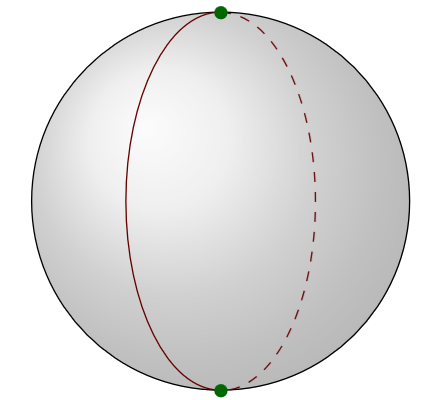
\includegraphics[width=0.5\textwidth]{s2.png}\caption{$C_2$-CW structure on $S^{2\sigma}$, the 2-sphere with a $C_2$-action by rotation through 180\textdegree.
The two green dots are the two 0-cells $C_2/C_2 \times D^0$; the red circle is the single 1-cell $C2/e \times D^1$,
and the gray hemispheres are the single 2-cell $C_2/e \times D^2$.}\label{s2-sign}. 
    \end{figure}
    Both of these could have been computed using the following general result. 
    \begin{lemma}\label{lem:bredon-constant}
        For any $G$-space $X$ we have
        \[
        H_G^i(X;\underline{\mathbb{Z}}) \cong H^i(X/G;\mathbb{Z}).
        \]
    \end{lemma}
    Indeed, in our first computation the orbit space is contractible, while in the second example, it is equivalent to $S^2$ (we have attached a two-cell to a contractible 1-skeleton). This lemma is an easy consequence of \Cref{lem:coefficient-hom-z}, but will also follow from an axiomatic treatment of equivariant cohomology theories. 

    There is also a way to get fixed points instead of orbits.
    \begin{lemma}
    For any $G$-space $X$ we have $H_G^n(X;\Inf_e^G(\bbZ)) \cong H^n(X^G;\bbZ)$. 
    \end{lemma} 
    \begin{proof}
   Exercise.
    \end{proof}
    Finally, we can also get the ordinary homology of the underlying non-equivariant space of $X$:
    \begin{lemma}
    For any $G$-space $X$, we have $H^n(X;\Ind_e^G(\bbZ)) \cong H^n(X;\bbZ)$. 
    \end{lemma}
    \begin{proof}
 This follows from the following claim: there is an equivalence \[
 \Hom_{\coeff}(C,\Ind_e^G(\bbZ)) \cong \Hom_{AbGrp}(C(e),\bbZ),\]
  which is essentially a consequence of \Cref{prop:induction-left-right-adjoint-mackey}: induction is right adjoint to the forgetful functor. 
    \end{proof}
    \begin{remark}
    There was nothing special about $\bbZ$ in these three results; we could have used any abelian group $A$. Later we will consider the case $A = \mathbb{F}_p$. 
    \end{remark}
    \section{Bredon homology}
    To define Bredon homology with need to work with functors $\mathcal{O}_G \to \Ab$ rather than $\mathcal{O}_G^{op} \to \Ab$. We call these $\mathcal{O}_G$-modules. With $M$ such an $\mathcal{O}_G$-module we define:
    \begin{definition}
    The Bredon homology of $X$ with coefficients in $M$ is
    \[
    H_n^G(X;M) \coloneqq H_n(\underline{C}_n(X) \otimes_{\mathcal{O}_G} M).
    \]
    Here $\underline{C}_n(X) \otimes_{\mathcal{O}_G} M$ denotes the coend
    \[
    \begin{split}
    \underline{C}_n(X) \otimes_{\mathcal{O}_G} M &\coloneqq \int_{}^{G/H \in \mathcal{O}_G} \underline{C}_n(X)(G/H) \otimes M(G/H).
    \end{split}
    \]
    If you haven't seen coends before, they can be given as a coequalizer: If $S \colon \cat C^{op} \times \cat C \to \cat C$ is a functor, then the coend of $S$ is equivalent to the coequalizer
    % https://q.uiver.app/#q=WzAsMyxbMCwwLCJcXGNvcHJvZF97YycgXFx0byBjfVMoYycsYykiXSxbMSwwLCJcXGNvcHJvZF97YyBcXGluIFxcY2F0IEN9UyhjLGMpIl0sWzIsMCwiXFxpbnRee1xcY2F0IEN9UyJdLFswLDEsIiIsMCx7Im9mZnNldCI6MX1dLFswLDEsIiIsMix7Im9mZnNldCI6LTF9XSxbMSwyXV0=
\[\begin{tikzcd}[ampersand replacement=\&]
   \displaystyle {\coprod_{c' \to c}S(c',c)} \& \displaystyle{\coprod_{c \in \cat C}S(c,c)} \& {\int^{c \in \cat C}S(c,c)}
    \arrow[shift right, from=1-1, to=1-2]
    \arrow[shift left, from=1-1, to=1-2]
    \arrow[from=1-2, to=1-3]
\end{tikzcd}\]
To ground your intuition, thinking of a ring as an Ab-enriched category with one object, then a left $R$-module $B$ is an additive functor $R \to Ab$ sending the one object of $R$ to the abelian group $B$ and sending each arrow $r \in R$ to the scalar multiplication $r_* \colon b \mapsto rb$. A right $R$-module is an additive functor $R^{op} \to Ab$. In particular, $R \mapsto A \otimes B$ is a bifunctor $R^{op} \times R \to Ab$. Then,
\[
\int^R A \otimes B = A \otimes_R B
\]
is the usual tensor product over $R$. 
    \end{definition}
    \begin{remark}
    One gets an $\mathcal{O}_G$-module from a Mackey functor by forgetting the \emph{restriction} maps. 
    \end{remark}
    One has analogs of the results about Bredon cohomology:
    \begin{lemma}\label{lem:bredon-homology}
    There are isomorphisms
    \begin{enumerate}[label=(\roman*)]
        \item $H_n^G(X;\underline{\mathbb{Z}}) \cong H_n(X/G;\mathbb{Z})$,
        \item $H_n^G(X;\Inf_e^G(\bbZ)) \cong H_n(X^G;\mathbb{Z})$, and 
        \item $H_n^G(X;\Ind_e^G(\bbZ)) \cong H_n(X;\mathbb{Z})$. 
    \end{enumerate}
    \end{lemma}
    \begin{remark}
    Let us relate Bredon (co)homology with Borel cohomology. We have
        \[
    H^*_{Borel}(X;\mathbb{Z}) \coloneqq H^*(EG \times_G X;\mathbb{Z})  \cong H^*(EG \times X;\underline{\mathbb{Z}})
    \]
    and
    \[
    H_*^{Borel}(X;\mathbb{Z}) \coloneqq H_*(EG \times_G X;\mathbb{Z})  \cong H_*(EG \times X;\underline{\mathbb{Z}})
    \]
    So Borel (co)homology is just a special case of Bredon (co)homology. Note then that the projection map $EG \times X \to X$ induces a map
    \[
\phi \colon H^*(X;\underline{\mathbb{Z}}) \to     H^*_{Borel}(X;\mathbb{Z})  
    \]

    \end{remark}
    \begin{lemma}
    Suppose that $X$ is a free $G$-CW complex,  i.e., it can be built from free cells $G_+ \times D^n$, then $\phi$ is an isomorphism.
    \end{lemma}
    \begin{proof}
For such spaces the projection map $EG \times X \to X$ is a $G$-equivariant weak equivalence. Since $X$ was assumed to be a $G$-CW complex, the Whitehead theorem (\Cref{thm:whitehead}) implies that the projection is a $G$-equivariant homotopy equivalence. 
    \end{proof}
    \section{Application - Smith theory and the Conner conjecture}
    We will use Bredon homology to prove the following theorem. 
    \begin{theorem}[Smith]
    Let $G$ be a finite $p$-group and $X$ be a finite $G$-CW complex such that the underlying topological space of $X$ is an $\mathbb{F}_p$-cohomology sphere, i.e.,  $H^*(X;\mathbb{F}_p) \cong H^*(S^n;\mathbb{F}_p)$ for some $n$. Then $X^G$ is either empty or an $\mathbb{F}_p$-cohomology sphere (of equal or smaller dimension).  
    \end{theorem}
    \begin{proof}
We claim that we can easily reduce to the case $G = \bbZ/p$. Indeed, if $H \subseteq G$ is a normal subgroup, then $X^G \cong (X^H)^{(G/H)}$, and so we can induct on the order of the group using the Sylow theorems. We have already seen that there exist coefficient systems $M$ and $N$ such that 
\[
H_G^*(X;M) \cong H^*(X;\bbF_p) \quad \text{ and } \quad H_G^*(X;N) \cong H^*(X^G;\mathbb{F}_p). 
\]
namely $M = \Ind_e^{G}(\bbF_p)$ and $N = \Inf_e^G(\bbF_p)$. We claim that there also exists a coefficient system $L$ such that $H_{C_p}^*(X;L) \cong \widetilde H^*((X/X^{C_p})/C_p;\mathbb{F}_p)$. Indeed, we leave it as an exercise to show that $L \coloneqq \ker(\underline{\bbF}_p \to \Inf_e^{C_p}(\bbF_p))$ works.

We now fix $p = 2$ for simplicity. We have a short exact sequence
\[
\bbF_2 \xrightarrow{\Delta} \bbF_2[C_2] \xrightarrow{\nabla} \bbF_2
\]
which extends to a short exact sequence of coefficient systems 
\[
0 \to L \to M \to N \oplus L \to 0.
\]
 This induces a long exact sequence in cohomology, which we can rewrite (using the definitions of the coefficient systems) as 
\[
\begin{split}
\cdots \to \widetilde H^n((X/X^{C_2})/C_2;\mathbb{F}_2) &\to H^n(X;\bbF_2) \to \widetilde H^n((X/X^{C_2})/C_2;\mathbb{F}_2) \oplus H^n(X^{C_2};\bbF_2) \\ &\to \widetilde H^{n+1}((X/X^{C_2})/C_2;\mathbb{F}_2) \to \cdots
\end{split}
\]
Let 
\[
a_n = \dim \widetilde H^n((X/X^{C_2})/C_2;\mathbb{F}_2), \quad b_n = \dim  H^n(X;\bbF_2), \quad c_n = H^n(X^{C_2};\bbF_2). \]
Then exactness of the long exact sequence (at the direct sum) implies that
\[
a_n + c_n \le b_n + a_{n+1}. 
\]
Note that
\[
a_0 + c_0 + c_1 \le b_0 + a_1 + c_1 \le b_0 + b_1 + a_2
\]
or more generally that 
\[
a_q + c_q + c_{q+1} + \ldots c_{q+n} \le b_q + b_{q+1} + \cdots + b_{q+n} + a_{q+n+1}
\]
for any $n$ and $q \ge 0$. Taking $q = 0$ and $n$ large enough, we deduce that $\sum c_i \le \sum b_i$. But by assumption $\sum b_i = 2$. It follows that $\sum c_i \le 2$. If we assume that $X^{C_2}$ is non-zero, then we must have $\sum c_i > 0$, so it remains to eliminate the possibility that $\sum c_i = 1$. But applying the Euler characteristic\footnote{Recall that this is the alternating sum of the ranks of the cohomology} we deduce that 
\[
\chi(X) = \chi(X^{C_2}) + 2\chi((X/X^{C_2})/C_2)\equiv \chi(X^{C_2}) \mod (2). 
\]
This finishes the proof. 
\end{proof}
 \begin{theorem}[Conner conjecture, proved by Oliver]
Let $G$ be a finite group, and let $X$ have the homotopy type of a finite dimensional $G$-CW complex. Then,
\[
\widetilde H^*(X;A) = 0 \implies \widetilde H^*(X/G;A) = 0. 
\]
 \end{theorem}
 \begin{remark}
 The finiteness assumption is necessary. Note that the free $G$-space $EG$ is contractible, but $EG/G = BG$ has non trivial cohomology unless $G = e$. 
 \end{remark}

 \begin{proof}
We will prove this for $G = C_p$ - again, once can reduce to this case. We will still stick with $p = 2$. First, we assume that $X^{C_2}$ has a fixed point - if not, we can replace it with $\Sigma X$.

 By Smith theory, and the assumption that $X$ is acyclic, we have
 \[
 \sum_i c_i = \sum_i \dim(H^i(X^{C_2};\bbF_2)) \le \sum_i b_i = \sum_i \dim(H^i(X;\bbF_2)) = 1.
 \]
and
 \[
 \chi(X) \equiv \chi(X^{C_2})  = 1 \mod (2).
 \]
This is only possible if $\widetilde H^*(X^{C_2};\bbF_2) = 0$. Likewise, summing over the inequalities,
\[
a_q+c_q \le b_q + a_{q+1}
\]
we deduce that $a_q = 0$ for all $q >0$ (this uses that $b_0 = a_0 = 1$ and $b_q = a_q = 0$ for $q>0$), so that $\widetilde H^*((X/X^{C_p})/C_p;\mathbb{F}_p) = 0$ as well. This is enough to show that $\widetilde H^*(X/C_p;\mathbb{F}_p) = 0$ as well, by using the long exact sequence of the following:
\[
X^{C_p} \hookrightarrow X/X^{C_p} \to (X/X^{C_p})/C_p
\]
Now suppose that $A = \mathbb{Q}$. Then the composite
\[
\widetilde H^*(X/C_p;\mathbb{Q}) \xrightarrow{} \widetilde H^*(X;\mathbb{Q})  \xrightarrow{\tau} \widetilde H^*(X/C_p;\mathbb{Q})
\]
where the second map is the transfer, is multiplication by $|C_p| = p$, and so is an isomorphism. It follows that $\widetilde H^*(X/C_p;\mathbb{Q}) = 0$. Now suppose that the theorem holds for $A = \mathbb{Z}$. Then by universal coefficients $\widetilde H^*(X;A) = 0$ for $A = \mathbb{Q}$ and $A = \mathbb{F}_p$, and so by the above,  $\widetilde H^*(X/C_p;A) = 0$ for $A = \mathbb{Q}$ and $A = \mathbb{F}_p$. Running universal coefficients again, the theorem holds for $A = \mathbb{Z}$, and then finally one last application of the universal coefficient theorem shows that it holds for arbitrary coefficients. 
 \end{proof}
\section{Axioms for equivariant homology and cohomology}
We know that (co)homology can be characterized on CW complexes by the Eilenberg--Steenrod axioms. Are there similar axioms for equivariant (co)homology theories? The answer is yes. This takes place in the category of pairs of $G$-CW complexes, i.e., the category with objects $(X,A)$ for $X$ a $G$-CW complex and $A$ a sub-complex, and morphisms $(X,A) \to (Y,B)$ morphisms $f \colon X \to Y$ such that $f(A) \subseteq B$. 
\begin{definition}
    A (ordinary) homology theory on $G$-CW complexes is a sequence of functors $h_n(X,A)$ on pairs of $G$-CW complexes and natural transformations $\delta \colon h_n(X,A) \to h_{n-1}(A,\emptyset)$ satisfying the following axioms:
    \begin{enumerate}[label=(\arabic*)]
        \item(Homotopy invariance) If $f \simeq g$, then $f_*   = g_*$. 
        \item(Long exact sequence) If we let $h_n(X) \coloneqq h_n(X,\emptyset)$ then there is an exact sequence
        \[
        \cdots \to h_n(A) \to h_n(X) \to h_n(X,A) \xrightarrow{\delta} h_{n-1}(A) \to \cdots 
        \]
        \item(Excision) If $X$ is the union of subcomplexes $A$ and $B$, then the inclusion $(A,A \cap B) \hookrightarrow (X,B)$ induces an isomorphism
        \[
        h_n(A,A \cap B) \cong h_n(X,B)
        \]
        \item(Additivity) If $(X,A)$ is a disjoint union of pairs $(X_i,A_i)$, then the inclusions $(X_i,A_i) \to (X,A)$ induce an isomorphism
        \[
        \bigoplus_ih_n(X_i,A) \cong h_n(X,A). 
        \]
        \item(Dimension) $h_n(G/H) = 0$ if $n \ne 0$. 
    \end{enumerate}
    For cohomology theories, reverse the directions of the arrows. 
\end{definition}
\begin{theorem}
    Bredon (co)homology is an equivariant (co)homology theory, where we set $\underline C_*(X,A) = \widetilde{\underline C}_*(X/A)$. 
\end{theorem}
\begin{proof}
    Homotopy invariant, excision and additivity and excision are relatively straightforward. Let us discuss the dimension axiom and the long exact sequence. Recall that $\underline{C}_*(X)$ is a coefficient system whose value at $(G/K)$ is the free abelian group $C_*^{cell}(X^K)$. We can do homological algebra in the category of coefficient systems, and we claim that $\underline{C}_*(X)$ is a projective object here. We will not prove this, but it is a consequence of a more general result:
    \begin{lemma}
        If $S$ is a finite $G$-set, then the coefficient system $F_S$ with 
        \[
        F_S(G/H) = F(S^H)
        \]
        the free abelian group on the set $S^H$, is a projective object in the category of coefficient systems. 
    \end{lemma}
    This lemma implies that $\Hom(\underline C_*(X),-)$ preserves short exact sequences of coefficient systems, and it follows that we get the desired long exact sequence. A Yoneda lemma argument shows that 
    \[
    H_G^0(G/H;M) \coloneqq H^0(\Hom_{\coeff}(\underline{C}_*(G/H),M)) \cong M(G/H)
    \]
    while
    \[
    H_G^i(G/H;M) \cong 0
    \]
    for $i > 0$. 
\end{proof}
\begin{remark}
    In fact, a uniqueness theorem similar to the usual theorem for non-equivariant cohomology shows that Bredon cohomology with coefficients in $M$ is the only equivariant cohomology theory with those coefficients. 
\end{remark}
\begin{remark}
    There is a spectral sequence
    \[
    \Ext^p_{coeff}(h_q(X),M) \implies H_G^{p+q}(X;M),
    \]
    where $h_q(X)(G/H) = H_q(X^H)$. 
\end{remark}
\begin{remark}[$RO(G)$-grading]
So far we have indexed our cohomology theories on the integers $\bbZ$. However, we have already seen that we have more notions of a sphere in equivariant homotopy. So, can we (and should be) grade on the group $RO(G)$? There are some subtle issues here.\footnote{For amusement, see \cite[Section 6]{MR764596}.} The point is that $RO(G)$ consists of \emph{equivalence} classes, and we really want to the remember the isomorphisms between isomorphic representations. The usual fix is to rather fix an choice of preferred representatives. For example, this is easy to do when we talk about $G = \bbZ/2$ when the representation theory is simple. We will tend to ignore this remark from now, but please be aware of it. 
\end{remark}
\begin{remark}
    With how we have defined it, Bredon cohomology is only stable in the following sense: we have
    \[
    \widetilde H^n_G(X;M) \cong \widetilde H^{n+q}_G(\Sigma^qX;M)
    \]
    for any based $G$-space $X$. 
\end{remark}
In any case, we end up with suspension and loop functors for a representation $V$, and the following axiom:
\begin{axiom}[Equivariant suspension axiom]
For each $\alpha \in RO(G)$ and actual representation $V$, there is a natural isomorphism
\[
\Sigma^V\colon \widetilde H_G^{\alpha}(X) \xrightarrow{\sim} \widetilde H_G^{\alpha+V}(\Sigma^VX) = \widetilde H_G^{\alpha+V}(S^V \wedge X).
\]
\end{axiom}
In general, even determining $\widetilde H_G^{\alpha}(G/K_+)$ for $\alpha \not \in \bbZ$ is very complicated. 
\begin{remark}
    One might wonder if Bredon cohomology with coefficients in $M$ extends to an $RO(G)$-graded cohomology theory in general. This turns out to not be true. In fact, it is a theorem of Lewis, May, and McClure that it does so if and only $M$ is the underlying coefficient system of a Mackey functor.
    \end{remark}
We will do one single computation, that of the Bredon cohomology of a point with $G = \bbZ/2$ and coefficients in the constant coefficient system $\underline{\mathbb{F}_2}$. We recall that $RO(C_2) \cong \bbZ\{ \mathbf{1} \} \oplus \bbZ\{\sigma\}$, so our groups will be bigraded. The result is best described pictorially:
\begin{theorem}
The bigraded groups $H_{C_2}^{n+k\sigma}(\ast,\ul{\mathbb{F}_2})$ are as follows:
\[
H_{C_2}^{n+k\sigma}(\ast,\ul{\mathbb{F}_2}) \cong \begin{cases}
\bbF_2 & n+k \le 0, n \ge 2, k \le -2 \\
\bbF_2 & n+k \ge 0, n \le 0, k \ge 0 \\
& \text{ else}. 
\end{cases}
\]
See \Cref{fig:eq-coh-point}.

\begin{figure}[h!]
  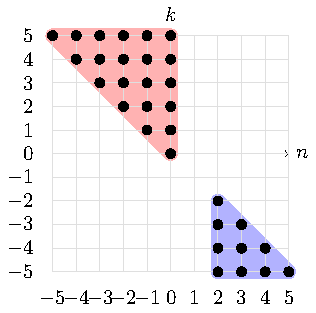
\includegraphics{sseq.pdf}
     \caption{The equivariant cohomology of a point.  Each dot represents a copy of $\bbF_2$:}\label{fig:eq-coh-point}
\end{figure}
\end{theorem}
\begin{proof}
    We will start with the blue region. These are the groups $H^{n-k\sigma}(\ast,\ul{\bbF_2})$ for $k >0$, which, using the suspension axiom becomes, 
    \[
    H_{C_2}^{n-k\sigma}(\ast,\ul{\bbF_2}) \cong \widetilde H_{C_2}^{n-k\sigma}(S^0,\ul{\bbF_2}) \cong \widetilde H_{C_2}^n(S^{k\sigma},\ul{\bbF_2}) \cong \widetilde H^n(S^{k\sigma}/C_2,\bbF_2)
    \]
    by the $\bbF_2$-analog of \Cref{lem:bredon-constant}. Let us think a little about the space $S^{k\sigma}/C_2$. When $k = 1$, this was demonstrated in Example~\eqref{ex:rep-spheres} - it is the $S^1$ with $C_2$-action given by reflection across the equator. Therefore, two points are in the same orbit if and only if they are `opposite' each other. In the orbit space, these two points get identified, and the orbit space is contractible. To consider the general case, it is useful to introduce a bit more notation. 
    \begin{definition}
        For an orthogonal representation\footnote{i.e., one that lands in $O(n)$, and $V$ is an inner product space} $V$, let 
    
        \begin{enumerate}
            \item $D(V) = \{ \mathbf{v} \in V \mid \norm{v} \le 1\}$ \\
            \item $S(V) = \{ \mathbf{v} \in V \mid \norm{v} = 1 \}$.
        \end{enumerate}
These are both unbased $G$-spaces, simply by restricting the action on $V$. 
        
Observe then that $D(V)/S(V) \cong S^V$ the one point compactification of $V$. Explicitly, this is induced by the map 
\[
D(V) \to S^V, \quad v \mapsto \begin{cases}v/(1-\norm{v}) &\text{ if } \norm{v} <1 \\
\infty &\text{ if } \norm{v} = 1.\end{cases}
\]
If the representation is trivial, this is just the usual homeomorphism $S^n \cong D^n/S^{n-1}$. Finally, if $X_+$ denotes an unbased space $X$ with a disjoint basepoint, then there is a cofibration sequence of \emph{based} $G$-spaces
\[
S(V)_+ \to D(V)_+ \to S^V
\]
    \end{definition}
   \begin{example}
       Let $G = C_2$ and $V = \sigma$, the sign representation, then $S(V) = S^0 = \bbZ/2$ with the $C_2$-action that swaps the 2-points (the 2 points correspond to 1 and -1), and there is a cofibration sequence of based $C_2$-spaces
       \[
       \bbZ/2_+ \to S^0 \to S^{\sigma}
       \]
       In general, we see that $S(k\sigma)$ is $S^{k-1}_a$, the $(k-1)$-sphere with the antipodal $C_2$-action. Passing to orbit spaces, we that that there is a sequence
       \[
       \mathbb{RP}^{k-1} \to \ast \to S^{k\sigma}/C_2
       \]
       or in other words $S^{k\sigma}/C_2 \simeq \Sigma \mathbb{RP}^{k-1}$. 
   \end{example} 

    Returning to the computation, we then see that 
    \[
    \widetilde H^n(S^{k\sigma}/C_2,\bbF_2) \cong \widetilde H^n(\Sigma \mathbb{RP}^{k-1};\mathbb{F}_2)
    \]
   These groups are given by
    \[
    \widetilde H^n(\Sigma \bbR \mathbb{P}^{k-1};\bbF_2) \cong \begin{cases} \bbF_2, & n = 2,3,\ldots,k \\ 0 & \text{else}. \end{cases}
    \]
    So, for $k > 0$, we have
    \[
    H^{n-k\sigma}(\ast;\ul{\bbF}_2) \cong \begin{cases}  \bbF_2 & 2 \le n \le k \\ 0 &\text{else}\end{cases}
    \]
    These determines the blue region of the diagram (this is often referred to as the `negative' cone). Pictorially, we are looking at a copy of $\Sigma \mathbb{R}P^{k-1}$ along a horizontal line (namely, $-k$). 

    Now we turn to the harder part, which is the computation of $ H_{C_2}^{n+k\sigma}(\ast;\ul{\bbF}_2)$ for $k\ge 0$. Here we have
    \[
    H_{C_2}^{n+k\sigma}(\ast;\ul{\bbF}_2) \cong \widetilde H_{C_2}^{n+k\sigma}(S^0;\ul{\bbF_2}) \cong \widetilde H^{C_2}_{-n-k\sigma}(S^0;\ul{\bbF}_2)
    \]
    where the last equivalence uses an equivariant version of Poincar\'{e} duality. This is in fact the motivation for $RO(G)$-grading - if we want to have Poincar\'{e} duality, we are forced into grading over representations. Taking this on faith, we must therefore compute the groups $\widetilde H^{C_2}_{-n}(S^{k\sigma},\ul{\bbF_2})$.
    Since we work with homology, the $\mathcal{O}_G$-module $\ul{\bbF}_2$ here refers to the $\mathcal{O}_G$-module whose transfer maps are all $0$. This $\mathcal{O}_G$-module splits as $\Inf_e^{C_2}\bbF_2 = N$ and $L$, the $\mathcal{O}_G$-module that is $\bbF_2$ at the bottom, and $0$ at the top. So
    \[
 \widetilde H^{C_2}_{-n}(S^{k\sigma};\ul{\bbF_2}) \cong \widetilde H^{C_2}_{-n}(S^{k\sigma};N \oplus L) 
\cong \widetilde H^{C_2}_{-n}(S^{k\sigma};N) \oplus \widetilde H^{C_2}_{-n}(S^{k\sigma};L)
    \]
    By \Cref{lem:bredon-homology} (using that $(S^{k\sigma})^{C_2} \simeq S^0$) and the homology analog of the argument given in the proof of Smith theory, we have 
    \[
     \widetilde H^{C_2}_{-n}(S^{k\sigma};\ul{\bbF_2})  \cong \widetilde H_{-n}(S^0;\bbF_2) \oplus \widetilde H_{-n}(((S^{k\sigma})/S^0)/C_2;\bbF_2)
    \]
    The first term gives us an $\bbF_2$ when $n = 0$, and gives the dots on the positive $y$-axis in the figure.  The hard part is in working out $\widetilde H_{-n}(((S^{k\sigma})/S^0)/C_2;\bbF_2)$.

    We recall that there is a cofibration
    \[
    \mathbb{RP}^{k-1}_+ \to S^0 \to {S^{k\sigma}/C^2} \to  \Sigma\mathbb{RP}^{k-1}_+
    \]
We therefore deduce that
    \[
     \widetilde H^{C_2}_{-n}(S^{k\sigma};\ul{\bbF_2})  \cong \widetilde H_{-n}(S^0;\bbF_2) \oplus \widetilde H_{-n}(\Sigma \bbR\mathbb{P}^{k-1}_+;\bbF_2)
    \]
    The first term contributes an $\bbF_2$ when $n = 0$, while the second does so whenever $n -1 \in [0, k - 1]$ or equivalently, $n \in [1,k]$. This gives the red region in the diagram. 
\end{proof}
\begin{remark}
    There are many ways to do this calculation. Let us recall that we had a cofibration of $C_2$-spaces
    \[
    C_2\to \ast \to S^{\sigma}
    \]
    which gives rise to a long exact sequence in cohomology, which we denote as follows (maps are labelled by degrees):
    % https://q.uiver.app/#q=WzAsMyxbMCwwLCJIX3tDXzJ9XntcXGFzdCtcXGFzdFxcc2lnbWF9KFNee1xcc2lnbWF9KSJdLFsyLDAsIkhfe0NfMn1ee1xcYXN0K1xcYXN0XFxzaWdtYX0oXFxhc3QpIl0sWzEsMSwiSF97Q18yfV57XFxhc3QrXFxhc3RcXHNpZ21hfShDXzIpIl0sWzAsMSwiKDAsMCkiXSxbMSwyLCIoMCwwKSJdLFsyLDAsIigxLDApIl1d
\[\begin{tikzcd}[ampersand replacement=\&]
	{H_{C_2}^{\ast+\ast\sigma}(S^{\sigma})} \&\& {H_{C_2}^{\ast+\ast\sigma}(\ast)} \\
	\& {H_{C_2}^{\ast+\ast\sigma}(C_2)}
	\arrow["{(0,0)}", from=1-1, to=1-3]
	\arrow["{(0,0)}", from=1-3, to=2-2]
	\arrow["{(1,0)}", from=2-2, to=1-1]
\end{tikzcd}\]
So what is the cohomology of $C_2$?
\begin{lemma}\label{lem:c2-cohomology}
    The Bredon cohomology $H_{C_2}^{*+*\ast}(C_2)$ is a graded commutative polynomial algebra on a generator $t \in H^{-1+\sigma}_{C_2}({C_2})$.
\end{lemma} 
\begin{proof}
    Note that, for every $G$-space $X$, we have a $G$-homeomorphism $G_+ \wedge X \simeq G_+ \wedge X_e$, where $X_e$ is $X$ with trivial $G$-action. From this, we get the chain of isomorphisms:
\[
\begin{split}
H^{a+b\sigma}_{C_2}(C_2) \xrightarrow[\cong]{\text{suspension}} \widetilde{H}^{(a+(b+n)\sigma}_G(\Sigma^{n\sigma}({C_2}_+))\xrightarrow{\cong} \\
\widetilde{H}^{a+(b+n)\sigma}_{C_2}(\Sigma^n(C_2)_+) \xleftarrow[\cong]{\text{suspension}} H^{a-n+(b+n)\sigma}_{C_2}(C_2). \end{split}
\]
This is an isomorphism of graded $H^{*+*\sigma}_{C_2}(C_2)$-modules, so it is given by multiplication by an invertible element $t_n \in H^{-n+n\sigma}_{C_2}$. In other words, the cohomology groups associated with representations of the same dimension are all isomorphic.
By the cohomology axioms, we have $H^{0+0\sigma} = \mathbb{F}_2$ and $H^{a+0\sigma}_{C_2} = 0$ if $a \ne 0$. So:
\[
\begin{cases}
 H_{C_2}^{a+b\sigma} = \mathbb{F}_2 &\text{ if } a = -b \\
 0 & \text{ else.}
\end{cases}
\qedhere
\]
\end{proof}
Returning back to the triangle above, we can use the suspension isomorphism $H_{C_2}^{\ast+\ast\sigma}(S^{\sigma}) \simeq H_{C_2}^{\ast+(\ast-1)\sigma}(\ast)$ to replace the top left corner with the cohomology of a point: 
% https://q.uiver.app/#q=WzAsMyxbMCwwLCJIX3tDXzJ9XntcXGFzdCtcXGFzdFxcc2lnbWF9KFxcYXN0KSJdLFsyLDAsIkhfe0NfMn1ee1xcYXN0K1xcYXN0XFxzaWdtYX0oXFxhc3QpIl0sWzEsMSwiSF97Q18yfV57XFxhc3QrXFxhc3RcXHNpZ21hfShDXzIpIl0sWzAsMSwiKDAsMSkiXSxbMSwyLCIoMCwwKSJdLFsyLDAsIigxLC0xKSJdXQ==
\[\begin{tikzcd}[ampersand replacement=\&]
	{H_{C_2}^{\ast+\ast\sigma}(\ast)} \&\& {H_{C_2}^{\ast+\ast\sigma}(\ast)} \\
	\& {H_{C_2}^{\ast+\ast\sigma}(C_2)}
	\arrow["{(0,1)}", from=1-1, to=1-3]
	\arrow["{(0,0)}", from=1-3, to=2-2]
	\arrow["{(1,-1)}", from=2-2, to=1-1]
\end{tikzcd}\]
The top row is given by multiplication by an element $\tau \in H_{C_2}^{\sigma}(\ast)$. Using \Cref{lem:c2-cohomology} one can see that $\tau$ is an isomorphism of groups
\[
H^{a+b\sigma}(\ast) \to H^{a+(b+1)\sigma}(\ast)
\]
except when except when $H^{a+(b+1)\sigma}(C_2)$ or $H_{C_2}^{a-1+(b+1)\sigma}(C_2)$ are non-zero. We know that $H^{0}(\ast) \cong \mathbb{F}_2$ and $H^{a}(\ast) \ne 0$ for $a \ne 0$. This gives us nearly all the zero entries that we saw in the computation before. It also tells us a little about the multiplicative structure. 

One can continue in this manner. For example, there is an exact sequence
\[
0 \to H_{C_2}^{-1+\sigma}(\ast) \to H_{C_2}^{-1+\sigma}(C_2) \to H^{0,0}(\ast) \xrightarrow{\tau} H_{C_2}^{\sigma}(\ast) \to 0
\]
This gives
\[
0 \to H_{C_2}^{-1+\sigma}(\ast) \to \bbF_2 \to \bbF_2 \to H_{C_2}^{\sigma}(\ast) \to 0
\]
One can compute that the middle map is $0$ (it is the transfer map in the Mackey functor $\mathbb{F}_2$), and so $H_{C_2}^{-1+\sigma}(\ast) \cong \mathbb{F}_2$ and $H_{C_2}^{\sigma}(\ast) \cong \mathbb{F}_2$, as we saw before. One now proceeds methodically, and gets the same answer as before. 
\end{remark}
\chapter{From $G$-spaces to $G$-spectra}
\section{From spaces to spectra}
\subsection*{Introduction to spectra}
We begin with some motivation for the category of spectra. 
\begin{remark}
    We recall that for a space $X$ the Freudenthal suspension theorem says that the maps
    \[
    \pi_n(X) \xrightarrow{\Sigma} \pi_{n+1}(\Sigma X) \xrightarrow{\Sigma}  \pi_{n+2}(\Sigma^2X) \xrightarrow{\Sigma}  \cdots
    \]
    eventually stabilize (after finitely many steps). For example, $\pi_{n+1}(S^n) \cong \mathbb{Z}/2$ for $n>2$. We call these the \emph{stable} homotopy groups of $X$. Note that these are in fact always \emph{abelian} groups. One can wonder: is there an object whose $n$-th homotopy group is the $n$-th stable homotopy groups of $X$. This is what spectra are designed to do. 
\end{remark}
\begin{definition}
    A spectrum $E$ is a sequence of based spaces $E = \{ E_n \}$ (usually graded on the natural numbers, but the story does not change if we use the integers) and structure maps $\sigma_n \colon \Sigma E_n \to E_{n+1}$. The $r$-th homotopy group of $E$ is defined to be
    \[
    \pi_r(E) \coloneqq \varinjlim_{n \to \infty} \pi_{n+r}(E_n),
    \]
    where the colimit is taken over the diagram where the maps are 
    \[
    \pi_{n+r}(E_n) \xrightarrow{\Sigma} \pi_{n+r+1}(\Sigma E_n) \xrightarrow{\sigma_{n,\ast}} \pi_{n+r+1}(E_{n+1}).
    \]
    A CW-spectrum additionally has the property that each $E_n$ is a CW-complex, and the maps $\Sigma E_n \to E_{n+1}$ exhibit $\Sigma E_n$ as a subcomplex of $E_{n+1}$. 
\end{definition}
\begin{remark}
    The homotopy groups are equivalently given by the colimit over the maps
    \[
    \pi_{n+r}(E_n) \xrightarrow{\overline{\sigma_n}_*} \pi_{n+r}(\Omega E_{n+1}) \cong \pi_{n+r+1}(E_{n+1})
    \]
\end{remark}
\begin{remark}
    We note that stable homotopy groups are in general defined for all $r \in \mathbb{Z}$, where we must start the colimit for $n+r \ge 0$. For example, $\pi_{-1}(E)$ is the colimit of 
    \[
    \pi_0(E_1) \to \pi_1(E_2) \to \cdots 
    \]
\end{remark}
\begin{example}
    For a based space $X$, the suspension spectrum $\Sigma^{\infty}X$ is the spectrum consisting of spaces $\{ \Sigma^n X\}$ with maps $\sigma_n \colon \Sigma^{n+1}X \to \Sigma^{n+1}X$ the identity map. If $X$ is a CW-space, then $\Sigma^{\infty}X$ is a CW-spectrum. For example, $\Sigma^{\infty}S^0$ is what people refer to as the \emph{sphere spectrum} and is often denoted by $\mathbb{S}$. We leave it as an exercise to show that
    \[
    \pi_n(\Sigma^{\infty}X) \cong \begin{cases}\pi_n^{\text{stable}}(X) & n \ge 0 \\ 0 & n<0 \end{cases}\]
    Note that by replacing $X$ with $\Sigma^dX$ we can product a suspended version of $\Sigma^{\infty}X$. But using spectra, we can also give an inverse to this construction: 
\end{example}
\begin{example}
    For any integer $d \ge 0$, we can created a `desuspended' suspension spectrum. Indeed, set $X_n$ to be $\ast$ when $n < d$ and $\Sigma^{n-d}X$ when $n \ge d$. The structure maps are as above. We denote this by $\Sigma^{-d}X$ or $\Sigma^{\infty-d}X$. Its homotopy groups are the same as $\Sigma^{\infty}X$ but shifted down by $d$ (i.e., $\pi_r(\Sigma^{\infty-d}(X)) \cong \pi_{r+d}(\Sigma^{\infty}X)$. For example, this allows us to define the negative dimensional sphere spectrum $\mathbb{S}^{-d} \coloneqq \Sigma^{\infty-d}(S^0)$. This is an object whose $d$-th suspension is the sphere spectrum $\mathbb{S}$. This is philosophically similar to how the integers $\mathbb{Z}$ are defined from the natural numbers $\mathbb{Z}$: an integer is an object that, if you add a large enough natural number to it, becomes a natural number. 
\end{example}
Another reason to care about these is that they represent cohomology theories. 
\begin{theorem} (Adams’ Brown representability theorem). Every cohomology (resp.~homology) theory on CW-complexes is represented (resp.~corepresented) by a spectrum.
\end{theorem}
What does this mean? Let $h^*$ be a generalized cohomology theory. Then there exist connected CW-complexes $K_n$ such that 
\[
h^n(X) = [X,K_n]
\]
Moreover, we have the following sequence of natural equivalences:
\[
[X,K_n] \cong h^n(X) \cong h^{n+1}(\Sigma X) \cong [\Sigma X,h_{n+1}] \cong [X,\Omega K_{n+1}]
\]
which is necessarily induced by a a weak equivalence $K_n \simeq \Omega K_{n+1}$. The adjoint to this is a map $\Sigma K_n \to K_{n+1}$, and so defines a spectrum. In fact, this is a particular type of spectrum whose adjoint is a weak equivalence. These are known as $\Omega$-spectra:
\begin{definition}
    An $\Omega$-spectrum is a spectrum $E$ such that the adjoint $ E_n \to  \Omega E_{n+1}$ to the structure map is an equivalence for each $n$. 
\end{definition}
\begin{example}
    Let $h^n(X) = H^n(X;A)$. The corresponding spectrum is the Eilenberg--MacLane spectrum associated to $A$, denoted $HA$. It is the spectrum whose $n$-th space is a $K(A,n)$. The structure maps are the adjoint to the weak equivalences $\Omega K(A,n) \simeq K(A,n-1)$.  We have
    \[
    \pi_r(HA) \cong \lim_{n \to \infty} \pi_{n+r}(K(A,n)) \cong \begin{cases} A & r = 0 \\ 0 & \text{else} \end{cases}
    \]
\end{example}
\begin{remark}\label{rem:omega-spectra}
    For an $ \Omega$-spectrum the colimit $\lim_{n \to \infty}\pi_{n+r}(E_n)$ is always obtained at a finite stage. In fact, for an $\Omega$-spectrum we have
    \[
    \pi_{n+r}(E_n) \cong \pi_{n+r}(\Omega E_{n+1}) \cong \pi_{n+r+1}(E_{n+1})
    \]
    and this composite agrees with the map in the colimit, so in fact it suffices to compute any of the $\pi_{r+n}(E_n)$, as we saw above. In other words,
    \[
    \pi_r(E) \cong \pi_{n+r}(E_n) \quad \text{ for } n+r \ge 1. 
    \]
    
    In general, there is no reason that the colimit is reached at a finite stage. We leave it as an exercise to find an example. 
\end{remark}
\begin{example}
    Let $MO(n)$ denote the Thom space of the universal $n$-plane bundle $\xi_n$ over $BO(n)$.  Then the Whitney sum $\xi_n \oplus 1$ admits a bundle map to $\xi_{n+1}$ (by universality). The Thom space of $\xi_n \oplus 1$ is $MO(n) \wedge S^1$ and the Thom space of $\xi_{n+1}$ is $MO(n+1)$, and so we get a map $\Sigma MO(n) \to MO(n+1)$. The Thom spectrum $MO$ is the spectrum whose $n$-th space is $MO(n)$, and whose maps are as just indicated. 
\end{example}
What is a morphism of spectra? There is an obvious guess:
\begin{definition}\label{def:strict-morphism}
    A \emph{strict morphism} of spectra $f \colon E \to F$ of degree $r$ is a sequence of maps $f_n \colon E_n \to F_{n-r}$ such that the diagram
\[\begin{tikzcd}
	{\Sigma E_n} & {\Sigma F_{n-r}} \\
	{E_{n+1}} & {F_{n+1-r}}
	\arrow["{\Sigma f_n}", from=1-1, to=1-2]
	\arrow[from=1-1, to=2-1]
	\arrow["{f_{n+1}}"', from=2-1, to=2-2]
	\arrow[from=1-2, to=2-2]
\end{tikzcd}\]
strictly commutes. 
\end{definition}
For now, let us let $\SSp$ (standing for sequential spectra) denote the category whose objects are the spectra, and whose maps are strict morphisms of degree $0$. Then, taking homotopy groups defines a functor $\SSp \to \Ab$. 
\begin{definition} We say that:
\begin{enumerate}[label=(\roman*)]
    \item     A stable equivalence is a map $f \colon X \to Y$ inducing an isomorphism on $\pi_k$ for all $k \in \mathbb{Z}$. 
    \item A level equivalence is a map $f \colon X \to Y$ such that each $X_k \to Y_k$ is a weak homotopy equivalence. 
    \item A homotopy equivalence is a map of spectra $f \colon X \to Y$ such that there exists $g \colon Y \to X$ such that $g \circ f \simeq \text{id}_X$ and $f \circ g \simeq \text{id}_Y$. Here homotopy is a sequence of based homotopies for each $k$ that agree with the structure maps. 
    \item Spectra $X$ and $Y$ are stably equivalent if they are connected by a zig-zag of stable equivalences. Level equivalent and homotopy equivalent spectra are defined similarly.
\end{enumerate}
\end{definition}
\begin{remark}
    We have homotopy equivalence $\implies$ level equivalence $\implies$ stable equivalence. 
\end{remark}
\begin{example}
    Let $X$ be a spectrum, $d \ge 0$ an integer, and define $X'$ to be the spectrum with
    \[
    X'_n = \begin{cases} \ast & \text{if } n < d \\ X_n & \text{if } n \ge d \end{cases}.
    \]
    The the inclusion $X' \to X$ is a stable equivalence. 
\end{example}
\begin{lemma}
    If $X$ is an $\Omega$-spectrum, then every stable equivalence is a level equivalence. 
\end{lemma}
\begin{proof}
    As we saw in \Cref{rem:omega-spectra} any $\Omega$-spectrum has the property that it's stable homotopy groups agree with the homotopy groups at any finite stage. In particular, $f_{n+1} \colon X_{n+1} \to Y_{n+1}$ is a weak homotopy equivalence for each $n \ge 0$ at the basepoint. Taking loops, $\Omega f_{n+1} \colon \Omega X_{n+1} \to \Omega Y_{n+1}$ is a weak equivalence all $n \ge 0$. Since $X$ is an $\Omega$-spectrum $X_n \to Y_{n}$ is a weak equivalence for all $n \ge 0$, and we are done. 
\end{proof}
We claim that in fact any spectrum is stably equivalent to an $\Omega$-spectrum (this is fibrant replacement in a suitable model category). 
\begin{example}
    Let $QS^0$ be the spectrum with $(QS^0)_n = \Omega^{\infty}\Sigma^{\infty}S^n$, the colimit of 
    \[
    S^n \xrightarrow{\xi_n} \Omega S^{n+1} \xrightarrow{\Omega \xi_{n+1}} \Omega^2 S^{n+2} \to \cdots
    \]
    where $\xi_n \colon S^n \to \Omega S^{n+1}$ is the adjoint of the identity $S^{n+1} \to S^{n+1}$. 

    One can show that taking loops commutes with the colimit, i.e., $QS^0$ is also defined by the colimit in the following:
    % https://q.uiver.app/#q=WzAsOSxbMCwwLCJTXm4iXSxbMSwwLCJcXE9tZWdhIFNee24rMX0iXSxbMiwwLCJcXE9tZWdhXjIgU157bisyfSJdLFszLDAsIlxcY2RvdHMiXSxbMCwxLCJcXE9tZWdhIFNee24rMX0iXSxbMSwxLCJcXE9tZWdhXjIgU157bisyfSJdLFsyLDEsIlxcT21lZ2FeMyBTXntuKzN9Il0sWzMsMSwiXFxjZG90cyJdLFs0LDBdLFswLDEsIlxceGlfbiJdLFsxLDIsIlxcT21lZ2EgXFx4aV97bisxfSJdLFsyLDNdLFsxLDQsIlxcdGV4dHtpZH0iXSxbMCw0LCJcXHhpX24iLDJdLFs0LDUsIlxcT21lZ2EgXFx4aV97bisxfSIsMl0sWzIsNSwiXFx0ZXh0e2lkfSIsMl0sWzUsNl0sWzYsN10sWzMsNiwiXFx0ZXh0e2lkfSIsMl1d
\[\begin{tikzcd}
	{S^n} & {\Omega S^{n+1}} & {\Omega^2 S^{n+2}} & \cdots & {} \\
	{\Omega S^{n+1}} & {\Omega^2 S^{n+2}} & {\Omega^3 S^{n+3}} & \cdots
	\arrow["{\xi_n}", from=1-1, to=1-2]
	\arrow["{\Omega \xi_{n+1}}", from=1-2, to=1-3]
	\arrow[from=1-3, to=1-4]
	\arrow["{\text{id}}", from=1-2, to=2-1]
	\arrow["{\xi_n}"', from=1-1, to=2-1]
	\arrow["{\Omega \xi_{n+1}}"', from=2-1, to=2-2]
	\arrow["{\text{id}}"', from=1-3, to=2-2]
	\arrow[from=2-2, to=2-3]
	\arrow[from=2-3, to=2-4]
	\arrow["{\text{id}}"', from=1-4, to=2-3]
\end{tikzcd}\]
    and then defines for us the structure maps, and that moreover $QS^0$ and $\mathbb{S}$ are stably equivalent. 
\end{example}
\begin{proposition}
    To each spectrum $X$, we can assign an $\Omega$-spectrum $RX$ and a stable equivalence $X \to R X$ in a natural way.
\end{proposition}
\subsection{Some operations on spectra}
Many operations for spaces extend to spectra in a natural way. For example, we have the following:
\begin{definition}
    Let $X$ and $Y$ be spectra. The wedge sum $X \vee Y$ is the spectrum with $(X \vee Y)_n = X_n \vee Y_n$ and structure maps
    \[
    \Sigma (X_n \vee Y_n) \xleftarrow{\cong} \Sigma X_n \vee \Sigma Y_n \xrightarrow{\sigma^X_n \vee \sigma^Y_n} X_{n+1} \vee  Y_{n+1}
    \]
    The product of $X$ and $Y$ is the spectrum $X \times Y$ with $(X \times Y)_n = X_n \times Y_n$ and structure maps the adjoint of
    \[
     X_n \times Y_n \xrightarrow{\overline{\sigma}_n^X \times \overline{\sigma}_n^Y} \Omega X_n \times \Omega Y_n \xleftarrow{\simeq} \Omega (X_n \times Y_n). 
    \]
\end{definition}
\begin{example}
    The wedge sum of a suspension spectrum is a suspension spectrum:
    \[
    \Sigma^{\infty}(X \vee Y) \simeq \Sigma^{\infty} X \vee \Sigma^{\infty}Y
    \]
    The product of Eilenberg--MacLane spectra is an Eilenberg--MacLane spectrum:
    \[
    H(G_1 \times G_2) \simeq HG_1 \times HG_2. 
    \]
\end{example}
\begin{definition}
    For an integer $d \in \mathbb{Z}$ and spectrum $X$, we can define a spectrum $sh^d(X)$ with $(sh^d(X))_n = X_{d+n}$. If $n+d \le 0$ we define $sh^d(X)_n$ to be $\ast$. Note that we have
    \[
    \pi_k(sh^dX) = \pi_{k-d}(X). 
    \]
    \end{definition}
    \begin{remark}
        Note that $sh^m \circ sh^n \simeq sh^{n+m}$ for all $n,m \ge 0$ or $n,m \le 0$. Note also that $sh \circ sh^{-1} = \text{id}$ but $sh^{-1} \circ sh$ is not the identity, as we have `forgotten' the value of $X_0$.  
    \end{remark}
    \begin{definition}
        The category of spectra is tensored and cotensored over based spaces: given a spectrum $X$ and a based space $A$ we can define a spectrum $X \wedge A$ with $(X \wedge A)_n = X_n \wedge A$ and whose structure maps are induced from $X$. Similarly, we can define a function spectrum $F(A,X)$ with $F(A,X)_n = \Map_*(A,X_n)$. The structure map $S^1 \wedge \Map_*(A,X_n) \to \Map_*(A,X_{n+1})$ is the map adjoint to the map $S^1 \wedge \Map_*(A,X_n) \wedge A \to X_{n+1}$ given by $\text{id} \wedge \text{ev}$ and then $\sigma_n$. One can see that $- \wedge A$ and $F(A,-)$ are adjoint.
    \end{definition}
    \begin{example}
        The suspension spectrum of a space is $\Sigma^{\infty}X \simeq \mathbb{S} \wedge X$. 
    \end{example}
    \begin{remark}
        Both $sh(X)$ and $X \wedge S^1$ appear to act like a suspension functor. Are they the same? Well they are not isomorphic - in fact, there is not even a natural (strict) map between them. Indeed, in degree $n$ we would need a map $S^1 \wedge X_n \to X_n \wedge S^1$ and the only natural option is the twist morphism, but then the required diagram does not commute.  But never fear - in a homotopical sense, they will be equivalent. 

        Finally, to make life even more confusing, here is a third possibility for a suspension functor: 
    \end{remark}
    \begin{definition}
        If $X$ is a spectrum, define its suspension $\Sigma X$ as the spectrum with $(\Sigma X)_n = S^1 \wedge X_n$ in degree $n$, and structure maps
        \[
        S^1 \wedge S^1  \wedge X_n \xrightarrow{\text{id} \wedge \sigma_n} S^1 \wedge X_{n+1}
        \]
        The loop space is $\Omega X$ with $(\Omega X)_n = \Map_*(S^1,X_n)$ with (adjoint) structure map
        \[
        \Map_*(S^1,X_n) \xrightarrow{(\overline \sigma_n)_*} \Map_*(S^1,\Omega X_{n+1}) = \Omega \Map_*(S^1,X_{n+1})
        \]
    \end{definition}  
  One can show that these are adjoint functors. 
    \begin{proposition}
             For any spectrum $X$ there are natural isomorphisms
     \[
     \pi_{k +1}(\Sigma X) \cong \pi_k(X) \cong  \pi_{k-1}(\Omega X)
     \]
    \end{proposition}
    \begin{remark}
Fortunately, we will see that $\Sigma X$ is also equivalent, in a homotopical sense, to $X \wedge S^1$ and $sh(X)$. 
\end{remark}
\begin{corollary}
    For a map $f \colon X \to Y$ the following are equivalent:
    \begin{enumerate}[label=(\alph*)]
        \item $f \colon X \to Y$ is a stable equivalence. 
        \item $\Sigma f \colon \Sigma X \to \Sigma Y$ is a stable equivalence. 
        \item $\Omega f \colon \Omega X \to \Omega Y$ is a stable equivalence. 
    \end{enumerate}
\end{corollary}
\begin{proof}
    Consider the diagram: 
    % https://q.uiver.app/#q=WzAsNixbMCwwLCJcXHBpX3tuKzF9KFxcU2lnbWEgWCkiXSxbMSwwLCJcXHBpX24oWCkiXSxbMiwwLCJcXHBpX3tuLTF9KFxcT21lZ2EgWCkiXSxbMCwxLCJcXHBpX3tuKzF9KFxcU2lnbWEgWCkiXSxbMSwxLCJcXHBpX24oWCkiXSxbMiwxLCJcXHBpX3tuLTF9KFxcT21lZ2EgWCkiXSxbMSwwLCJcXGNvbmciLDJdLFsyLDEsIlxcY29uZyIsMl0sWzUsNF0sWzQsM10sWzEsNCwiZl8qIl0sWzIsNSwiKFxcT21lZ2EgZilfKiJdLFswLDMsIihcXFNpZ21hIGYpXyoiLDJdXQ==
\[\begin{tikzcd}[ampersand replacement=\&]
	{\pi_{n+1}(\Sigma X)} \& {\pi_n(X)} \& {\pi_{n-1}(\Omega X)} \\
	{\pi_{n+1}(\Sigma X)} \& {\pi_n(X)} \& {\pi_{n-1}(\Omega X)}
	\arrow["\cong"', from=1-2, to=1-1]
	\arrow["\cong"', from=1-3, to=1-2]
	\arrow[from=2-3, to=2-2]
	\arrow[from=2-2, to=2-1]
	\arrow["{f_*}", from=1-2, to=2-2]
	\arrow["{(\Omega f)_*}", from=1-3, to=2-3]
	\arrow["{(\Sigma f)_*}"', from=1-1, to=2-1]
\end{tikzcd}\]
This shows that $f_*$ is a stable equivalence iff $(\Sigma f)_*$ is a stable equivalence iff $(\Omega f)_*$ is a stable equivalence. 
\end{proof}
\begin{corollary}
    There are natural stable equivalences $X \to \Omega \Sigma X$ and  $\Sigma \Omega X \to X$, given by the unit and counit map.
\end{corollary}
\begin{proof}
   There are diagrams
   % https://q.uiver.app/#q=WzAsNCxbMCwwLCJcXHBpX3trK259KFhfbikiXSxbMCwxLCJcXHBpX3sxK2srbn0oU14xIFxcd2VkZ2UgWF9uKSJdLFsxLDEsIlxccGlfe2srbn0oXFxPbWVnYShTXjEgXFx3ZWRnZSBYX24pKSJdLFsxLDAsIlxccGlfe2srbn0oXFxPbWVnYSBcXFNpZ21hIFhfbikiXSxbMCwxXSxbMSwyLCJcXGNvbmciLDJdLFszLDIsIlxcY29uZyJdLFswLDMsIlxcZXRhXyoiXV0=
\[\begin{tikzcd}[ampersand replacement=\&]
	{\pi_{k+n}(X_n)} \& {\pi_{k+n}(\Omega \Sigma X_n)} \\
	{\pi_{1+k+n}(S^1 \wedge X_n)} \& {\pi_{k+n}(\Omega(S^1 \wedge X_n))}
	\arrow[from=1-1, to=2-1]
	\arrow["\cong"', from=2-1, to=2-2]
	\arrow["\cong", from=1-2, to=2-2]
	\arrow["{\eta_*}", from=1-1, to=1-2]
\end{tikzcd}\]
and
% https://q.uiver.app/#q=WzAsNCxbMCwwLCJcXHBpX3trK259KFxcT21lZ2EgWF9uKSJdLFswLDEsIlxccGlfezEraytufShTXjEgXFx3ZWRnZSBcXE9tZWdhIFhfbikiXSxbMSwxLCJcXHBpX3trK259KFxcT21lZ2EoU14xIFxcd2VkZ2UgXFxPbWVnYSBYX24pKSJdLFsxLDAsIlxccGlfezEraytufShcXFNpZ21hIFhfbikiXSxbMCwxXSxbMSwyLCJcXGNvbmciLDJdLFswLDMsIlxcY29uZyJdLFsyLDMsIlxcZXBzaWxvbl8qIiwyXV0=
\[\begin{tikzcd}[ampersand replacement=\&]
	{\pi_{k+n}(\Omega X_n)} \& {\pi_{1+k+n}(\Sigma X_n)} \\
	{\pi_{1+k+n}(S^1 \wedge \Omega X_n)} \& {\pi_{k+n}(\Omega(S^1 \wedge \Omega X_n))}
	\arrow[from=1-1, to=2-1]
	\arrow["\cong"', from=2-1, to=2-2]
	\arrow["\cong", from=1-1, to=1-2]
	\arrow["{\epsilon_*}"', from=2-2, to=1-2]
\end{tikzcd}\]
These are compatible for various $n$ an induce maps
% https://q.uiver.app/#q=WzAsNCxbMCwwLCJcXHBpX3trfShYKSJdLFswLDEsIlxccGlfezEra30oU14xIFxcd2VkZ2UgWCkiXSxbMSwxLCJcXHBpX3trfShcXE9tZWdhKFNeMSBcXHdlZGdlIFgpKSJdLFsxLDAsIlxccGlfe2t9KFxcT21lZ2EgXFxTaWdtYSBYKSJdLFswLDFdLFsxLDIsIlxcY29uZyIsMl0sWzMsMiwiXFxjb25nIl0sWzAsMywiXFxldGFfKiJdXQ==
\[\begin{tikzcd}[ampersand replacement=\&]
	{\pi_{k}(X)} \& {\pi_{k}(\Omega \Sigma X)} \\
	{\pi_{1+k}(S^1 \wedge X)} \& {\pi_{k}(\Omega(S^1 \wedge X))}
	\arrow[from=1-1, to=2-1]
	\arrow["\cong"', from=2-1, to=2-2]
	\arrow["\cong", from=1-2, to=2-2]
	\arrow["{\eta_*}", from=1-1, to=1-2]
\end{tikzcd}\]
and
% https://q.uiver.app/#q=WzAsNCxbMCwwLCJcXHBpX3trfShcXE9tZWdhIFgpIl0sWzAsMSwiXFxwaV97MStrfShTXjEgXFx3ZWRnZSBcXE9tZWdhIFgpIl0sWzEsMSwiXFxwaV97aytufShcXE9tZWdhKFNeMSBcXHdlZGdlIFxcT21lZ2EgWCkpIl0sWzEsMCwiXFxwaV97MStrK259KFxcU2lnbWEgWCkiXSxbMCwxXSxbMSwyLCJcXGNvbmciLDJdLFswLDMsIlxcY29uZyJdLFsyLDMsIlxcZXBzaWxvbl8qIiwyXV0=
\[\begin{tikzcd}[ampersand replacement=\&]
	{\pi_{k}(\Omega X)} \& {\pi_{1+k+n}(\Sigma X)} \\
	{\pi_{1+k}(S^1 \wedge \Omega X)} \& {\pi_{k+n}(\Omega(S^1 \wedge \Omega X))}
	\arrow[from=1-1, to=2-1]
	\arrow["\cong"', from=2-1, to=2-2]
	\arrow["\cong", from=1-1, to=1-2]
	\arrow["{\epsilon_*}"', from=2-2, to=1-2]
\end{tikzcd}\]
in the colimit. Since smashing with $S^1$ is an equivalence, so must $\eta_*$ and $\eta_*$ be. 
\end{proof}
In other words, $\Sigma$ is invertible up to stable equivalence, and its inverse is $\Omega$. 
\section{The stable homotopy category}
We would like to now construct the stable homotopy category. There are several (at least three) different ways to do this, but all present the same homotopy category. We will present the construction given in Adams' blue book \cite[Part 3]{Adams1974Stable}.\footnote{Also available online: \url{https://people.math.rochester.edu/faculty/doug/otherpapers/Adams-SHGH-latex.pdf}}

The first observation is that \Cref{def:strict-morphism} turns out to not be the correct thing. For example, we would like the Hopf map $\eta \colon S^3 \to S^2$ to give a morphism $\mathbb{S} \to \mathbb{S}$ of degree $1$, but this map does not desuspend to a map $S^2 \to S^1$ or a map $S^1 \to S^0$. There is a fix for this. 
\begin{definition}
    Let $E$ be a CW spectrum.
    \begin{enumerate}[label=(\alph*)]
        \item A stable $k$-cell in $E$ is a non-basepoint $(k+n)$-cell in $E_n$ for any $n \ge 0$. This is identified with with the corresponding cell of dimension $(k+n+1)$ in $\Sigma E_n \subseteq E_{n+1}$.\footnote{As an example, the $d$-sphere $\mathbb{S}^d$ has a single stable $d$-cell.}
        \item     A subspectrum of $E$ is a sequence of subcomplexes $F_n \subseteq E_n$ so that $\Sigma F_n$ is a subcomplex of $F_{n+1}$.
        \item $F$ is moreover said to be cofinal if every stable cell of $E$ has a representative in $F$.  In other words, for each cell $e_n \subseteq E_n$, there exists an $m$ for which $\Sigma^m e_n \subseteq F_{n+m}$. 
    \end{enumerate}
    \begin{example}
        The sphere spectrum $\mathbb{S}$ has the shift desuspension $\Sigma^{\infty-d}\mathbb{S}$ as a cofinal
subspectrum, for each $d \ge 0$. 
    \end{example}

\end{definition}
\begin{definition}
    A morphism between CW spectra $f \colon X \to Y$ is defined to be a strict degree $0$ map $X' \to Y$ for some cofinal subspectrum $X'$ of $X$. Two maps $X \to Y$ between CW-spectra are considered to be the same if if they take the same values on a common cofinal subspectrum. Since the intersection of two cofinal subspectra is a cofinal subspectrum, this amounts to saying that replacing the cofinal subspectrum on which a spectrum map is defined by a smaller cofinal subspectrum is regarded as giving the same map. We need to check this is well defined, and that we can compose maps, but this can be done. Similarly, we have a notion of a degree $r$ map between $CW$-spectra. 
\end{definition}
\begin{remark}
    Adams famously described this approach as ``cells now, maps later.''
\end{remark}
\begin{remark}
    Let us see how that fixes the example of the Hopf map from before. Let $K$ denote the subspectrum of $\mathbb{S}$ with $K_n = \ast$ for $n \le 2$ and $K_n = S^n$ for $n >2$. Then, $K$ is a cofinal subspectrum of $\mathbb{S}$. Moreover, there is an obvious spectrum map from $K \to \mathbb{S}$ of degree 1 (i.e., a sequence of maps $K_{n+1} \to (\mathbb{S}_n) = S^n$: this is either the unique map from a point, or a suitable suspension of $\eta$. 
\end{remark}
\begin{remark}
    A homotopy between is defined as one might expect: if $f,g \colon X \to Y$ are maps between CW-spectra, a homotopy is a map $H \colon X \times I \to Y$, such that $f = H \circ i_0$ and $g = H \circ i_1$.  We write $[X,Y]$ for the set of homotopy classes of maps from $X$ to $Y$, or occasionally $[X,Y]_r$ for homotopy classes of degree $r$ maps. 
\end{remark}
\begin{definition}
    The stable homotopy category $\Ho(\Sp)$ is the category whose objects are spectra, and whose morphisms are homotopy classes of morphisms as described above. 
\end{definition}
We state two results without proof. 
\begin{proposition}
    The functor $- \wedge S^1$ passes to the homotopy category and is naturally equivalent to $\Sigma$ there. Simiarly, both are naturally equivalent to $sh$. 
\end{proposition}
\begin{theorem}
    Suspension is an equivalence $[X,Y] \cong [\Sigma X,\Sigma Y]$ of abelian groups. 
\end{theorem}
\begin{remark}
    We note that
    \[
    [X,Y]_r = [X,\Sigma^{-r}Y] \cong [\Sigma^rX,Y]
    \]
\end{remark}

In order to validate our category we give one small result. Let $K$ be a finite CW-complex, and let $E$ be its suspension spectrum, so that $E_n=\Sigma^nK$ for $n\geq 0$. Let $F$ be any spectrum.

\begin{proposition}
We have
\[
[E,F]_r = \varinjlim_{n\to\infty} [\Sigma^{n+r}K,F_n].
\]
In particular,
\[
[\mathbb{S},F]_r = \pi_r(F).
\]
\end{proposition}
\begin{proof}
For any map $f \colon \Sigma^{n+r}K\to F_n$ we can define a corresponding map between spectra by taking its component on $E_{n+r}$ to be $f \colon \Sigma^{n+r}K\to F_n$; the higher components are then forced. In fact, they are
\[
\Sigma^{m+n+r}K
\xrightarrow{\Sigma^mf}
\Sigma^mF_n \to F_{m+n}.
\]
Suppose two maps $f \colon \Sigma^{n+r}K\to F_n$, $g\colon\Sigma^{m+r}K \to F_m$ give the same element of the direct limit. Then for some $p$, the maps
    \begin{gather*}
    \Sigma^{p+r}K
    \xrightarrow{\Sigma  ^{p-n}f}
    \Sigma^{p-n}F_n
    \xrightarrow{}
    F_p
    \\
    \Sigma^{p+r}K
    \xrightarrow{\Sigma^{p-m}g}
    \Sigma^{p-m}F_m
    \xrightarrow{}
    F_p
    \end{gather*}
are homotopic. This homotopy yields a homotopy between the corresponding maps of spectra. This shows we have a function
\[
\varinjlim_{n\to\infty} [\Sigma^{n+r}K,F_n]
\xrightarrow{\theta}
[E,F]_r.
\]
Now every map from $E$ to $F$ arises in the way we have mentioned: this shows $\theta$ is onto. Also every homotopy arises in the way we have mentioned: this shows that $\theta$ is a 1-1 correspondence.
\end{proof}
\begin{definition}
    Let $\pi_r(-) \coloneqq [\mathbb{S},-]_r \simeq [\mathbb{S}^r,-]$. 
\end{definition}
\begin{remark}[Symmetric monoidal structures]
    I don't want to talk too much about constructing a symmetric monoidal structure on $\Ho(\Sp)$, as it is delicate, and takes some work, and is not really worth the effort. I will simply point out the following: 
    \begin{proposition}
    There exists a functor $-\wedge- \colon \Ho(\Sp) \times \Ho(\Sp)  \rightarrow \Ho(\Sp) $ called the smash product such that:
    \begin{enumerate}
        \item $\Ho(\Sp)$ is a symmetric monoidal category, with monoidal product $-\wedge-$ and unit $\mathbb{S}$.
        \item It is closed, i.e., $X\wedge-$ has a certain right adjoint $F(X, -)$, the internal function spectrum.
        \item This structure is compatible with the operations over $\mathrm{Top}_*$: if $A$ is a CW complex and $X$ is a spectrum, then $X\wedge A \simeq X\wedge \Sigma^{\infty} A$ and $F(A, X) \simeq F(\Sigma^{\infty} A, X)$.
        \item $\Sigma^{\infty}(A\wedge B) \simeq \Sigma^{\infty} A \wedge \Sigma^{\infty} B$ for CW-complexes $A$ and $B$.
        \item $\Sigma(X\wedge Y) \simeq \Sigma X \wedge Y \simeq X\wedge \Sigma Y$.
        \item The functor $H \colon \mathrm{Ab} \rightarrow \mathrm{Ho}(\mathrm{Sp})$ is symmetric monoidal, so $H(A \otimes B) \simeq HA \wedge HB$.
    \end{enumerate}
\end{proposition}
\end{remark}
With this, we can extend the definition of homology and cohomology to be defined on \emph{all} spectra. 
\begin{definition}
    Let $E$ and $X$  be spectra, then for $n \in \mathbb{Z}$ we define $E_n(X) \coloneqq \pi_n(E \wedge X)$ and $E^n(X) \coloneqq \pi_{-n}F(X,E)$. Thus, if $X$ is a CW-complex, then $E_n(X) = E_n(\Sigma^{\infty}X)$, by definition. 
\end{definition}
\begin{remark}
    Note that with this definition, the $E$-homology of $X$ is the same as the $X$-homology of $E$!
\end{remark}

\section{Getting rid of the homotopy category}
Our next goal is to try and construct a category of spectra (e.g., as a Quillen model category or stable $\infty$-category) whose homotopy category recovers the stable homotopy category as above, along with its monoidal structure. Peter May writes this as follows:
\begin{quote}
    ''The ideal category of spectra should be a complete and cocomplete Quillen
model category, tensored and cotensored over the category of based spaces (or
simplicial sets), and closed symmetric monoidal under the smash product. Its
homotopy category (obtained by inverting the weak equivalences) should be
equivalent to Mike [Boardman]’s original stable homotopy category.''
\end{quote}

For a long time, it was thought that this was impossible. Let me quote from Lewis' paper:
\begin{quote}
    ``The construction of the smash product of two spectra is one of the most unsatisfactory aspects
of every available treatment of the stable category. Increased interest in enriched ring and
module spectra has made the misbehavior of smash products a source of growing frustration.
This paper conveys the unhappy message that this frustration is unavoidable. Five simple,
obviously desirable axioms for a good category of spectra with a well-behaved smash product
are listed. Then it is shown that no category can satisfy all five of these minimal axioms.''
\end{quote}
Lewis' theorem is as follows:
\begin{theorem}[Lewis]
    There is no category $\Sp$ satisfying the following desiderata
    \begin{enumerate}[label=(\roman*)]
        \item There is a symmetric monoidal smash product $\wedge$;
        \item The sphere spectrum $\mathbb{S}$ is the monoidal unit for $\wedge$;
        \item There is an adjunction $\Sigma^\infty\colon\mathrm{Top}_* \rightleftarrows \Sp \colon \Omega^\infty$;
        \item There is either a natural transformation
\[
(\Omega^\infty E)\wedge(\Omega^\infty F)\Rightarrow\Omega^\infty(E\wedge F)
\]
or a natural transformation
\[
\Sigma^\infty(E\wedge F)\Rightarrow(\Sigma^\infty E)\wedge(\Sigma^\infty F).
\]
Furthermore, these natural transformations are required to commute with the unity, commutativity, and associativity isomorphisms of $\Top_*$ and $\Sp$;
\item There is a natural weak equivalence $\Omega^\infty\Sigma^\infty X\xrightarrow{\cong}\varinjlim(\Omega^n\Sigma^nX)$.
    \end{enumerate}
\end{theorem}
Lewis theorem is very slick: the proof shows that if there was such a category, then $QS^0 = \varinjlim \Omega^nS^n$ would have to be a product of Eilenberg--MacLane spaces, but one can show that it is not. 
\section{Stable $\infty$-categories}
The modern way to talk about the category of spectra is via its construction as a stable $\infty$-category. So what are these?
\begin{definition}
    A quasi-category or $\infty$-category is a simplicial set\footnote{A simplicial set is a set valued presheaf on the simplex category. We write $\Delta[n]$ for the presheaf represented by the standard $n$-simplex $[n] \in \Delta$ and $\Lambda^k[n]$ the presheaf obtained from the boundary of the $n$-simplex $\partial \Delta[n]$ by discarding its $k$-th face.} such that all inner horns have fillers, i.e., the following lifting problem can be solved:
% https://q.uiver.app/#q=WzAsMyxbMCwwLCJcXExhbWJkYV5rW25dIl0sWzEsMCwiQSJdLFswLDEsIlxcRGVsdGFbbl0iXSxbMCwxXSxbMiwxLCIiLDIseyJzdHlsZSI6eyJib2R5Ijp7Im5hbWUiOiJkYXNoZWQifX19XSxbMCwyLCIiLDIseyJzdHlsZSI6eyJ0YWlsIjp7Im5hbWUiOiJob29rIiwic2lkZSI6ImJvdHRvbSJ9fX1dXQ==
\[\begin{tikzcd}[ampersand replacement=\&]
	{\Lambda^k[n]} \& \cat C \\
	{\Delta[n]}
	\arrow[from=1-1, to=1-2]
	\arrow[dashed, from=2-1, to=1-2]
	\arrow[hook', from=1-1, to=2-1]
\end{tikzcd}\]
for $n \ge 2$ and $0 < k < n$. 
\end{definition}
\begin{figure}    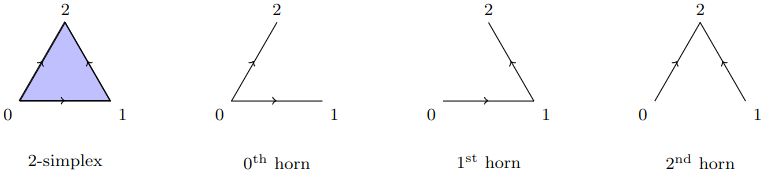
\includegraphics[width=1\textwidth]{simplicies.png}\caption{Inner horns on the 2-simplex}
    \end{figure}
\begin{remark}
    To any $\infty$-category there exists a homotopy category $\Ho(\cat C)$. 
    This has the same objects as $\cat C$ and whose morphisms correspond to homotopy classes of maps, where $f,g \colon x \to y$ are homotopic if there is a 2-simplex $\sigma \colon \Delta[2] \to \cat C$ with boundary $\partial \sigma  = (g,f,\text{id}_X)$, i.e, the boundary looks like
    % https://q.uiver.app/#q=WzAsMyxbMCwxLCJ4Il0sWzEsMCwieCJdLFsxLDEsInkiXSxbMCwxLCJcXHRleHR7aWR9X1giXSxbMCwyLCJmIiwyXSxbMSwyLCJnIl1d
\[\begin{tikzcd}[ampersand replacement=\&]
	\& x \\
	x \& y
	\arrow["{\text{id}_X}", from=2-1, to=1-2]
	\arrow["f"', from=2-1, to=2-2]
	\arrow["g", from=1-2, to=2-2]
\end{tikzcd}\]
\end{remark}
\begin{remark}
    If the lifting condition is satisfied for $0 \le k \le n$ we call it a Kan complex. For example, the singular complex of any topological space is a Kan complex.  
\end{remark}
If this seems a little abstract, consider the following example:
\begin{example}
    Any $1$-category $\cat C$ gives rise to an $\infty$-category via the nerve construction: We define a simplicial set $N(\cat C)$  with a 0-simplex for each object of $\cat C$, a 1-simplex for each morphism $f \colon x \to y$ in $\cat C$, a 2-simplex for each composition of morphisms and so on. We can also define face and degeneracy maps, either by inserting identity morphisms or `deleting' objects. The association $\cat C \to N(\cat C)$ defines a functor from the category of categories to simplicial sets. Moreover, one can show that that $N(\cat C)$ is an $\infty$-category: in fact, it is a special type called 2-coskeletal: morally, the simplicial set is generated by the data in dimensions 0, 1, and 2. 
\end{example}
\begin{figure}    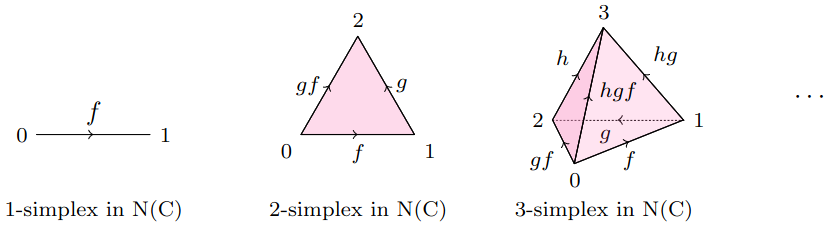
\includegraphics[width=1\textwidth]{simplicies2.png}\caption{The nerve of a category}
    \end{figure}
We are interested in a certain class of $\infty$-categories called stable. 
\begin{definition}
    An $\infty$-category $\cat C$ is called \emph{stable} if
    \begin{enumerate}
        \item $\cat C$ is \emph{pointed} i.e., it admits an object $0$ which is both initial and final;
        \item Every morphism $f \colon X \to Y$ in $\cat C$ admits a fiber $\fib(f)$ and a cofiber $\cofib(f)$, i.e., the following pullback and pushout squares exist:
        % https://q.uiver.app/#q=WzAsOCxbMCwwLCJcXGZpYihmKSJdLFsxLDAsIlgiXSxbMSwxLCJZIl0sWzAsMSwiMCJdLFsyLDAsIlgiXSxbMywwLCJZIl0sWzIsMSwiMCJdLFszLDEsIlxcY29maWIoZikiXSxbMCwxXSxbMSwyLCJmIl0sWzMsMl0sWzAsM10sWzAsMiwiIiwxLHsic3R5bGUiOnsibmFtZSI6ImNvcm5lci1pbnZlcnNlIn19XSxbNCw1LCJmIl0sWzQsNl0sWzYsN10sWzUsN10sWzcsNCwiIiwxLHsic3R5bGUiOnsibmFtZSI6ImNvcm5lci1pbnZlcnNlIn19XV0=
\[\begin{tikzcd}[ampersand replacement=\&]
	{\fib(f)} \& X \& X \& Y \\
	0 \& Y \& 0 \& {\cofib(f)}
	\arrow[from=1-1, to=1-2]
	\arrow["f", from=1-2, to=2-2]
	\arrow[from=2-1, to=2-2]
	\arrow[from=1-1, to=2-1]
	\arrow["\ulcorner"{anchor=center, pos=0.125}, draw=none, from=1-1, to=2-2]
	\arrow["f", from=1-3, to=1-4]
	\arrow[from=1-3, to=2-3]
	\arrow[from=2-3, to=2-4]
	\arrow[from=1-4, to=2-4]
	\arrow["\ulcorner"{anchor=center, pos=0.125, rotate=180}, draw=none, from=2-4, to=1-3]
\end{tikzcd}\]
\item A square in $\cat C$ of shape depicted below is a pullback if and only if it is a pushout:
% https://q.uiver.app/#q=WzAsNCxbMCwwLCJYIl0sWzEsMCwiWSJdLFsxLDEsIloiXSxbMCwxLCIwIl0sWzAsMV0sWzEsMl0sWzAsM10sWzMsMl1d
\[\begin{tikzcd}[ampersand replacement=\&]
	X \& Y \\
	0 \& Z
	\arrow[from=1-1, to=1-2]
	\arrow[from=1-2, to=2-2]
	\arrow[from=1-1, to=2-1]
	\arrow[from=2-1, to=2-2]
\end{tikzcd}\]
    \end{enumerate}
\end{definition}
This turns out to be equivalent to the following stronger looking condition. 
\begin{proposition}
    An $\infty$-category $\cat c$ is stable if and only if it has a zero object, admits finite
limits and colimits, and a general square in $\cat C$ is a pullback if and only if it is a pushout.
\end{proposition}
\begin{definition}
    Given an object in a stable $\infty$-category $\cat C$, we will write 
    \[
    \Sigma X \coloneqq \cofib(X \to 0) \quad \text{ and } \Omega X \coloneqq \fib(0 \to X)
    \]
\end{definition}
\begin{remark}
    One attractive feature of the theory of stable $\infty$-categories is that stability is a property of
$\infty$-categories, rather than additional data. The situation for additive categories is similar. Although additive
categories are often presented as categories equipped with additional structure (an abelian group structure
on all Hom-sets), this additional structure is in fact determined by the underlying category.
\end{remark}
\begin{remark}
    Let $f \colon A \to B$ be a morphism in $\cat C$, which we can then extend to a cofiber sequence:
    \[\begin{tikzcd}[ampersand replacement=\&]
	A \& B \\
	0 \& C
	\arrow[from=1-1, to=1-2]
	\arrow["p", from=1-2, to=2-2]
	\arrow[from=1-1, to=2-1]
	\arrow[from=2-1, to=2-2]
\end{tikzcd}\]
Since $\cat C$ is stable, $p$ admits a cofiber as well, so we can extend the square 
% https://q.uiver.app/#q=WzAsNyxbMCwwLCJBIl0sWzEsMCwiQiJdLFsxLDEsIkMiXSxbMCwxLCIwIl0sWzIsMCwiMCJdLFsyLDEsIkEnIl0sWzMsMSwiXFxTaWdtYSBBIl0sWzAsM10sWzAsMV0sWzEsMiwicCJdLFszLDJdLFsxLDRdLFsyLDUsInEiLDJdLFs0LDVdLFs1LDYsIiIsMSx7ImxldmVsIjoyLCJzdHlsZSI6eyJoZWFkIjp7Im5hbWUiOiJub25lIn19fV1d
\[\begin{tikzcd}[ampersand replacement=\&]
	A \& B \& 0 \\
	0 \& C \& {A'} \& {\Sigma A}
	\arrow[from=1-1, to=2-1]
	\arrow[from=1-1, to=1-2]
	\arrow["p", from=1-2, to=2-2]
	\arrow[from=2-1, to=2-2]
	\arrow[from=1-2, to=1-3]
	\arrow["q"', from=2-2, to=2-3]
	\arrow[from=1-3, to=2-3]
	\arrow[Rightarrow, no head, from=2-3, to=2-4]
\end{tikzcd}\]
with both squares pushouts. Since the outer square is a pushout as well, we can identify $A'$ with $\Sigma A$. Continuing in this fashion, we obtain
% https://q.uiver.app/#q=WzAsMTAsWzAsMCwiQSJdLFsxLDAsIkIiXSxbMSwxLCJDIl0sWzAsMSwiMCJdLFsyLDAsIjAiXSxbMiwxLCJcXFNpZ21hIEEiXSxbMSwyLCIwIl0sWzIsMiwiXFxTaWdtYSBCIl0sWzMsMSwiMCJdLFszLDIsIlxcU2lnbWEgQyJdLFswLDNdLFswLDFdLFsxLDIsInAiXSxbMywyXSxbMSw0XSxbMiw1LCJxIiwyXSxbNCw1XSxbMiw2XSxbNSw3XSxbNiw3XSxbNSw4XSxbNyw5XSxbOCw5XV0=
\[\begin{tikzcd}[ampersand replacement=\&]
	A \& B \& 0 \\
	0 \& C \& {\Sigma A} \& 0 \\
	\& 0 \& {\Sigma B} \& {\Sigma C}
	\arrow[from=1-1, to=2-1]
	\arrow[from=1-1, to=1-2]
	\arrow["p", from=1-2, to=2-2]
	\arrow[from=2-1, to=2-2]
	\arrow[from=1-2, to=1-3]
	\arrow["q"', from=2-2, to=2-3]
	\arrow[from=1-3, to=2-3]
	\arrow[from=2-2, to=3-2]
	\arrow[from=2-3, to=3-3]
	\arrow[from=3-2, to=3-3]
	\arrow[from=2-3, to=2-4]
	\arrow[from=3-3, to=3-4]
	\arrow[from=2-4, to=3-4]
\end{tikzcd}\]
and so we obtain a sequence
\[
A \to B \to C \to \Sigma A \to \Sigma B \to \Sigma C
\]
in which each consecutive pairs of maps admits a cofiber structure. This can be prolonged in either direction. 
\end{remark}
\begin{proposition}
    Let $\cat C$ be a stable $\infty$-category. Then $\Ho(\cat C)$ has a natural structure
of a triangulated category, where the shift functor is given by $\Sigma$ and the
distinguished triangles are given by the sequences $A \to B \to C \to \Sigma A$. 
described above.
\end{proposition}
\begin{example}
        Let $R$ be a commutative ring. Then there is an $\infty$-category
        \[
        \cat D(R) \coloneqq N(Ch(R))[q-iso^{-1}]
        \]
        obtained from the ordinary category of chain complexes by formally inverting the
quasi-isomorphisms between chain complexes. This $\infty$-category is stable and the
shift $[n]$ is given by shifting the chain complex by $n$.
\end{example}
\begin{definition}\label{def:stabilization}
Let $\cat C$ be a pointed $\infty$-category which admits finite limits and colimits (i.e., products, coproducts, and fibers and cofibers). In particular, we have a loopspace functor $\Omega \colon \cat C \to \cat C$.

We define the stabilization $\Sp(\cat C)$ to be the homotopy limit of the following diagram in $\mathrm{sSet}$:
\begin{center}
\begin{tikzcd}
\cdots \arrow[r]& \cat C \arrow["\Omega",r] & \cat C \arrow["\Omega",r] & \cat C.
\end{tikzcd}
\end{center}
$\Sp(\cat C)$ is a simplicial set with the following properties:
\begin{itemize}
\item $\Sp(\cat C)$ is a stable $\infty$-category.
\item There is an adjunction $\Sigma^\infty \colon \cat C \leftrightarrows \Sp(\cat C) \colon \Omega^\infty$.
\end{itemize}
\end{definition}
\begin{definition}
    The $\infty$-category of spectra $\Sp$ is the stabilization of the $\infty$-category of pointed topological spaces. 
\end{definition}
\begin{remark}
    The definition of stabilization is a proposition, rather than a definition, in \emph{Higher Algebra}. Lurie takes a different approach, and defines the stabilization as the category of functors $F \colon \mathcal{S}_*^{fin} \to \cat C$ from finite pointed spaces to $\cat C$ that are \emph{reduced} ($F$ preserves terminal objects) and \emph{excisive} ($F$ takes pushouts to pullbacks). He then shows that this is equivalent to the construction above. 
\end{remark}
The category of spectra has the following universal property:
\begin{theorem}
    Let $\cat D$ be a (presentable) stable $\infty$-category. Let $\LFun(\Sp, \cat D)$ denote the $\infty$-category of functors from $\Sp$ to $\cat D$ which have a right adjoint (equivalently, preserve colimits). Then, evaluation on the sphere spectrum $\mathbb S \coloneqq \Sigma^{\infty}(S^0)$ induces an equivalence of categories: $\LFun(\Sp, \cat D) \to \cat D$.
\end{theorem}
\begin{remark}
   This gives on way to product a smash product on the category of spectra: namely, as the composition:
   \[
   \Sp \times \Sp \simeq \LFun(\Sp,\Sp) \times \LFun(\Sp,\Sp) \xrightarrow{\circ} \LFun(\Sp,\Sp) \simeq \Sp
   \]   
   This is not the most useful definition, but it turns out to work. 
\end{remark}
\begin{remark}
  Let $\Pr^L_*$ denote the $\infty$-category of pointed presentable $\infty$-categories and left
functors between them (i.e. functors which admit right adjoints). Then one can show that the limit in \Cref{def:stabilization} is equivalent to the colimit in $\Pr^L_*$:
\[
\Sp(\cat C) \simeq \varinjlim(\cat C \xrightarrow{\Sigma} \cat C \xrightarrow{\Sigma} \cdots )
\]
\end{remark}

\section{$G$-spaces and $G$-spectra - first attempt}
We have seen that we have $G$-spaces, and so we can try and stabilize and talk about $G$-spectra. Our first guess might be to directly take the definition of spectra and put a $G$-everywhere. 
\begin{definition}
    A $G$-equivariant $S^1$ spectrum $E$ is a sequence of $G$-spaces $E = \{ E_n \}$  and equivariant maps $\sigma_n \colon \Sigma E_n \to E_{n+1}$.
    \end{definition}
This defines for us the so-called category of `naive' $G$-spectra. By a variant of Elmendorf's theorem, we have the following:
\begin{theorem}
    The category of naive $G$-spectra is equivalent to the category $\Fun(\mathcal{O}_G^{op},\Sp)$. 
\end{theorem}
Although these are not ultimately not what we will be interested in, they are still strong enough to represent $\mathbb{Z}$-graded cohomology theories. 
\begin{theorem}
    Every cohomology (resp.~homology) theory on $G$-CW complexes is represented (resp.~corepresented) by a naive $G$-spectrum.
\end{theorem}
So what is the problem? One motivation comes from duality. Let us say a few words about this. 
\begin{definition}
    Let $(\mathcal{C},\otimes,\mathbf{1})$ be a symmetric monoidal category. An object $B \in \mathcal{C}$ is a strong dual of an object $A$ if there exist morphisms
    \[
    \epsilon \colon B \otimes A \to \mathbf{1} \quad \text{ and } \eta \colon  \mathbf{1} \to B \otimes A
    \]
    called evaluation and coevaluation, which make the following diagrams commute:
    % https://q.uiver.app/#q=WzAsMyxbMCwwLCJcXG1hdGhiZnsxfSBcXG90aW1lcyBBIFxcY29uZyBBIl0sWzIsMCwiQSBcXGNvbmcgQSBcXG90aW1lcyBcXG1hdGhiZnsxfSJdLFsxLDEsIkEgXFxvdGltZXMgQiBcXG90aW1lcyBBIl0sWzAsMSwiXFx0ZXh0e2lkfV9BIl0sWzAsMiwiXFxldGEgXFxvdGltZXMgXFx0ZXh0e2lkfV9BIiwyXSxbMiwxLCJcXHRleHR7aWR9X0EgXFxvdGltZXMgXFxlcHNpbG9uIiwyXV0=
\[\begin{tikzcd}
	{\mathbf{1} \otimes A \cong A} && {A \cong A \otimes \mathbf{1}} \\
	& {A \otimes B \otimes A}
	\arrow["{\text{id}_A}", from=1-1, to=1-3]
	\arrow["{\eta \otimes \text{id}_A}"', from=1-1, to=2-2]
	\arrow["{\text{id}_A \otimes \epsilon}"', from=2-2, to=1-3]
\end{tikzcd}\]
and 
% https://q.uiver.app/#q=WzAsMyxbMiwwLCJcXG1hdGhiZnsxfSBcXG90aW1lcyBCIFxcY29uZyBCIl0sWzEsMSwiQiBcXG90aW1lcyBBIFxcb3RpbWVzIEIiXSxbMCwwLCJCIFxcY29uZyBCIFxcb3RpbWVzIFxcbWF0aGJmezF9Il0sWzEsMCwiXFxlcHNpbG9uIFxcb3RpbWVzIFxcdGV4dHtpZH1fQiIsMl0sWzIsMCwiXFx0ZXh0e2lkfV9CIl0sWzIsMSwiXFx0ZXh0e2lkfV9CIFxcb3RpbWVzIFxcZXRhICIsMl1d
\[\begin{tikzcd}
	{B \cong B \otimes \mathbf{1}} && {\mathbf{1} \otimes B \cong B} \\
	& {B \otimes A \otimes B}
	\arrow["{\epsilon \otimes \text{id}_B}"', from=2-2, to=1-3]
	\arrow["{\text{id}_B}", from=1-1, to=1-3]
	\arrow["{\text{id}_B \otimes \eta }"', from=1-1, to=2-2]
\end{tikzcd}\]
\end{definition}
Here are some properties, which will be left as an exercise. 
\begin{lemma} Let $B$ be a strong dual of $A$. 
    \begin{enumerate}
        \item $B$ is a strong dual of $A$ if and only if $A$ is a strong dual of $B$. 
        \item If $B$ is a strong dual of $A$, then there is an adjunction $ - \otimes A \dashv - \otimes B$. Deduce that the strong dual of $A$, if it exists, is unique up to isomorphism (we typically denote it by $\mathbf{D}A$). 
        \item If $\mathcal{C}$ is closed with internal hom $F(-,-)$, then the strong dual of an object $A$, if it exists, is $F(A,\mathbf{1})$. 
    \end{enumerate}
\end{lemma}
We often just say that $A$ is strongly dualizable if there exists a strong dual for $A$. These objects have many nice properties, for example the following:
\begin{proposition}\label{prop:dualizable-property}
    When $X$ or $Z$ is strongly dualizable, the map
    \[
    F(X,Y) \otimes Z \to F(X,Y \otimes Z)
    \]
    given by the composite
    \[
    F(X,Y) \otimes Z \cong F(X,Y) \otimes F(\mathbf{1},Z) \to F(X,Y \otimes Z)
    \]
    is an equivalence. 
\end{proposition}
\begin{example}
    Let $R$ be a commutative ring, and take $\mathcal{C} = (\Mod_R,\otimes_R,R)$. We first note that the unit of a symmetric monoidal category is always dualizable: in particular, $R$ is dualizable as an $R$-module. Moreover, dualizable objects are closed under retracts and direct sums, and hence any finitely-generated projective module is dualizable (as a retract of $R^n$). 

    We can define the (weak) dual of any object to be $\Hom_R(-,R)$. Then, $\epsilon_M \colon \Hom_R(M,R) \otimes M \to R$ is the usual evaluation map $f \otimes m \mapsto f(m)$. The coevalution map sends $1 \in R$ to a finite sum $\sum_{i \in I} m_i \otimes f_i$. The triangle identities above then give
    \[
    \sum_{i \in I}m_if_i(p) = p, \quad  p \in M
    \]
    and
    \[
    \sum_{i \in I}r(m_i)f_i = r, \quad r \in \Hom_R(M,R). 
    \]
 Now consider the map that sends $\alpha \colon R^I \to M$ that sends $(r_i)_{i \in I}$ to $\sum_{i \in I}m_ir_i$, and the map $\beta \colon M \to R^I$ that sends $p \in M$ to $(f_i(p))_{i \in I}$. The triangle identities then imply that $M$ is finitely generated and a retract of $R^I$ ($\alpha\beta = \text{id}_{M}$), i.e., $M$ is a finitely generated projective module. In other words: $M$ is strongly dualizable in $\Mod_R$ if and only if it is finitely generated and projective. 

 This example extends to chain complexes: a chain complex $M \in \Ch(R)$ is dualizable if and only if $M_q$ is finitely generated for all $q$ and $M_q \ne 0$ for only finitely many $q$, and $M_q$ is projective for all $q$. 
\end{example}
What about the category of spectra? A non-trivial result is the following:
\begin{theorem}
    Finite CW-spectra and their wedge summands are dualizable in the stable homotopy category. 
\end{theorem}
From \Cref{prop:dualizable-property} (with $Y = \mathbb{S}$) we deduce the following:
\begin{proposition}\label{prop:dualizable-iso}
    Let $X$ be a dualizable spectrum, then for all spectra $E$ we have 
    \[
    \mathbf{D}X \otimes E \to F(X,E)
    \]
    is an equivalence, and hence there is an isomorphism
    \[
    E_*(\mathbf{D}X) \coloneqq \pi_*(\mathbf{D}X \wedge E) \xrightarrow{\cong} \pi_*F(X,E) \coloneqq E^*(X). 
    \]
\end{proposition}
\begin{definition}
    Let $S^q$ be a sphere of dimension $q$. Let $\eta \colon S^q \to X \wedge Y$ and $\epsilon \colon Y \wedge X \to S^q$, then we say that $X$ and $Y$ are $q$-dual if following diagrams commute up to homotopy: 
    % https://q.uiver.app/#q=WzAsMyxbMCwwLCJTXnEgXFx3ZWRnZSBBIl0sWzIsMCwiQSBcXHdlZGdlIFNecSJdLFsxLDEsIkEgXFx3ZWRnZSBCIFxcd2VkZ2UgQSJdLFswLDEsIlxcdGF1Il0sWzAsMiwiXFxldGEgXFx3ZWRnZSBcXHRleHR7aWR9X0EiLDJdLFsyLDEsIlxcdGV4dHtpZH1fQSBcXHdlZGdlIFxcZXBzaWxvbiIsMl1d
\[\begin{tikzcd}
	{S^q \wedge A} && {A \wedge S^q} \\
	& {A \wedge B \wedge A}
	\arrow["\tau", from=1-1, to=1-3]
	\arrow["{\eta \wedge \text{id}_A}"', from=1-1, to=2-2]
	\arrow["{\text{id}_A \wedge \epsilon}"', from=2-2, to=1-3]
\end{tikzcd}\]
and
% https://q.uiver.app/#q=WzAsMyxbMiwwLCJTXnEgXFx3ZWRnZSBCIl0sWzEsMSwiQiBcXHdlZGdlIEEgXFx3ZWRnZSBCIl0sWzAsMCwiQiBcXHdlZGdlIFNecSJdLFsxLDAsIlxcZXBzaWxvbiBcXG90aW1lcyBcXHRleHR7aWR9X0IiLDJdLFsyLDAsIigtMSlebiBcXHRhdSJdLFsyLDEsIlxcdGV4dHtpZH1fQiBcXHdlZGdlIFxcZXRhICIsMl1d
\[\begin{tikzcd}
	{B \wedge S^q} && {S^q \wedge B} \\
	& {B \wedge A \wedge B}
	\arrow["{\epsilon \otimes \text{id}_B}"', from=2-2, to=1-3]
	\arrow["{(-1)^n \tau}", from=1-1, to=1-3]
	\arrow["{\text{id}_B \wedge \eta }"', from=1-1, to=2-2]
\end{tikzcd}\]
Here $\tau$ denotes the interchange map. 
\end{definition}
\begin{remark}
    Let $X$ and $Y$ be $q$-dual spaces. Then, $\mathbf{D}(\Sigma^{\infty}X) \simeq \Sigma^{-q}\Sigma^{\infty}Y$. 
\end{remark}
\begin{definition}
    Let $\xi \colon V \to M$ be a vector bundle, then the Thom space of $\xi$ is defined to be $T\xi \coloneqq D(V)/S(V)$ where $D(V)$ and $S(V)$ are the unit disc and sphere bundles associated to $\xi$.\footnote{Let $\xi \colon V \to M$ be a vector bundle, and choose a metric on $V$; then, the disc bundle $D(V)$ is the subset of vectors with $\norm{x} \le 1$, and the sphere
bundle $S(V)$ is the subset of vectors with $\norm{x} = 1$. These are fiber bundles with fiber $D^n$ and $S^{n-1}$, respectively.}
\end{definition}
Finally, we can state the duality theorem we are interested in.
\begin{theorem}[Atiyah duality]
   Let $M$ be a compact smooth $n$-dimensional manifold without boundary embedded in $\mathbb{R}^q$, and let $T\nu$ be the Thom space of its normal bundle $\nu$. Then $M_+$ and $T{\nu}$ are $q$-dual.
\end{theorem}
\begin{remark}
    In other words, $\mathbf{D}(\Sigma^{\infty}M_+) \simeq \Sigma^{-q}\Sigma^{\infty}T\nu$. 
\end{remark}
Let us explain how this gives a version of Poincar\'e duality. We need one final definition and theorem. 
\begin{definition}
    Let $E$ and $\widetilde{E}$ be a generalized cohomology theory and the corresponding reduced theory respectively. For a bundle $\xi: V \to M$ and the associated Thom space $T \xi$, let $i_x: S^n_x \to T \xi$ be the canonical map where $S^n_x$ is the one-point compactification of the fiber $\xi^{-1}(x)$ for each $x \in M$. An $E$-orientation of $\xi$ is an element of degree $n$ in $\widetilde{E}^n(T \xi)$ such that $i_x^*(\mu) \in \widetilde{E}^n(S^n_x)$ is a generator.
\end{definition}

\begin{theorem}[Thom isomorphism ]
    Let $\xi: V \to M$ be an $n$-dimensional bundle with an $E$-orientation $\mu \in \widetilde{E}^n(T \xi)$, then $\Phi$ given by
\[
- \cup \mu \colon  E^*(M) \to \widetilde{E}^{n+*}(T \xi)
\]
is an isomorphism.
\end{theorem} 
We now prove Poincar\'e duality. 
\begin{theorem}[Poincar\'e Duality]
Let $M$ be an $E$-orientable $n$-dimensional manifold without boundary, then there is an isomorphism
\[
E^*(M) \xrightarrow{\cong} E_{n-*}(M).
\]
\end{theorem}

\begin{proof}
Let $M$ be embedded in $\mathbb{R}^q$. The Poincar\'e duality map is given by the
composite of the Thom isomorphism and the duality isomorphism induced by the
$q$-dual pair $(M_+, T\nu)$:
\[
E^*(M) \rightarrow \widetilde{E}^{q-n+*}(T\nu) \rightarrow E_{n-*}(M).
\]
Since the normal bundle $\nu$ of the embedding $M \rightarrow \mathbb{R}^q$ has dimension $q - n$, the first
map is indeed given by the Thom isomorphism. Since $(M^+, T\nu)$ is a $q$-dual pair,
$(\Sigma^\infty M^+, \Sigma^{-q}\Sigma^\infty T\nu)$ is a dual pair of spectra, so
\[
\widetilde{E}^{q-n+*}(T\nu) \cong \widetilde{E}^{-n+*}(\Sigma^{-q}\Sigma^\infty T\nu) \rightarrow \widetilde{E}_{n-*}(\Sigma^\infty M_+) \cong E_{n-*}(M)
\]
is an isomorphism by \Cref{prop:dualizable-iso}.
\end{proof}
\begin{remark}
   A key point in the proof is that any manifold embeds into $\mathbb{R}^n$. Suppose now that we work with $G$-manifolds (that is manifolds with a $G$-action by smooth maps). There is an equivariant version of Whitney's theorem, due to Mostow and Palais:
   \begin{theorem}
       Let $M$ be a compact $G$-manifold, then there is a $G$-equivariant embedding $M \hookrightarrow V$, where $V$ is some finite dimensional real representation of $G$. 
   \end{theorem}
   We can then try and repeat all the above arguments, and you will see that representations spheres naturally enter the picture. In other words, if we want an equivariant version of Poincar\'e duality, we are forced to space with representations spheres that $G$-manifolds embed in. Thus, unless we are interested in manifolds with trivial $G$-action, we need to smash with representation spheres! 
\end{remark}

\begin{remark}
    Now we note that $G/H$ is always a smooth manifold, and in particular, the suspension spectrum $\Sigma^{\infty}G/H_+$ is dualizable in the category of spectra. Let us write $\Sp_{G}^{n}$ for the category of naive $G$-spectra. One can show that
    \[
    F_{\Sp_G^n}(\Sigma^{\infty}G/H_+,\mathbf{1}) \simeq \mathbf{1},
    \]
    and in particular, $\Sigma^{\infty}G/H_+$ cannot be dualizable unless $H = G$. 
\end{remark}
\begin{remark}
    Here is one final reason that representations naturally appear: the equivariant version of the Freudenthal suspension theorem. To see this up, let $X$ be a based $G$-space and define
    \[
    \Sigma^VX \coloneqq S^V \wedge X \quad \text{ and } \quad \Omega^VX \coloneqq [S^V,X]
    \]
    These are adjoint, i.e., 
    \[
    [\Sigma^VX,Y] \simeq [X,\Omega^VY]
    \]
    and we can construct the following diagram
    % https://q.uiver.app/#q=WzAsMyxbMCwwLCJbWCxZXSJdLFsxLDAsIltcXFNpZ21hXlZYLFxcU2lnbWFeVlldIl0sWzEsMSwiW1gsXFxPbWVnYV5WXFxTaWdtYV5WWF0iXSxbMCwxLCJcXFNpZ21hXlYiXSxbMSwyLCJcXGNvbmciXSxbMCwyLCJcXGV0YV8qIiwyXV0=
\[\begin{tikzcd}[ampersand replacement=\&]
	{[X,Y]} \& {[\Sigma^VX,\Sigma^VY]} \\
	\& {[X,\Omega^V\Sigma^VX]}
	\arrow["{\Sigma^V}", from=1-1, to=1-2]
	\arrow["\cong", from=1-2, to=2-2]
	\arrow["{\eta_*}"', from=1-1, to=2-2]
\end{tikzcd}\]
where $\eta$ is the unit of the adjunction. Let $c(X)$ denote the connectivity of a space, where $c(X) = -1$ if $X$ is not path connected. Let $\nu$ be a
function from conjugacy classes of subgroups of $G$ to $\mathbb{N} \cup \{ \infty \}$.
\begin{theorem}[Freudenthal Suspension]
The map $\eta \colon Y \rightarrow \Omega^V \Sigma^V Y$ is a $\nu$-equivalence if $\nu$ satisfies the following two conditions:
\begin{enumerate}
  \item $\nu(H) \leq 2c(Y^H) + 1$ for all subgroups $H$ with $\dim V^H > 0$.
  \item $\nu(H) \leq c(Y^K)$ for all pairs of subgroups $K \subset H$ with $\dim V^K > \dim V^H$.
\end{enumerate}
Therefore,\footnote{via Whitehead's theorem} the suspension map
\[
\Sigma^V \colon [X,Y] \to [\Sigma^VX,\Sigma^VY]
\]
is surjective if $\dim(X^H ) \le \nu(H)$ for all $H$, and bijective if $\dim(X^H) \le \nu(H) -1$.
\end{theorem}
So once again, representations spheres appear quite naturally. 
\end{remark}
\section{The category of genuine $G$-spectra}
Last time we convinced ourselves that a good theory of $G$-spectra will involve  inverting \emph{all} representation spheres, and not just that associated with the trivial representation. Since any representation sits inside a direct sum of copies of the regular representation it will suffice to invert that. We can do this in the following way:
\begin{definition}
    The $\infty$-category of (genuine) $G$-spectra $\Sp_G$ is the limit of the diagram
    \[
    \Sp_G \coloneqq \lim \left( \cdots \to G\Top_* \xrightarrow{\Omega^{\rho}} G\Top_* \xrightarrow{\Omega^{\rho}} G\Top_* \right)
    \]
\end{definition}

\begin{remark}
This type of construction has been studied by Robalo. Namely, given an $\infty$-category $\cat C$ and a functor $G \colon \cat C \to \cat C$ a functor with right adjoint $U$, one can define the stabilization as the limit
\[
\Stab_{(G,U)}(\cat C) \simeq \varprojlim \left( \cdots \to \cat C \xrightarrow{U} \cat C \xrightarrow{U} \cat C \right)
\]
If $\cat C$ is presentable, this is the colimit in $\Pr_L$ of 
\[
 \varinjlim \left( \cdots \to \cat C \xrightarrow{G}\cat C \xrightarrow{G} \cat C \right)
\]
\end{remark}
\begin{remark}
    There is an adjoint pair
    \[
    \Sigma^{\infty}_G \colon G\Top_* \leftrightarrows \Sp_G \colon \Omega^{\infty}_G
    \]
    It has also been checked that the definition of $G$-spectra agrees with the underlying $\infty$-category of the model category of orthogonal $G$-spectra. Finally, this also implies that every object can be written as 
    \begin{equation}\label{eq:g-presentation}
 X \simeq \varinjlim \mathbb{S}^{-n\rho} \wedge \Sigma_G^{\infty}\Omega_G^{\infty}(\mathbb{S}^{n\rho} \wedge X).
    \end{equation}
    \end{remark}
One advantage of (genuine) $G$-spectra is that they naturally represent $RO(G)$-graded cohomology theories. 
\begin{proposition}
   Let $V$ be a $G$-representation and $X$ a pointed $G$-CW complex. For any $G$-spectrum $E$, the assignment
    \[
    (V,X) \mapsto [\Sigma^{\infty}X,S^V \wedge E]_G
    \]
    together with the natural suspension isomorphism
    \[
    [\Sigma^{\infty}X,S^V \wedge E]_G \xrightarrow{\cong}  [\Sigma^{\infty}\Sigma^{W}X,S^{V \oplus W} \wedge E]_G 
    \]
    given an $RO(G)$-graded cohomology theory. 

    Conversely, if $E^*(-)$ represents an $RO(G)$-graded cohomology theory, then there is a $G$-specturm which represents it in the homotopy category. 
\end{proposition}
\begin{example}
    As discussed previously, suppose that $\ul{M}$ is a coefficient system which arises as the restriction of a Mackey functor, then Bredon cohomology $H_G^*(-,\ul{M})$ extends to an $RO(G)$-graded cohomology theory. The associated $G$-spectrum is the Eilenberg--MacLane spectrum $H\ul{M}$.
\end{example}
\begin{theorem}[Robalo, Gepner--Meier]\label{thm:robalo}
    Let $G$ be a finite group and let $\rho_G$ denote the regular representation of $G$. Given a presentably symmetric monoidal
$\infty$-category $\cat D$ and a symmetric monoidal left adjoint $ F \colon G\Top_* \to \cat D$ with the property
that $F(S^{\rho_G})$ is invertible, there exists an essentially unique symmetric monoidal left
adjoint $\overline F \colon \Sp_G \to \cat D$ such that $\overline{F} \circ \Sigma^{\infty}_G \simeq F$ as symmetric monoidal functors:
% https://q.uiver.app/#q=WzAsMyxbMCwwLCJHXFxUb3BfKiJdLFsxLDEsIlxcY2F0IEQiXSxbMCwxLCJcXFNwIl0sWzAsMSwiRiJdLFswLDIsIlxcU2lnbWFee1xcaW5mdHl9X0ciLDJdLFsyLDEsIlxcb3ZlcmxpbmV7Rn0iLDIseyJzdHlsZSI6eyJib2R5Ijp7Im5hbWUiOiJkYXNoZWQifX19XV0=
\[\begin{tikzcd}[ampersand replacement=\&]
	{G\Top_*} \\
	\Sp \& {\cat D}
	\arrow["F", from=1-1, to=2-2]
	\arrow["{\Sigma^{\infty}_G}"', from=1-1, to=2-1]
	\arrow["{\overline{F}}"', dashed, from=2-1, to=2-2]
\end{tikzcd}\]
\end{theorem}
\begin{proposition}
    Let $i \colon G \to G'$ be a morphism of groups. Then there is a symmetric monoidal left adjoint functor $i^* \colon \Sp_{G'} \to \Sp_G$. 
\end{proposition}
Since any group homomorphism $G \to G'$ factors as
\[
G \twoheadrightarrow G/\ker(i) \hookrightarrow G'
\]
 it suffices to treat the case of quotienting by a normal subgroup, and inclusions separately. 
  \begin{proposition}
     Let $G$ be a group and $H$ a subgroup, then there is a symmetric monoidal left adjoint functor
     \[
     \Res^G_H \colon \Sp_{G} \to \Sp_H
     \]
 \end{proposition}
 \begin{proof}
     We first prove that this exists on the level of spaces. We will use Elmendorf's theorem to identify
     \[
     G\Top_* \simeq \Fun(\mathcal{O}_{G}^{op},\Top_*)
     \]
     and similar for $H\Top_*$. We note that under this equivalence the regular representation sphere $S^{\rho_G}$ corresponds to the functor that assigns to $G/K$ the sphere $S^{|G/K|}$. 
     
     The functor $\Res^G_H \colon G\Top_* \to H\Top_*$ corresponds to the functor induced by $G \times_H - \colon \mathcal{O}_H \to \mathcal{O}_G$. 
        We now want to apply \Cref{thm:robalo} to the diagram:
% https://q.uiver.app/#q=WzAsNCxbMCwwLCJHXFxUb3BfKiJdLFsxLDEsIlxcU3BfSCJdLFswLDEsIlxcU3BfRyJdLFsxLDAsIkhcXFRvcF8qIl0sWzAsMiwiXFxTaWdtYV57XFxpbmZ0eX1fe0h9IiwyXSxbMiwxLCJcXFJlc15HX0giLDIseyJzdHlsZSI6eyJib2R5Ijp7Im5hbWUiOiJkYXNoZWQifX19XSxbMCwzLCJcXFJlc15HX0giXSxbMywxLCJcXFNpZ21hXntcXGluZnR5fV9HIl1d
\[\begin{tikzcd}[ampersand replacement=\&]
	{G\Top_*} \& {H\Top_*} \\
	{\Sp_G} \& {\Sp_H}
	\arrow["{\Sigma^{\infty}_{G}}"', from=1-1, to=2-1]
	\arrow["{\Res^G_H}"', dashed, from=2-1, to=2-2]
	\arrow["{\Res^G_H}", from=1-1, to=1-2]
	\arrow["{\Sigma^{\infty}_H}", from=1-2, to=2-2]
\end{tikzcd}\]
where we are taking $F$ as the composite $\Sigma_H^{\infty} \circ \Res_{H}^G$. Since $\Sigma^{\infty}_H$ inverts $S^{\rho_H}$ by construction, it suffices to show that $\Res^G_H \colon G\Top_* \to H\Top_*$ carries $S^{\rho_{G}}$ to an invertible object in $\Sp_H$. But in fact it carries $S^{\rho_G}$ to $S^{\Res^{G}_{H}{\rho_G}}$, which is invertible (as it is a representation sphere). 
 \end{proof}
 \begin{remark}
     The right adjoint to restriction is called coinduction. Perhaps surprisingly, coinduction is also \emph{left} adjoint to restriction, where it goes by the name induction. This theorem is called the Wirthm{\"u}ller isomorphism. 
 \end{remark}
 \begin{example}
     We have that 
     \[
     \Coind_H^G(\mathbb{S}_H) \simeq \Ind_H^G(\mathbb{S}_H) \simeq \Sigma^{\infty}_G G/H_+
     \]
     Indeed, one can show that there is a commutative diagram
     % https://q.uiver.app/#q=WzAsNCxbMCwwLCJIXFxUb3BfKiJdLFsxLDEsIlxcU3BfRyJdLFswLDEsIlxcU3BfSCJdLFsxLDAsIkdcXFRvcF8qIl0sWzAsMiwiXFxTaWdtYV57XFxpbmZ0eX1fe0h9IiwyXSxbMiwxLCJcXEluZF5HX0giLDJdLFswLDMsIlxcSW5kXkdfSCJdLFszLDEsIlxcU2lnbWFee1xcaW5mdHl9X0ciXV0=
\[\begin{tikzcd}[ampersand replacement=\&]
	{H\Top_*} \& {G\Top_*} \\
	{\Sp_H} \& {\Sp_G}
	\arrow["{\Sigma^{\infty}_{H}}"', from=1-1, to=2-1]
	\arrow["{\Ind^G_H}"', from=2-1, to=2-2]
	\arrow["{\Ind^G_H}", from=1-1, to=1-2]
	\arrow["{\Sigma^{\infty}_G}", from=1-2, to=2-2]
\end{tikzcd}\]
to reduce the a computation in $H$-spaces, where it is straightforward. 
 \end{example}
 \begin{proposition}
     Let $G$ be a group and $N$ a normal subgroup, then there is a symmetric-monoidal left adjoint functor
     \[
     \Inf_{G/N}^G \colon \Sp_{G/N} \to \Sp_G
     \]

 \end{proposition}
 \begin{proof}
Once again, this boils down to a statement about spaces, namely that there is a functor $(G/N)\Top_* \to G\Top_*$, namely the functor that takes a $G/N$-space and considers it as a $G$-space via the quotient map. 
\end{proof}
 \begin{remark}
     The right adjoint is known as the fixed points functor $(-)^N \colon \Sp_{G} \to \Sp_{G/N}$
 \end{remark}
 \begin{definition}
   For an arbitrary subgroup $H \le G$ the $H$-fixed point functor is the composite
   \[
   \Sp_G \xrightarrow{\Res^G_H} \Sp_H \xrightarrow{(-)^H} \Sp
   \]
 \end{definition}
 \begin{proposition}
     The fixed point functor $(-)^H$ is corepresented by $\Sigma_G^{\infty}G/H_+$. \textbf{}
 \end{proposition}
 \begin{proof}
     This is more or less formal from what we have so far: for $M \in \Sp_G$ we have
     \[
     \begin{split}
     M^H \simeq \Hom_{\Sp}(\mathbb{S},M^H) & \simeq \Hom_{\Sp}(\mathbb{S},(\Res^G_HM)^H) \\ & \simeq \Hom_{\Sp_H}(\Inf_{e}^H\mathbb{S},\Res^G_HM) \\& \simeq \Hom_{\Sp_H}(\mathbb{S}_H,\Res^G_HM) \\
     & \simeq \Hom_{\Sp_G}(\Coind_H^G \mathbb{S}_H,M) \\
     & \simeq \Hom_{\Sp_G}(\Sigma^{\infty}_GG/H_+,M) \qedhere
     \end{split}
     \]
 \end{proof}
 \begin{remark}
     The category $\Sp_G$ is closed: there is an internal hom $G$-spectrum $F(X,Y)$. The fixed points of this are computed by
     \[
     F(X,Y)^G \simeq \Hom_{\Sp_G}(\Sigma^{\infty}G/G_+,F(X,Y)) \simeq \Hom_{\Sp_G}(X,Y)
     \]
     In particular,
     \[
     F(\Sigma^{\infty}G/H_+,Y)^G \simeq Y^H. 
     \]
 \end{remark}
  \begin{definition}
     For $H \le G$ and $G$-spectrum $M$ we define
     \[
     \pi_n^H(M) \coloneqq \pi_n(M^H).
     \]
 \end{definition}
 \begin{remark}
     We would like our theory to have $\pi_*^H(M) = 0$ if and only if $M = 0$. Indeed, if we used the theory of model categories, this would have held essentially by definition. By the above, this is the same as saying that 
     \[
     M \simeq 0 \iff \pi_*\Hom_{\Sp_G}(\Sigma^{\infty}_GG/H_+,M) \simeq 0 \text{ for all } H \le G
     \]
     By general machinery, this is the same as saying that the smallest \emph{localizing subcategory} (a stable subcategory that is closed under retracts, extensions and colimits) containing $\Sigma_G^{\infty}G/H_+$ is all of $\Sp_G$. Here is a proof from our perspective. 
 \end{remark}
 \begin{proposition}
     The smallest localizing subcategory of $\Sp_G$ containing $\{\Sigma_G^{\infty}G/H_+\}_{H \le G}$ is $\Sp_G$. 
 \end{proposition}
 \begin{proof}
    Let $\cat C$ denote the localizing subcategory in question.  The analogous statement is true for pointed spaces, and since $\Sigma^{\infty}$ a left adjoint, all suspension spectra are in $\cat C$. We claim that if $X,Y \in \cat C$, then so is $X \wedge Y$. Indeed, one can reduce this to show that $\Sigma^{\infty}_G G/H_+ \wedge \Sigma^{\infty}_H G/K_+$ is in $\cat C$. But this follows from the double coset formula:
    \[
    \Sigma^{\infty}_G G/H_+ \wedge \Sigma^{\infty}_G G/K_+ \simeq \bigvee_{[g] \in H\backslash G/H} \Sigma^{\infty}_G G/(H^g \cap K)_+
    \]
    Moreover, orbits are self-dual, and so $\mathbb{D}(\Sigma^{\infty}_GX)$ is also in $\cat C$, for all finite pointed $G$-CW complexes $X$. In particular, $\mathbb{S}^{-n\rho} \in \cat C$. But then, the result follows from \eqref{eq:g-presentation}:
    \[
 X \simeq \varinjlim \mathbb{S}^{-n\rho} \wedge \Sigma_G^{\infty}\Omega_G^{\infty}(\mathbb{S}^{n\rho} \wedge X).\qedhere
    \]
 \end{proof}
 \begin{theorem}
     The groups $\{\pi_n^H(X)\}_{H \le G}$ assemble into a Mackey functor, denoted $\underline{\pi}_n(X)$. 
 \end{theorem}
 \begin{proof}
     We must construct the relevant transfer, restriction, and conjugation maps. The key observation is that by the Wirthm{\"u}ller isomorphis we have equivalences
     \[
[S^n,\Sigma^{\infty}G/H_+ \wedge X]_G \cong [S^n,\Coind^G_H\Res^G_HX]_G \cong    [\Sigma^{\infty}G/H_+ \wedge S^n,X]_G
     \]
     We then can define
     \[
     \begin{split}
     \Res^H_K &\colon  [\Sigma^{\infty}G/H_+ \wedge S^n,X]_G \to  [\Sigma^{\infty}G/K_+ \wedge S^n,X]_G  \\
     \Tr^H_K &\colon  [ S^n,\Sigma^{\infty}G/K_+ \wedge X]_G \to  [ S^n,\Sigma^{\infty}G/H_+ \wedge X]_G  \\
     \end{split}
     \]
     to be the maps induced by $G/K \to G/H$, while the conjugation map
     \[
     c_g \colon [\Sigma^{\infty}G/H_+ \wedge S^n,X]_G \to [\Sigma^{\infty}G/gHg^{-1}_+ \wedge S^n,X]_G
     \]
     is the obvious map induced by conjugation.  The verification that this form a Mackey functor almost follows because everything is done at the level of $G$-sets - the hardest thing to show is the double coset formula.
 \end{proof}
 \begin{remark}
     This is a nice feature of genuine stable equivariant homotopy that is not true on the level of spaces, or for naive $G$-spectra. We will give an example on the exercise sheet next week. 
 \end{remark}
 \begin{example}
     Let $\ul{M}$ be a Mackey functor, then the Eilenberg--MacLane spectrum $H\ul{M}$ mentioned previously is characterized by the property that
     \[
     \underline{\pi}_i(H\ul{M}) \cong \begin{cases}\ul{M} & i = 0 \\ 0 & \text{else.} \end{cases}
     \]
 \end{example}
 \chapter{Fixed point functors}
 \section{Isotropy separation and geometric fixed points}
 One of the main techniques for proving statements about $G$-spectra is via the method of isotropy separation, which we now explain. 
 \begin{definition}
     A \emph{family} $\mathcal F$ of subgroups of $G$ is a set of subgroups of $G$ which are closed under taking subgroups and conjugation. 
 \end{definition}
 \begin{example}
     Typically families include: the family of all subgroups, the family consisting of only the trivial subgroup, and the family of \emph{proper} subgroups. 
 \end{example}
 \begin{lemma}
     There exists a $G$-space $E\mathcal{F}$ determined up to equivalence by the conditions that
     \[
     E\mathcal{F}^K \simeq \begin{cases} \ast &\text{if } K \in \mathcal{F} \\
     \varnothing &\text{otherwise}.\end{cases}
     \]
 \end{lemma}
 \begin{proof}
     This is a consequence of Elmendorf's theorem, although a direct construction exists: if we let $i \colon \mathcal{O}_{\mathcal F}(G) \to \mathcal{S}_G$ denote the inclusion of the full subcategory of $G$-spaces spanned by the transitive $G$-sets with isotropy in $\mathcal{F}$, then 
     \[
     E\mathcal{F} \simeq \hocolim_{\mathcal{O}_{\mathcal{F}}}i.\qedhere
     \]
 \end{proof}
 The explicit construction shows that if $\mathcal{F}' \subseteq \mathcal{F}$ is a subfamily, then there is an induced map $E\mathcal{F}' \to E\mathcal{F}$. 
 \begin{example}
     If $\mathcal{F}$ is the family consisting of the trivial subgroup, then $E\mathcal{F} \simeq EG$ the universal cover of $BG$. If $\mathcal{F}$ is the family of all subgroups, then a point is model for $E\mathcal{F}$. If $\mathcal{F}$ is the family of proper subgroups, this is usually denoted by $E\mathcal{P}$. The does have an explicit model: it is
     \[
     E\mathcal{P} \simeq \hocolim_n S(n\overline{\rho}_G),
     \]
     where $\overline{\rho}_G$ is the reduced regular representation, the quotient of the regular representation by the trivial representation. 
 \end{example}
 \begin{definition}
     If $\mathcal{F}$ is a family, then let $E\mathcal{F}_+ \to S^0$
be the pointed map which sends $E\mathcal{F}$ to the non-basepoint. Let $E\mathcal{F}$ denote the cofiber.
 \end{definition}
 The next two results are left for the exercise sheet. 
 \begin{lemma}
     We have
     \[
     \tilde E\mathcal{F}^K \simeq \begin{cases} S^0 &\text{if } K \not \in \mathcal{F} \\
     \ast &\text{otherwise}.\end{cases}
     \]
 \end{lemma}
 \begin{lemma}
     Let $\mathcal{F}_1$ and $\mathcal{F}_2$ be families of subgroups of $G$. Then:
     \begin{enumerate}
         \item $\mathcal{F}_1 \cap \mathcal{F}_2$ is a family, and $E(\mathcal{F}_1 \cap \mathcal{F}_2) \simeq E\mathcal{F}_1 \times E\mathcal{F}_2$. 
         \item $\mathcal{F}_1 \cup \mathcal{F}_2$ is a family and $\tilde E(\mathcal{F}_1 \cup \mathcal{F}_2) \simeq \tilde E\mathcal{F}_1 \times \tilde E\mathcal{F}_2$. 
     \end{enumerate}
 \end{lemma}
 \begin{definition}
     For any pointed $G$-space $X$ and family $\mathcal{F}$ the isotropy separation sequence is the cofiber sequence of spaces
     $E\mathcal{F}_+ \to S^0 \to \tilde E\mathcal{F}$.
 \end{definition}
 The following follows directly by applying fixed points. 
 \begin{proposition}
     Let $X$ be a pointed $G$-space and $\mathcal{F}$ a family of subgroups of $G$. 
     \begin{enumerate}[label=(\alph*)]
         \item For any $H \in \mathcal{F}$, the map
         \[
         \Res^G_H(E\mathcal{F}_+ \wedge X) \to \Res^G_H(X)
         \]
         is an equivalence on $H$-fixed points and $\Res^G_H(\tilde E\mathcal{F} \wedge X)$ is contractible. 
         \item For any $K \not \in \mathcal{F}$, the map
         \[
         \Res^G_K (X) \to \Res^G_K(\tilde E\mathcal{F} \wedge X)
         \]
         is a $K$-equivalence and $\Res^G_K( E\mathcal{F}_+ \wedge X)$ is contractible. 
     \end{enumerate}
     In other words: We can break our $G$-space $X$ up into two conceptually simpler pieces:
     \begin{enumerate}[label=(\alph*)]
     \item A space $E\mathcal{F}_+ \wedge X$ whose isotropy is contained in $\mathcal{F}$.
     \item A space $\tilde E \mathcal{F} \wedge X$ which is contractible when restricted to any subgroup in $\mathcal{F}$. 
     \end{enumerate}
 \end{proposition}
 This leads to the important geometric fixed points functor.
 \begin{definition}
     Let $X \in \Sp_G$, then the  geometric fixed points functor $
     \Phi^G \colon \Sp_G \to \Sp$ is defined as
     \[
     \Phi^G(X) \coloneqq (\Sigma^{\infty} \tilde E\mathcal{P} \wedge X)^G
     \]
     where $\mathcal{P}$ is the family of proper subgroups of $G$. More generally, let $N$ be a normal subgroup, and let $\mathcal{F}[N] \coloneqq \SET{H \le G}{N \not \subseteq H}$, then we can define the partial geometric fixed points as the functor $\tilde \Phi^N \colon \Sp_G \to \Sp_{G/N}$
     \[
     \tilde\Phi^N(X) \coloneqq (\Sigma^{\infty} \tilde E\mathcal{F}[N] \wedge X)^N. 
     \]
 \end{definition}
 \begin{definition}
     For an arbitrary subgroup $H \le G$ we define $\Phi^H \colon \Sp_G \to \Sp$ to be the composite
     \[
     \Sp_G \xrightarrow{\Res^G_{H}} \Sp_{H} \xrightarrow{\Phi^H} \Sp
     \]
 \end{definition}
 \begin{remark}
     One can show that this is the same as the composite
     \[
     \Sp_G \xrightarrow{\Res^G_{N_GH}} \Sp_{N_GH} \xrightarrow{\tilde \Phi^H} \Sp_{W_GH} \xrightarrow{\Res^{W_GH}_e} \Sp
     \]
     We will later denote the composite of the first two maps as $(-)^{\phi H}$. 
 \end{remark}
 \begin{remark}
     Note that there is a natural map $X^G \to \Phi^G(X)$ coming from the map $S^0 \to \tilde E\mathcal{P}$. 
 \end{remark}
We can also construct $\tilde \Phi^N$ by the universal property. 
\begin{definition}
    Let $\tilde \Phi^N$ be the functor defined by the universal property
   % https://q.uiver.app/#q=WzAsNCxbMCwwLCJHXFxUb3BfKiJdLFsxLDAsIihHL04pXFxUb3BfKiJdLFswLDEsIlxcU3BfRyJdLFsxLDEsIlxcU3Bfe0cvTn0iXSxbMCwxLCIoLSleTiJdLFswLDIsIlxcU2lnbWFee1xcaW5mdHl9IiwyXSxbMiwzLCJcXHRpbGRlIFxcUGhpXk4iLDJdLFsxLDMsIlxcU2lnbWFee1xcaW5mdHl9Il1d
\[\begin{tikzcd}[ampersand replacement=\&]
	{G\Top_*} \& {(G/N)\Top_*} \\
	{\Sp_G} \& {\Sp_{G/N}}
	\arrow["{(-)^N}", from=1-1, to=1-2]
	\arrow["{\Sigma^{\infty}}"', from=1-1, to=2-1]
	\arrow["{\tilde \Phi^N}"', from=2-1, to=2-2]
	\arrow["{\Sigma^{\infty}}", from=1-2, to=2-2]
\end{tikzcd}\]
\end{definition}
Of course, it is not clear that these are the same functor, but one can check it is true (or take the second as the `correct' definition). 
\begin{remark}
    This implies that $\tilde \Phi^N$  has a right adjoint $\phi_N^* \colon \Sp_{G/N} \to \Sp_G$. This is sometimes called geometric inflation. We have
    \[
    \phi_N^* \simeq \Sigma^{\infty}\tilde E\mathcal{F}[N] \wedge \Inf_{G/N}^G(Y)
    \]
\end{remark}
\begin{lemma}
    We have $\tilde \Phi^N\Inf_{G/N}^G \simeq \textrm{id}$. 
\end{lemma}
\begin{proof}
    This follows by essential uniqueness and and the corresponding statement on spaces. 
\end{proof}
\begin{proposition}
    Geometric fixed points $\Phi^H \colon \Sp_G \to \Sp$ satisfy the following properties:
  \begin{enumerate}[label=(\alph*)]
    \item They are symmetric monoidal. 
    \item They preserve colimits. 
    \item If $X$ is a pointed $G$-space, then
    \[
    \Phi^H(\Sigma^{\infty}X) \simeq \Sigma^{\infty}(X^H).
    \]
\end{enumerate}
\begin{remark}\label{rem:weyl-group}
    Less obvious, but still true, is that $H$-geometric fixed points have a residual action by the Weyl group; that is, they refine to a functor
    \[
    \Phi^H \colon \Sp_G \to \Fun(BW_GH,\Sp).
    \]
\end{remark}
\end{proposition}
Geometric fixed points can also be used to detect weak equivalences. 
\begin{theorem}
Let $f \colon X \to Y$ be a morphism in $\Sp_G$, then the following are equivalent:
\begin{enumerate}[label=(\alph*)]
\item $f$ is an equivalence.
\item $f^H$ is an equivalence for all $H \le G$.
\item $\Phi^H(f)$ is an equivalence for all $H \le G$. 
\end{enumerate}
\end{theorem}
\begin{proof}
    We have already seen that $(a)$ and $(b)$ are equivalent. It is also clear that $(a)$ implies $(c)$. It therefore suffices to show that $(c)$ implies $(b)$. We proceed by induction on $G$, with the base case of $G = e$ being trivially true. By induction, we can assume that the claim is true for all proper subgroups of $G$. In particular, this means that 
    \[
    (\Res^G_HX)^H \to (\Res^G_HY)^H
    \]
    is an equivalence, or in other words
    \[
    f^H \colon X^H \to Y^H
    \]
    is an equivalence for all $H \lneq G$. This it remains to show that $f^G$ is an equivalence. Letting $Z$ be the cofiber of $f$ (so that $Z^H \simeq \ast$ for all $H \lneq G$), this is equivalent to showing that $Z^G$ is contractible. Now we use isotropy separation, in the form of the cofiber sequence
    \[
    (\Sigma^{\infty}E\mathcal{P}_+ \wedge Z)^G \to Z^G \to (\Sigma^{\infty}\tilde E\mathcal{P} \wedge Z)^G
    \]
    By the following lemma $Z^G \to (\Sigma^{\infty}\tilde E\mathcal{P} \wedge Z)^G$ is an equivalence, and so $Z^G \simeq \Phi^G(Z) \simeq \ast$, which completes the theorem. 
\end{proof}
\begin{lemma}
    Let $X$ be a $G$-spectrum, and $\mathcal{F}$ a family. Then $X \to \Sigma^{\infty}\tilde E\mathcal{F} \wedge X$ is an equivalence if and only if $X^H \simeq \ast$ for all $H \in \mathcal{F}$. 
\end{lemma}
\begin{proof}
    Suppose that $X \to \Sigma^{\infty}\tilde E\mathcal{F} \wedge X$ is an equivalence and $H \in \mathcal{F}$.  We note that
    \[
    \Res^G_H(\Sigma^{\infty}\tilde E\mathcal{F} \wedge X) \simeq \Sigma^{\infty}\Res^G_H(\tilde E\mathcal{F}) \wedge \Res^G_H(X)
    \]
    because restriction is symmetric monoidal and commutes with suspension.  Observe that if $K \le H$ (so that $K \in \mathcal{F}$) 
    \[
    (\Res^G_H(\tilde E\mathcal{F}))^K \simeq (\tilde E\mathcal{F})^K \simeq \ast.
    \]
    In other words, $\Res^G_H(\tilde E\mathcal{F})$ is contractible and so $X^H$ is as well. 

    Suppose then that $X^H \simeq \ast$ for all $H \in \mathcal{F}$. It suffices to show that $\Sigma^{\infty}E\mathcal{F}_+ \wedge X \simeq \ast$. By the construction of the classifying space it suffices to show that $\Sigma^{\infty}G/H_+ \wedge X$ for $H \in \mathcal{F}$. We can check this after fixed points where we have 
    \[
(\Sigma^{\infty}G/H_+ \wedge X)^K \simeq \Hom_{\Sp_G}(\Sigma^{\infty}(G/H_+ \wedge G/K_+),X) \simeq \bigvee_{G/H' \subseteq G/H \times G/K} X^{H'}
    \]
    But all these summands are zero, and the claim follows. See also  \cite[Proposition II.9.2]{LMS} for a slightly different proof. 
\end{proof}
\section{Tom--Dieck Splitting}

One can wonder if the fixed point functor for spaces and spectra commute: that is, do we have
\[
\Sigma^{\infty}(X^H) \simeq (\Sigma^{\infty}X)^H.
\]
However, we can easily see that this doesn't hold: we have
\[
(\Sigma^{\infty}G_+)^G \simeq (\Coind_e^G \mathbb{S})^G \simeq \Hom_{\Sp_G}(\Sigma^{\infty}G/G_+,\Coind_e^G\mathbb{S}) \simeq \mathbb{S}
\]
while
\[
\Sigma^{\infty}(G_+^G) \simeq \ast.
\]
This is part of a general result, known as tom-Dieck splitting. In fact, we will give an extension of tom-Dieck splitting, due to Lewis.
We will use a slightly different version of geometric fixed points:
\begin{definition}
    For a subgroup $H \le G$ let $X^{\phi H}$ be the image of $X$ under the composite
    \[
    \Sp_G \xrightarrow{\Res^G_{N_GH}} \Sp_{N_GH} \xrightarrow{\tilde \Phi^H} \Sp_{W_GH}
    \]
    We still have $(\Sigma^{\infty} X)^{\Phi H} \simeq \Sigma^{\infty} X^H$ if we interpret $(-)^H$ now as the composite
    \[
    \Sp_G \xrightarrow{\Res^G_{N_GH}} \Sp_{N_GH} \xrightarrow{(-)^H} \Sp_{W_GH}
    \]
\end{definition}
\begin{remark}
    The previous and new definitions are related: there is an equivalence $\Res^{W_GH}_{e}(X^{\phi H}) \simeq \Phi^H(X)$. 
\end{remark}
Our version of tom Dieck splitting will rely on the following definition:
\begin{definition}
    Let $X \in \Sp_G$, then a splitting of $X$ at $H$ is a map $f_H$ in $\Sp_{W_GH}$ 
% https://q.uiver.app/#q=WzAsMixbMCwwLCJYXkgiXSxbMSwwLCJYXntcXHBoaSBIfSJdLFswLDFdLFsxLDAsImZfSCIsMix7ImN1cnZlIjoxfV1d
\[\begin{tikzcd}[ampersand replacement=\&]
	{X^H} \& {X^{\phi H}}
	\arrow[from=1-1, to=1-2]
	\arrow["{f_H}"', curve={height=6pt}, from=1-2, to=1-1]
\end{tikzcd}\]
which splits the canonical map $X^H \to X^{\phi H}$. A $G$-splitting of $X$ is a choice of splitting at each subgroup $H \le G$. 
\end{definition}
\begin{example}
    Any $X \in \Sp_G$ is spit at $e$, since $X^e = X^{\phi e}$ by definition. 
\end{example}
\begin{lemma}
  Suspension spectra are split at any $H \le G$.  
\end{lemma}
\begin{proof}
We construct a map $\Sigma^{\infty}(Y^H) \to (\Sigma^{\infty} Y)^H$ that gives the splitting. Let $\pi \colon N_GH \to W_GH$ denote the quotient map, then the counit of the adjunction ($\Inf_{W_GH}^{N_GH},(-)^H)$ on based $N_GH$-spaces yields a map $\Inf_{N_GH}^{W_GH}(Y^H) \to Y$, and hence a map $\Inf_{N_GH}^{W_GH}(\Sigma^{\infty}(Y^H) \to \Sigma^{\infty}Y$ in spectra, whose adjoint is the desired map
\[
\Sigma^{\infty}(Y^H) \to (\Sigma^{\infty}Y)^H \qedhere
\]
\end{proof}
\begin{remark}
If $X$ and $Y$ are split at $H$, then so is $X \wedge Y$. Indeed, a splitting is given by the composite
\[
(X \wedge Y)^{\phi H} \cong X^{\phi H} \wedge Y^{\phi H} \xrightarrow{f_H \wedge g_H} X^H \wedge Y^H \to (X \wedge Y)^H.
\]
where the last morphism comes from lax monoidality of fixed points. 
\end{remark}

\begin{definition}
Let $X \in \Fun(BG,\Sp)$, then the homotopy orbits are $X_{hG} \coloneqq \colim_{BG}X$. For $X \in \Sp_G$, we define $X_{hG} = (\Res^G_eX)_{hG}$. 
\end{definition}
\begin{remark}
    One can show that there is a natural equivalence $X_{hG} \simeq (\Sigma^{\infty}EG_+ \wedge X)^G$. 
\end{remark}
\begin{remark}
    We will use the following result (the \emph{projection formula}): if $H \le G$, then $(\Ind_H^G,\Res_H^G)$ satisfies the projection formula:
    \[
    (\Ind_H^GY) \wedge X \simeq \Ind_H^G(Y \wedge \Res^G_HX)
    \]
    for $X \in \Sp_G$ and $Y \in \Sp_H$. Here the map is constructed as the adjoint of the composite
    \[
    \Res^G_H((\Coind_H^GY) \wedge X) \simeq   \Res^G_H(\Coind_H^GY) \wedge \Res^G_H(X) \to  Y \wedge \Res^G_H(X)
    \]
    Everything in sight preserves colimits, so it suffices to check it is an equivalence when $Y = \Sigma^{\infty}H/K$ and $X = \Sigma^{\infty}G/J$, where it is formal. 

    In fact, a more general statement is true: given an adjoint pair $(f^*,f_*)$, then the projection formula always holds for dualizable objects. 
    \end{remark}
    \begin{remark}\label{rem:commutative}
        There is a commutative diagram of groups: 
\[\begin{tikzcd}[ampersand replacement=\&]
	{N_GH} \& G \\
	{W_GH} \& e
	\arrow[hook, from=1-1, to=1-2]
	\arrow[two heads, from=1-2, to=2-2]
	\arrow[two heads, from=1-1, to=2-1]
	\arrow[two heads, from=2-1, to=2-2]
\end{tikzcd}\]
This implies that for any $X \in N_GH$
\[
(\Ind_{N_GH}^GX)^G \simeq (X^{H})^{W_GH}
\]
Indeed, both are right adjoint to inflation along $N_GH \to e$. 

Combining with the previous remark, we see that if $Y$ is a $G$-spectrum, then 
\[
((X \wedge \Res^{G}_{N_GH}Y)^H)^{W_GH} \simeq (\Ind_{N_GH}^G(X \wedge \Res^{G}_{N_GH}Y))^G \simeq (\Ind_{N_GH}^G(X) \wedge \Res^{G}_{N_GH}Y)^G
\]
    \end{remark}
    \begin{remark}
We construct the map used. We let $EW_GH_+$ denote the universal $W_GH$-space; by way of inflation along $N_GH \twoheadrightarrow W_GH$ we can also consider it as an $N_GH$ space. We omit writing this all the time. 

To that end, suppose that $X \in \Sp_G$ be $G$-split and consider the following composite\footnote{We think of $X$ occasionally of an $N_GH$ spectrum via restriction, and similarly, $\Sigma^{\infty}(EW_GH)_+$ as an $N_GH$ spectrum via inflation}
    \[
    \begin{split}
        (X^{\phi H})_{hW_GH} &\simeq \left(\Sigma^{\infty} (EW_GH)_+ \wedge X^{\phi H}\right)^{W_GH} \\
        & \simeq \left((\Sigma^{\infty}(EW_GH)_+ \wedge X)^{\phi H}\right)^{W_GH} \\
        &\xrightarrow{(f_H)_*}  \left((\Sigma^{\infty}(EW_GH)_+ \wedge X)^{H}\right)^{W_GH}  \\
        & \simeq \left(\Ind_{N_GH}^G\Sigma^{\infty}(EW_GH)_+ \wedge X\right)^{G} \\
        & \to X^G,
    \end{split}
    \]
    where the last map is induced by the map $(EW_GH)_+ \to S^0$. Call this map $\Theta_{X,H}$. Together, we define a map
    \[
    \Theta_X \colon \bigvee_{(H)}  (X^{\phi H})_{hW_GH} \to  X^G
    \]
    as the sum over the maps $\Theta_{X,H}$. 
\end{remark}
The theorem we want to prove is the following. 
\begin{theorem}\label{thm:tom-dieck-theorem}
    Let $X \in \Sp_G$ be a $G$-split $G$-spectrum, then the map 
    \[
 \Theta_X \colon \bigvee_{(H)} (X^{\phi H})_{hW_GH} \to  X^G
    \]
    is an equivalence of spectra. 
\end{theorem}
\begin{corollary}[Tom-Dieck splitting]
    Let $X \in G\Top_*$, then 
    \[
    (\Sigma^{\infty}X)^G \simeq \bigvee_{(H)} \Sigma^{\infty}(X^H)_{hW_GH}
    \]
\end{corollary}
\begin{remark}
    Note that the summand corresponding to $H = G$ is exactly $\Sigma^{\infty}(X^G)$. So this measures the failure of $G$-fixed points to commute with suspension spectra. 
\end{remark}
\begin{example}
    Take $X = G_+$ as before. Then all terms vanish except the contribution coming from $H = e$ where the summand contributes a copy of $\mathbb{S}$. 
\end{example}
\begin{example}
    Take $X = S^0 = G/G_+$, we see that
    \[
    \pi_0^G(\mathbb{S}^0_G) \cong \bigoplus_{(H)} \pi^{W_GH}_0(EW_GH_+) 
    \]
    One can show that each summand contributes a $\mathbb{Z}$, so that 
    \[
    \pi_0^G(\mathbb{S}^0_G)  \cong \mathbb{Z}\{ \text{conjugacy classes of subgroups}\}
    \]
    In fact, $\pi_0^G \cong A(G)$, the Burnside ring of finite $G$-sets. 
\end{example}
We now return to the proof of \Cref{thm:tom-dieck-theorem}. It relies on studying families a little more closely. 
\begin{definition}
    We say that two families $\mathcal{F}'\subseteq \mathcal{F}$ are \emph{adjacent} if there is a subgroup $H$ such that 
    \[
    \mathcal{F}\setminus \mathcal{F}' = \{ (H) \}.
    \]
\end{definition}
\begin{remark}\label{rem:filtration}
    There exists a filtration
    \[
    \varnothing = \mathcal{F}_{-1} \subseteq \mathcal{F}_0 \subseteq \ldots \subseteq \mathcal{F}_n = \mathcal{F}_{all}
    \]
    such that each pair $\mathcal{F}_i \subseteq \mathcal{F}_{i+1}$ is adjacent. Indeed, define $Fil_0^G = \{ e \}$ and inductively 
    \[
    Fil_n^G = \{ H \le G \mid \text{ each proper subgroup } K < H \text{ is in } Fil_{n-1} \}
    \]
    Since $G$ is finite this process will eventually terminate. These families need not be adjacent, but $Fil_n^G \setminus Fil_{n-1}^G$ is a finite union of conjugacy classes. Let $\{ (H_i) \}$ be these conjugacy classes. Then the families
    \[
    \mathcal{F}_{i-1} \subseteq \mathcal{F}_{i-1} \cup \{ (H_1) \} \subseteq \mathcal{F}_{i-1} \cup \{ (H_1),(H_2) \} \subseteq \ldots \subseteq \mathcal{F}_i
    \]
    are adjacent. 

    In any case, we can produce a filtration
    \[
    \ast \to E{\mathcal{F}_0}_+ \wedge X \to E{\mathcal{F}_1}_+ \wedge X \to \ldots \to E{\mathcal{F}_n}_+ \wedge X \simeq X
    \]
    of $X$. 
\end{remark}
\begin{definition}
    Let $\mathcal{F} \subseteq \mathcal{F}'$ be an inclusion of families and define the pointed $G$-space $E(\mathcal{F}',\mathcal{F})$ to be the cofiber
    \[
    E\mathcal{F}_+ \to E\mathcal{F}'_+ \to E(\mathcal{F}',\mathcal{F})
    \]
\end{definition}
\begin{remark}
    Since $E\mathcal{F}_{all} \simeq \ast$ we have a cofiber sequence
    \[
    E\mathcal{F}_+ \to S^0 \to E(\mathcal{F}_{all},\mathcal{F})
    \]
    In other words, 
    \[
    E(\mathcal{F}_{all},\mathcal{F}) = \tilde E\mathcal{F}. 
    \]
\end{remark}
\begin{remark}\label{rem:restriction-universal-spaces}
    It is easy to check that if $\mathcal{F}$ is a family of subgroups of $G$, then 
    \[
    \Res^G_H(E\mathcal{F}) \simeq E(\mathcal{F}\mid H)
    \]
    where $\mathcal{F}\mid H = \SET{K \in \mathcal{F}}{K \le H}$. Similarly,
    \[
    \Res^G_H(E\mathcal{F}',\mathcal{F}) \simeq E(\mathcal{F}'\mid H,\mathcal{F} \mid H). 
    \]
    
\end{remark}
\begin{lemma}\label{lem:family-decompos}
 Let $\mathcal{F} \subseteq \mathcal{F}'$ be an inclusion of families, then there is a canonical equivalence
 \[
E(\mathcal{F}',\mathcal{F}) \simeq \widetilde E\mathcal{F} \wedge E\mathcal{F}'_+
 \]
 In particular, $\tilde E\mathcal{F} \wedge E\mathcal{F}_+ \simeq \ast$. 
\end{lemma}
\begin{proof}
    Consider the diagram
% https://q.uiver.app/#q=WzAsNixbMCwwLCJFXFxtYXRoY2Fse0Z9XysiXSxbMSwwLCJFXFxtYXRoY2Fse0YnfV8rIl0sWzIsMCwiRShcXG1hdGhjYWx7Rn0nLFxcbWF0aGNhbHtGfSkiXSxbMCwxLCIoRVxcbWF0aGNhbHtGfSBcXHRpbWVzIEVcXG1hdGhjYWx7Rn0nKV8rIl0sWzEsMSwiKEVcXG1hdGhjYWx7Rn1fe2FsbH0gXFx0aW1lcyBFXFxtYXRoY2Fse0Z9JylfKyJdLFsyLDEsIlxcd2lkZXRpbGRlIEVcXG1hdGhjYWx7Rn0gXFx3ZWRnZSBFXFxtYXRoY2Fse0Z9XysiXSxbMCwxXSxbMSwyXSxbMCwzXSxbMSw0XSxbMyw0XSxbNCw1XSxbMiw1XV0=
\[\begin{tikzcd}[ampersand replacement=\&]
	{E\mathcal{F}_+} \& {E\mathcal{F'}_+} \& {E(\mathcal{F}',\mathcal{F})} \\
	{(E\mathcal{F} \times E\mathcal{F}')_+} \& {(E\mathcal{F}_{all} \times E\mathcal{F}')_+} \& {\widetilde E\mathcal{F} \wedge E\mathcal{F}'_+}
	\arrow[from=1-1, to=1-2]
	\arrow[from=1-2, to=1-3]
	\arrow[from=1-1, to=2-1]
	\arrow[from=1-2, to=2-2]
	\arrow[from=2-1, to=2-2]
	\arrow[from=2-2, to=2-3]
	\arrow[from=1-3, to=2-3]
\end{tikzcd}\]
induced by inclusion of families. Note that the left and middle arrows are equivalences, because $\mathcal{F} \cap \mathcal{F}' = \mathcal{F}$ and $\mathcal{F}_{all} \cap \mathcal{F}' = \mathcal{F}'$.
\end{proof}
\begin{lemma}
    Let $\mathcal{F} \subseteq \mathcal{F}'$ be an inclusion of families, then
    \[
    \phi^K(\Sigma^{\infty}E(\mathcal{F}',\mathcal{F})) \simeq \begin{cases}
        \Sigma^{\infty}S^0 & \text{if } K \in \mathcal{F}'\setminus \mathcal{F} \\
        \ast &\text{otherwise.}
    \end{cases}
    \]
\end{lemma}
\begin{proof}
    This follows from \Cref{lem:family-decompos}. 
\end{proof}
\begin{lemma}\label{lem:inclusion-lemma}
    Suppose that $\mathcal{F} \subseteq \mathcal{F}'$ is an inclusion of families, and $\mathcal{E}$ is a family such that $\mathcal{F} \cap \mathcal{E} = \mathcal{F}' \cap \mathcal{E}$. Then the map $S^0 \to \tilde E\mathcal{E}$ induces an equivalence 
    \[
    E(\mathcal{F}',\mathcal{F}) \to E(\mathcal{F}',\mathcal{F}) \wedge  \tilde E\mathcal{E}
    \]
\end{lemma}
\begin{proof}
    Smashing the defining cofiber sequence for $E(\mathcal{F}',\mathcal{F})$ with $ E\mathcal{E}_+$ gives a cofiber sequence
    \[
    E\mathcal{F}_+ \wedge E\mathcal{E}_+ \xrightarrow{f} E\mathcal{F}'_+  \wedge E\mathcal{E}_+ \to E(\mathcal{F}',\mathcal{F}) \wedge E\mathcal{E}_+
    \]
    One can see that by checking on fixed points that $f$ is an equivalence. Now smashing the defining cofiber sequence for $\tilde E\mathcal{E}$ with $E(\mathcal{F}',\mathcal{F})$ gives
    \[
    E\mathcal{E}_+ \wedge E(\mathcal{F}',\mathcal{F})\to E(\mathcal{F}',\mathcal{F}) \xrightarrow{i} \tilde E\mathcal{E} \wedge E(\mathcal{F}',\mathcal{F})
    \]
    The first part implies that $i$ is an equivalence, as required. 
\end{proof}
\begin{corollary}\label{cor:3.27(2)}
    Let $\mathcal{F} \subseteq \mathcal{F}'$ be adjacent at $H$, then 
    \[
    \Res^G_{N_GH}E(\mathcal{F}',\mathcal{F}) \xrightarrow{\sim} \tilde E\mathcal{F}[H] \wedge \Res^G_{N_GH}E(\mathcal{F}',\mathcal{F}) 
    \]
    where $\mathcal{F}[H]$ is the $N_GH$-family $\SET{K \le N_GH}{H \not \subseteq K}$
\end{corollary}
\begin{proof}
    Note that $\mathcal{F}[H] \cap \mathcal{F}'(G \mid N_GH) = \mathcal{F}[H] \cap \mathcal{F}(G \mid N_GH)$ because $H \not \in \mathcal{F}[H]$. The result then follows from \Cref{rem:restriction-universal-spaces} and \Cref{lem:inclusion-lemma}.
\end{proof}
The following is the key input for the proof of \Cref{thm:tom-dieck-theorem}. For brevity, we omit writing $\Sigma^{\infty}$ all the time on the space $E(\mathcal{F}',\mathcal{F})$. 
\begin{proposition}\label{prop:key-td-prop}
    Suppose that $\mathcal{F}'\subseteq \mathcal{F}$ are adjacent, i.e., $\mathcal{F} \setminus \mathcal{F}' = \{ (H) \}$. Then for $X \in \Sp_G$ there is a natural equivalence
    \[
((X \wedge E(\mathcal{F',F}))^{\phi H})_{W_GH} \simeq (E(\mathcal{F}',\mathcal{F}) \wedge X)^G  
    \]
 given by  $\Theta_{X \wedge E(\mathcal{F',F}),H}$.
\end{proposition}
\begin{proof}[Proof of \Cref{thm:tom-dieck-theorem} assuming \Cref{prop:key-td-prop}]
Since $G$ is finite, we can find a finite filtration 
    \[
    \varnothing = \mathcal{F}_{-1} \subseteq \mathcal{F}_0 \subseteq \ldots \subseteq \mathcal{F}_n = \mathcal{F}_{all}
    \]
    such that each pair $\mathcal{F}_i \subseteq \mathcal{F}_{i+1}$ is adjacent (\Cref{rem:filtration}). This gives rise to a filtration of the functor $\Sigma^{\infty}E\mathcal{F}_{all} \otimes - \simeq \text{id} \colon \Sp_G \to \Sp_G$:
    \[
    \ast \simeq \Sigma^{\infty}E\mathcal{F}_{\varnothing+} \otimes - \to \Sigma^{\infty}E\mathcal{F}_{0+} \otimes - \to \cdots \to \Sigma^{\infty}E\mathcal{F}_{n-1+} \otimes - \to \text{id}
    \]
    By a filtration argument, it then suffices to show that $\Theta_{X \otimes E(\mathcal{F',F})}$  whenever $\mathcal{F'} \subseteq \mathcal{F}$ are adjacent. But in this case, all the summands of the domain of $\Theta$ vanish except those corresponding to the conjugacy class of $H$, and so the result follows from \Cref{prop:key-td-prop}. 
\end{proof}
Returning to the proof of the proposition, we use the following result. 
\begin{lemma}\label{lem:3.27(a)}
    Suppose that $\mathcal{F} \subseteq \mathcal{F}'$ is adjacent at $H$. Then
\[
(\Ind_{N_GH}^G\Sigma^{\infty}(EW_GH))_+ \wedge E(\mathcal{F}',\mathcal{F}) \to E(\mathcal{F}',\mathcal{F})
\]
is an equivalence. 
\end{lemma}
\begin{proof}[Proof of \Cref{prop:key-td-prop}]
    We will give an equivalence, but will not show that it is actually given by the claimed map. Let $\lambda \colon N_GH \to G$ be the inclusion, and $\pi \colon G \to e$ the projection. For brevity, we let $(\lambda_!,\lambda^*)$ denote the adjoint pair $(\Ind_{N_GH}^G,\Res_{N_GH}^G)$, and $(\pi^*,\pi_*)$ for $(\Inf_e^G,(-)^G)$. By \Cref{rem:commutative} we have that $\pi_*\lambda_!(X) \simeq (X^H)^{W_GH}$.  

    
    First, we note that there is an equivalence
    \[
    \begin{split}
    \lambda_!(\Sigma^{\infty}EW_GH_+ &\wedge \lambda^*(E(\mathcal{F}',\mathcal{F}) \otimes X)) \\ &\xrightarrow{{\sim}} \lambda_!(\Sigma^{\infty}EW_GH_+ \wedge \tilde E\mathcal{F}[H] \wedge \lambda^*(E(\mathcal{F}',\mathcal{F}) \otimes X))
    \end{split}
    \]
    by \Cref{cor:3.27(2)} and monoidality of restriction. By the projection formula and \Cref{lem:3.27(a)}
  \[
  \begin{split}
   \lambda_!(\Sigma^{\infty}EW_GH_+ \wedge \lambda^*(E(\mathcal{F}',\mathcal{F}) \otimes X)) &\simeq  \lambda_!(\Sigma^{\infty}EW_GH_+) \wedge E(\mathcal{F}',\mathcal{F}) \wedge X  \\
   & \xrightarrow{\sim} E(\mathcal{F}',\mathcal{F}) \wedge X
   \end{split}
  \]  
  We now apply $\pi_*$ and using monoidality of geometric fixed points gives the result. 
\end{proof}
\chapter{Equivariant $K$-theory}
So far we have not seen many examples of generalized equivariant cohomology theories. In this section we will introduce two variants of equivariant $K$-theory: one which will work for all finite groups, and one which is specific to the group $G = C_2$. 
\section{Equivariant $K$-theory}
Before going to equivariant $K$-theory, we can start with some of the basics of (complex) topological $K$-theory. 
\begin{definition}
    Let $X$ be a compact Hausdorff space, and $\Vect_{\mathbb{C}}(X)$ the set of isomorphism classes of finite rank complex vector bundles over $X$. The $K$-theory ring $K^0(X)$ is defined to be  the Grothendieck group of the commutative monoid $\Vect_{\mathbb{C}}(X)$ (with sum given by Whitney sum, and product given by the tensor product of bundles). 
\end{definition}
\begin{example}
    If $X$ is a point, then an element of $\Vect_{\mathbb{C}}(\ast)$ is classified by a natural number (because vector bundles over a point are trivial, and hence classified by their rank), and so $K^0(\ast) = \mathbb{Z}$. 
\end{example}
\begin{remark}
    For a based space $X$, we can define the reduced $K$-theory as $\widetilde K^0(X)$ as the kernel of the map $K^0(X) \to K^0(\ast)$ given by restricting bundles over $X$ to the base point. For a locally compact Hausdorff space $X$, we define
    \[
    X_+ = \begin{cases}
        \text{The one point compactification of } X & \text{if } X \text{ is not compact} \\
        X \sqcup \{ \ast \} & \text{if } X \text{ is compact.}
    \end{cases}
    \]
    Then we define $K^0(X) \coloneqq \tilde K^0(X_+)$. 
\end{remark}
\begin{definition}
    Let $\Sigma$ denote the reduced suspension of a based space, then 
    \[
    \tilde K^{-n}(X) \coloneqq \tilde K^0(\Sigma^n X)
    \]
    for all $n \ge 0$. 
\end{definition}
\begin{example}
    By definition, $K^{-1}(\ast) = \tilde K^0(S^1)$. We can compute that this is trivial by using the clutching construction of vector bundles on spheres, as we now explain. 
\end{example}
\begin{remark}
    Any $k$-dimensional vector  bundle over a sphere $S^n$ can be by constructed by piecing together the trivial bundles over the two hemispheres along the equator by the way of a map $S^{n-1} \to U(k)$, whose homotopy class determines the isomorphism class of the vector bundle. In symbols,
    \[
    [S^{n-1},U(k)] \cong \Vect_{\mathbb{C}}^k(S^n)
    \]
    In particular, taking $n = 1$, we see that the claim about $\tilde K^0(S^1)$ above is equivalent to the claim that $U(k)$ is path-connected, which is a standard result. 
\end{remark}
\begin{definition}
    The canonical bundle $p \colon E \to \mathbb{C}P^n$ has as its total space
    \[
    E = \SET{(\ell,v) \in \mathbb{C}P^n \times \mathbb{C}^{n+1}}{v \in \ell}
    \]
    and the map $p$ is the projection. 
\end{definition}
\begin{example}
    Let $H$ denote the canonical line bundle over $\mathbb{C}P^1 = S^2$. This has clutching function $S^1 \to GL_2(\mathbb{C})$ given by
    \[
 f \colon   z \mapsto \begin{bmatrix}
z^2 & 0 \\
0 & 1 
\end{bmatrix}
    \]
    We claim that $(H \otimes H) \oplus 1 \simeq H \oplus H$. Indeed, these two bundles have clutching functions
    \[
f\colon      z \mapsto \begin{bmatrix}
z^2 & 0 \\
0 & 1
\end{bmatrix}  
    \]
    and
        \[
g \colon      z \mapsto \begin{bmatrix}
z & 0 \\
0 & z
\end{bmatrix}  
\]
Now we use the fact that $GL_2(\mathbb{C})$ is path-connected, so that there is a a continuous map $\alpha \colon [0,1] \to GL_2(\mathbb{C})$ such that $\alpha(0) = \text{id}$ and $\alpha(1) = \begin{bmatrix}
0 & 1 \\
1 & 0
\end{bmatrix}  $
The required homotopy is then given by
\[
\begin{split}
H &\colon [0,1] \times S^1 \to GL_2(\mathbb{C})\\
(t,z) &\mapsto \begin{bmatrix}
z & 0 \\
0 & 1
\end{bmatrix}  \alpha(t)\begin{bmatrix}
1 & 0 \\
0 & z
\end{bmatrix}  \alpha(t)
\end{split}
\]
This means that in $K^0(S^2)$ we have $H^2+1 = 2H$ or $(H-1)^2 = 0$. In fact, we have that
\[
K^0(S^2) = Z[H]/((H-1)^2)
\]
The reduced $K$-theory is then isomorphic to the subring $\mathbb{Z} \cdot (1-H)$ and $K^{-2}(\ast) \coloneqq \tilde K^0(S^2) $ is isomorphic to $\mathbb{Z}$ with generator $(1-H)$. The negative of this generator is called the Bott class $\beta$. In fact, the reduced $K$-theory of $S^n$ turns out to only depend on the parity of $n$: it is $\mathbb{Z}$ for $n$ even, and $0$ for $n$ odd. 
\end{example}
\begin{theorem}[Bott periodicty]
    There is an isomorphism \[K^{-n}(X) \to K^{-n-2}(X)\] through the external product with $\beta$. 
\end{theorem}
This allows us to extend $K$-theory to a $\mathbb{Z}$-graded cohomology theory simply by setting $K^{2k}(X) = K^0(X)$ and $K^{2k+1}(X) = K^1(X)$. 

We now with to do the same constructions in the equivariant world. 
	% End the document without loading the bibliography
 Let $G$ be a finite group which acts on a locally compact Hausdorff space $X$.
 \begin{definition}
     A $G$-vector bundle over a G-space $X$ is a vector bundle $p \colon E\rightarrow X$, together with a
$G$-space structure on $E$, such that
\begin{enumerate}[label=(\roman*)]
    \item $p$ is a $G$-map,
    \item if $g\in G$ then $g\colon p^{-1}(x)\rightarrow p^{-1}(gx)$ is a linear map.
\end{enumerate}
 \end{definition}
\begin{definition}
     Let $\Vect^G_{\mathbb{C}}(X)$ the set of isomorphism classes of finite rank complex $G$-vector bundles over $X$. The equivariant $K$-theory ring $K_G^0(X)$ is defined to be  the Grothendieck group of the commutative monoid $\Vect^G_{\mathbb{C}}(X)$ (with sum given by Whitney sum, and product given by the tensor product of bundles). 
\end{definition}
\begin{example}
    If $X$ is a point, then a $G$-vector bundle is the same thing as a representation of $G$, so that $K_G^0(\ast) \cong R(G)$. 
\end{example}
\begin{remark}
    As usual, we have a restriction functor. Indeed, if $H\le G$ is a subgroup, then restriction of $G$-spaces induces a map
    \[
    \Vect^G_{\mathbb{C}}(X) \to \Vect^H_{\mathbb{C}}(X)
    \]
    which induces a map $K_G^0(X) \to K_H^0(X)$. In particular, if $H = e$ is the trivial group, we get a forgetful map $K_G^0(X) \to K^0(X)$. In the case $X = \ast$ this is a map $R(G) \to \mathbb{Z}$, sending a representation to its dimension. The kernel of this is called the augmentation ideal, and denoted $I(G)$. 
\end{remark}
\begin{remark}
    If $X$ is a trivial $G$-space, then the action of $G$ on the total space of a $G$-vector bundle restricts to the action on each fiber. This gives us two maps
    \[
    i \colon \Rep(G) \to \Vect^G_{\mathbb{C}}(X)
    \]
    taking a representation $M$ to the trivial bundle $\mathbf{M} \colon X \times M$ and
    \[
    j \colon \Vect_{\mathbb{C}}(X) \to \Vect_{\mathbb{C}}^G(X)
    \]
    giving a vector bundle the trivial $G$-action. 
\end{remark}
\begin{theorem}\label{thm:trivial-g-space}
    Let $X$ be a trivial $G$-space, then the map $\tilde i \otimes \tilde j \colon R(G) \otimes K^0(G) \to K^0_G(X)$ is an isomorphism of rings. 
\end{theorem}
\begin{theorem}
    If $X$ is a free $G$-space, then
    \[
    K_G^0(X) = K^0(X/G)
    \]
\end{theorem}
\begin{proof}
    This follows from the observation that
    \[
    \Vect_{\mathbb{C}}^G(X) \cong \Vect_{\mathbb{C}}(X/G)
    \]
    given by taking the quotient of an equivariant bundle by the free $G$-action which admits an inverse the pullback map induced by the point-orbit projection
\end{proof}
\begin{definition}
    If $X$ is a pointed $G$-space, then we define
    \[
    \tilde K^0(X) = \ker(K_G^0(X) \to K_G^0(\ast))
    \]
    We can extend this to negative degrees via
    \[
    \tilde K^{-n}(X) = \tilde K^0(\Sigma^nX)
    \]
\end{definition}
\begin{example}
    By definition, $\tilde K_G^{-n}(\ast) = \tilde K_G^0(S^n)$. By the reduced version of \Cref{thm:trivial-g-space} this is
    \[
    \tilde K_G^0(S^n) \cong R(G) \otimes K^0(S^n) \cong \begin{cases}
        R(G) & n \text{ even.} \\
        0 & n \text{ odd.}
    \end{cases}
    \]
\end{example}
\begin{definition}
    The equivariant Bott class $\beta_G \in K_G^{-2}(\ast)$ corresponds to $1 \otimes (1-H^{-1}) \in R(G) \otimes \tilde K^0(S^2) \cong \tilde K_G^0(S^2)$. 
\end{definition}
This gives us Bott periodicity again, and allows us to extend $K_G$ to an equivariant cohomology theory. 
\begin{theorem}[Equivariant Bott periodicity]
  There is an isomorphism \[K^{-n}_G(X) \to K_G^{-n-2}(X)\] through the external product with $\beta_G$. 
\end{theorem}
In fact, there is an even stronger version of equivariant Bott periodicity that holds, that allows an extension to an $RO(G)$-graded cohomology theory. 
\begin{theorem}
    Let $V$ be a finite-dimensional complex representation of the finite group $G$. The Thom isomorphism in equivariant complex $K$-theory is a canonical isomorphism of $RU (G)$-modules
\[
\tilde KU^0_G(X) \cong \tilde KU^0_G(X \wedge S^V)
\]
where $S^V$ is the representation sphere associated to $V$ . This isomorphism is given by
multiplication by the equivariant Bott class $\beta_V$.  
\end{theorem}

A purely equivariant result is the Atiyah--Segal completion theorem. To state this, observe that applying $-\times_G EG$ to both $E$ and $X$ gives a vector bundle $E \times_G EG \to X_G \coloneqq X \times_G EG$. This gives us a map $\Vect_{\mathbb{C}}^G(X) \to \Vect_{\mathbb{C}})(X_G)$, and hence a map $K_G^*(X) \to K^*(X_G)$. 
\begin{theorem}[Atiyah--Segal]
    If $K_G^*(X)$ is a finitely generated $R(G)$-module, the map
    \[
    K_G^*(X) \to K^*(X_G)
    \]
    induces an isomorphism
    \[
   (K_G^*(X))^{\wedge}_{I(G)} \xrightarrow{\sim } K^*(X_G)
    \]
    In particular, when $X$ is a point, we deduce that 
    \[
    K^0(BG) \cong R(G)^{\wedge}_{I(G)}.
    \]
\end{theorem}
\section{Atiyah's real $K$-theory}
The second form of equivariant $K$-theory we will consider is Atiyah's real $K$-theory, usually denoted $K\mathbb{R}$. This relies on the notion of a real vector bundle. 
\begin{definition}
    A real space is a $C_2$-space, and we write $\overline{x}$ for the image of $x$ under the $C_2$-action. A real vector bundle over a real space $X$ is a complex vector bundle $p \colon E \to X$ where $E$ is a real space and such that
    \begin{enumerate}[label=(\roman*)]
        \item $p$ is a map of real spaces
        \item The map $p^{-1}(x) \to p^{-1}(\overline{x})$ is complex anti-linear, i.e., the diagram
        % https://q.uiver.app/#q=WzAsNCxbMCwwLCJcXG1hdGhiYntDfSBcXHRpbWVzIHBeey0xfSh4KSJdLFswLDEsIlxcbWF0aGJie0N9IFxcdGltZXMgcF57LTF9KFxcb3ZlcmxpbmUgeCkiXSxbMSwxLCJwXnstMX0oXFxvdmVybGluZSB4KSJdLFsxLDAsInBeey0xfSh4KSJdLFswLDFdLFsxLDJdLFswLDNdLFszLDJdXQ==
\[\begin{tikzcd}[ampersand replacement=\&]
	{\mathbb{C} \times p^{-1}(x)} \& {p^{-1}(x)} \\
	{\mathbb{C} \times p^{-1}(\overline x)} \& {p^{-1}(\overline x)}
	\arrow[from=1-1, to=2-1]
	\arrow[from=2-1, to=2-2]
	\arrow[from=1-1, to=1-2]
	\arrow[from=1-2, to=2-2]
\end{tikzcd}\]
commutes, where the vertical arrow is the $C_2$-action, where $\mathbb{C}$ has its usual $C_2$-action by complex conjugation. 
    \end{enumerate}
    We let $K\mathbb{R}(X)$ denote the Grothendieck group of real vector bundles over a real space $X$. 
\end{definition}
\begin{remark}
    Notice the difference between $K\mathbb{R}(X)$ and $K^0_{C_2}(X)$; the former is complex anti-linear on the fiber, while the latter is linear on the fiber. There is a common generalization of these, called $K\mathbb{R}_G$. 
\end{remark}
\begin{example}
    A real vector bundle over a point is the data of a complex vector space $V$ with a conjugate linear involution $\tau$. The fixed points $V^{\tau}$ for a real vector space in the usual sense (no $C_2$-action, but an an action of $\mathbb{R}$). Moreover, $V^{\tau} \otimes_{\mathbb{R}}\mathbb{C} \simeq V$, and hence 
    \[
    K\mathbb{R}(\ast) \cong K(\Vect_{\mathbb{R}}) \cong \mathbb{Z}. 
    \]
    In fact, when $X$ is a trivial real space, we have $K\mathbb{R}(X) \cong KO^0(X)$, where $KO$ is real $K$-theory. 
\end{example}
It turns out there is an interesting generalization of Bott periodicity to $K\mathbb{R}$. 
\begin{theorem}
    There is a natural isomorphism
    \[
    K\mathbb{R}(X) \cong K\mathbb{R}(\mathbb{C}P^1 \wedge X_+)
    \]
    where $\mathbb{C}P^1$ is given its usual $C_2$-action.
\end{theorem}
That is two say, the $\mathbb{C}P^1$ appearing in the theorem is nothing other that $S^{\rho}$. 
We can then extend $K\mathbb{R}$ to a $\mathbb{Z}$-graded theory by
\[
K\mathbb{R}^n(X) = \begin{cases}
    \tilde K\mathbb{R}(S^{-n} \wedge X_+), & n \le 0 \\
    \tilde K\mathbb{R}(S^{n\rho} \wedge X_+), &n \ge 0. 
\end{cases}
\]
So what are these groups for $X = \ast$? In fact, it is better to compute the $RO(C_2)$-graded groups $\pi_{n,k} = \pi_{n,k\sigma}$. The answer is known, but it is complicated, at least as a ring! Here are some facts:
\begin{enumerate}[label=(\roman*)]
\item We have
\[
\pi_{i,0}^{C_2}(K\mathbb{R}) \cong \pi_iKO
\]
\item The spectrum $K\mathbb{R}$ is $\rho = 1\oplus \sigma$ periodic, that is 
\[
\pi_{a,b}^{C_2}K\mathbb{R} \cong \pi_{a+1,b+1}^{C_2}K\mathbb{R}. 
\]
\end{enumerate}
\begin{remark}
    $K\mathbb{R}$ has the property that its underlying non-equivariant spectrum is $KU$. We can see the 2-periodicity from the fact that the underlying non-equivariant space of $S^{\rho}$ is $S^2$. 
\end{remark}
\end{document}